\documentclass[
12pt, % The default document font size, options: 10pt, 11pt, 12pt
%oneside, % Two side (alternating margins) for binding by default, uncomment to switch to one side
english, % ngerman for German
singlespacing, % Single line spacing, alternatives: onehalfspacing or doublespacing
%draft, % Uncomment to enable draft mode (no pictures, no links, overfull hboxes indicated)
%nolistspacing, % If the document is onehalfspacing or doublespacing, uncomment this to set spacing in lists to single
%liststotoc, % Uncomment to add the list of figures/tables/etc to the table of contents
%toctotoc, % Uncomment to add the main table of contents to the table of contents
parskip, % Uncomment to add space between paragraphs
%nohyperref, % Uncomment to not load the hyperref package
%headsepline, % Uncomment to get a line under the header
]{MastersDoctoralThesis} % The class file specifying the document structure

\usepackage{float}
\usepackage[utf8]{inputenc} % Required for inputting international characters
\usepackage[T1]{fontenc} % Output font encoding for international characters
\usepackage{titlesec}
\usepackage{palatino} % Use the Palatino font by default
\usepackage[backend=bibtex,style=authoryear,natbib=true]{biblatex} % User the bibtex backend with the authoryear citation style (which resembles APA)

\addbibresource{example.bib} % The filename of the bibliography

\usepackage{graphicx}
\graphicspath{ {Chapters/images/} }

\usepackage[autostyle=true]{csquotes} % Required to generate language-dependent quotes in the bibliography

%----------------------------------------------------------------------------------------
%	MARGIN SETTINGS
%----------------------------------------------------------------------------------------

\geometry{
	paper=a4paper, % Change to letterpaper for US letter
	inner=2.5cm, % Inner margin
	outer=3.8cm, % Outer margin
	bindingoffset=2cm, % Binding offset
	top=2.5cm, % Top margin
	bottom=2.5cm, % Bottom margin
	%showframe,% show how the type block is set on the page
}

%----------------------------------------------------------------------------------------
%	THESIS INFORMATION
%----------------------------------------------------------------------------------------

\thesistitle{Sviluppo di un'applicazione Web per la visualizzazione e l'analisi di dati dell'esperimento AEgIS} % Your thesis title, this is used in the title and abstract, print it elsewhere with \ttitle

\examiner{} % Your examiner's name, this is not currently used anywhere in the template, print it elsewhere with \examname
\degree{Master degree in Computer Engineering} % Your degree name, this is used in the title page and abstract, print it elsewhere with \degreename
\author{Andrea G.B. \textsc{Damioli}} % Your name, this is used in the title page and abstract, print it elsewhere with \authorname
\addresses{} % Your address, this is not currently used anywhere in the template, print it elsewhere with \addressname

\subject{  } % Your subject area, this is not currently used anywhere in the template, print it elsewhere with \subjectname
\keywords{} % Keywords for your thesis, this is not currently used anywhere in the template, print it elsewhere with \keywordnames
\university{\href{http://www.unibs.it}{}} % Your university's name and URL, this is used in the title page and abstract, print it elsewhere with \univname
\department{\href{}{}} % Your department's name and URL, this is used in the title page and abstract, print it elsewhere with \deptname
\group{\href{ }{ }} % Your research group's name and URL, this is used in the title page, print it elsewhere with \groupname
\faculty{\href{ }{ }} % Your faculty's name and URL, this is used in the title page and abstract, print it elsewhere with \facname

\hypersetup{pdftitle=\ttitle} % Set the PDF's title to your title
\hypersetup{pdfauthor=\authorname} % Set the PDF's author to your name
\hypersetup{pdfkeywords=\keywordnames} % Set the PDF's keywords to your keywords

\titlespacing*{\subsection}
{0pt}{10.5ex plus 1ex minus .2ex}{4.3ex plus .2ex}

\begin{document}


\frontmatter % Use roman page numbering style (i, ii, iii, iv...) for the pre-content pages

\pagestyle{plain} % Default to the plain heading style until the thesis style is called for the body content

%----------------------------------------------------------------------------------------
%	TITLE PAGE
%----------------------------------------------------------------------------------------

\begin{titlepage}
\begin{center}

\textsc{\LARGE \univname}\\[1.2cm] % University name

{\huge \bfseries \ttitle}\\[0.4cm] % Thesis title
\HRule \\[1.5cm] % Horizontal line
 
\begin{minipage}{0.4\textwidth}
\begin{flushleft} \large
\emph{Author: 
}\\
\href{}{\authorname} % Author name - remove the \href bracket to remove the link
\end{flushleft}
\end{minipage}

\begin{minipage}{0.9\textwidth}
\end{minipage}

\begin{minipage}{0.4\textwidth}
\begin{flushleft} \large
 
\end{flushleft}

\end{minipage}

\begin{minipage}{1.9\textwidth}
\end{minipage}
 
%{\large \today}\\[4cm] % Date

\centering 
\hfill 
\begin{minipage}[b]{.3\columnwidth} 
  \centering 
  {\large Master Thesis}\\[4cm]  
\end{minipage}\hfill 
\begin{minipage}[b]{.3\columnwidth} 
  \centering
  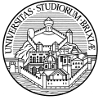
\includegraphics{Logo} 
\end{minipage}\hspace*{\fill} 

 % University/department logo - uncomment to place it

\vfill
\end{center}
\end{titlepage}

%----------------------------------------------------------------------------------------
%	ABSTRACT PAGE
%----------------------------------------------------------------------------------------

\begin{abstract}
\addchaptertocentry{\abstractname} % Add the abstract to the table of contents

%The Thesis Abstract is written here (and usually kept to just this page). The %page is kept centered vertically so can expand into the blank space above the %title too\ldots

\begin{flushleft}

L'esperimento AEgIS al CERN si pone l'obbiettivo di verificare il principio di interazione debole per l'antimateria. Questa tesi presenta un'applicazione web, creata per semplificare il processo di analisi di dati fisici nell'esperimento AEgIS, chiamata "gAn Web". L'analisi può essere svolta da linea di comando in sistemi Unix, ma un'interfaccia grafica può assicurare una migliore user experience, facilitare l'addestramento degli utenti e aumentare la loro produttività. Una web application è un modo intelligente per implementare questa interfaccia perchè permette agli utenti di evitare il processo di installazione e di centralizzare tutte le eventuali modifiche. Questo documento spiega le scelte fatte durante lo sviluppo di questa applicazione e mostra il processo di progettazione che ha portato al risultato finale.



\par\medskip

The AEgIS Experiment at the CERN aims to verify the weak interaction principle for antimatter. This thesis presents a web application designed to simplify the analysis of physical data under the AEgIS experiment called "gAnWeb". This analysis can be run via command lines in a Unix Terminal, but a graphical interface can ensure a better user experience, ease the user training and improve the productivity. A web application is a smart way to implement the interface because it allows users to avoid installations, and centralizes all the eventual modifications. This document explains the choices made during the development of this application and shows the design process that led to the final product.


\end{flushleft}


 
\end{abstract}


%----------------------------------------------------------------------------------------
%	LIST OF CONTENTS/FIGURES/TABLES PAGES
%----------------------------------------------------------------------------------------

\tableofcontents % Prints the main table of contents

\listoffigures % Prints the list of figures

%\listoftables % Prints the list of tables


%----------------------------------------------------------------------------------------
%	THESIS CONTENT - CHAPTERS
%----------------------------------------------------------------------------------------

\mainmatter % Begin numeric (1,2,3...) page numbering

\pagestyle{thesis} % Return the page headers back to the "thesis" style

% Include the chapters of the thesis as separate files from the Chapters folder
% Uncomment the lines as you write the chapters

% Chapter 1

\chapter{Introduction} % Main chapter title

\label{Chapter1} % For referencing the chapter elsewhere, use \ref{Chapter1} 

%----------------------------------------------------------------------------------------

First of all it is important to understand at least generically what is the AEgIS experiment at the CERN and which are its goals. The acronym AEgIS stands for "Antimatter Experiment: gravity, Interferometry, Spectroscopy", this research aims to verify the weak equivalence principle for antimatter. In the first part of this chapter some particulars are explained about this experiment, in the second part is introduced gAn Web, the main topic of this document, the application that allows the physicists to do data analysis in the AEgIS experiment environment easily, through a web interface. 

\section{The AEgIS experiment}


\begin{figure}[H]
\centering

\includegraphics[scale=0.25]{aegisLogo.png} 
\caption{AEgIS's Logo}
\end{figure}

The weak equivalence principle, also known as universality of free fall, states that in the same field all bodies fall with the same acceleration, regardless of the mass and the composition. This principle has been thoroughly tested for the matter, but not for the antimatter: the most important goal of AEgIS experiment is to measure the weak equivalence principle for the antimatter; to test the universality of free fall, AEgIS will attempt to measure the gravitational interaction between matter (the Earth) and antimatter (antihydrogen). Antihydrogen is the antimatter counterpart of hydrogen, it is the simplest atom built with antimatter (see below for a description of its components). The first antihydrogen in an electromagnetic trap has been produced by the ATHENA experiment in 2012 (\url{http://www.nature.com/nature/journal/v419/n6906/full/419439a.html})
with the contribution of a group of the University of Brescia.

The AEgIS experiment is the result of a wide and international scientific collaboration, as visible in the figure 1.2.

\begin{figure}[H]
\centering 

\includegraphics[scale=0.5]{aegis_collaboration_institutes.pdf} 
\caption{Aegis Collaboration institutes}
\end{figure}


In the context of neutral antimatter, the gravitational interaction is of high interest, because it can potentially reveal new forces that violate the weak equivalence principle. Thomas Phillips, from Duke University, says: "If antimatter fell down faster, it would mean the discovery of at least one new force, probably two. If it fell up, it would mean our understanding of general relativity is incorrect". In a practical point of view AEgIS tries to measure the time of flight and the vertical displacement of antihydrogen, with a moirè deflectometer: this process is quite complex, and it is easier to explain it using the following figures (1.3, 1.4 and 1.5).

\begin{figure}[H]
\centering 
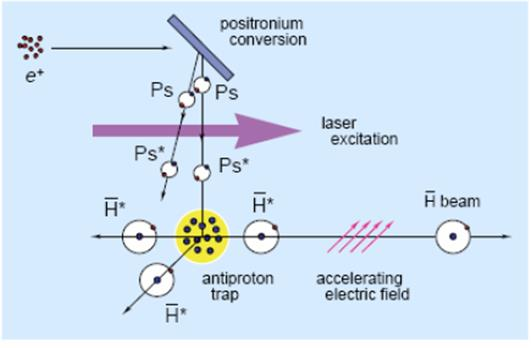
\includegraphics[scale=0.5]{AEgISScheme.png} 
\caption{AEgIS's Scheme, taken from "AEgIS experiment at CERN: measuring antihydrogen free-fall in Earth’s gravitational field to test WEP with antimatter"}
\end{figure}

In the 1.3 figure we can see the process that allows to create through a so called "charge-exchange" reaction antihydrogen. In few words, to create antihydrogen two ingredients are needed: antiprotons and positrons. The antiprotons are provided by CERN, while positrons are produced by the experiment with a radioactive source. To correctly explain this process it is better to start with some definitions:


\begin{enumerate}

% 1
\item Positron: it is the correspondent of the electron in the antimatter. It is an antielectron, that is an electron with positive electrical charge. It is indicated by "e$^{+}$".

% 2
\item Positronium: it is an unstable system consisting of an electron and a positron, bound together into an exotic atom. It is indicated with $ {Ps} $.

% 3
\item Antiproton: it is the antiparticle of the proton. Antiprotons are stable, but they are typically short-lived since any collision with a proton will cause both particles to be annihilated in a neutron and to disappear creating other particles. It is indicated with $ \overline{p} $ (pronounced pbar).

% 4
\item Antihydrogen: it is the antimatter counterpart of hydrogen. Whereas the common hydrogen atom is composed of an electron and a proton, the antihydrogen atom is made up of a positron and an antiproton. It is indicated with $ \overline{H} $ (pronounced hbar).


% 5
\item Antiproton trap: a device that uses an axial magnetic field to radially confine charged particles, in this case antiprotons.


\end{enumerate}

\begin{figure}[H]
\centering
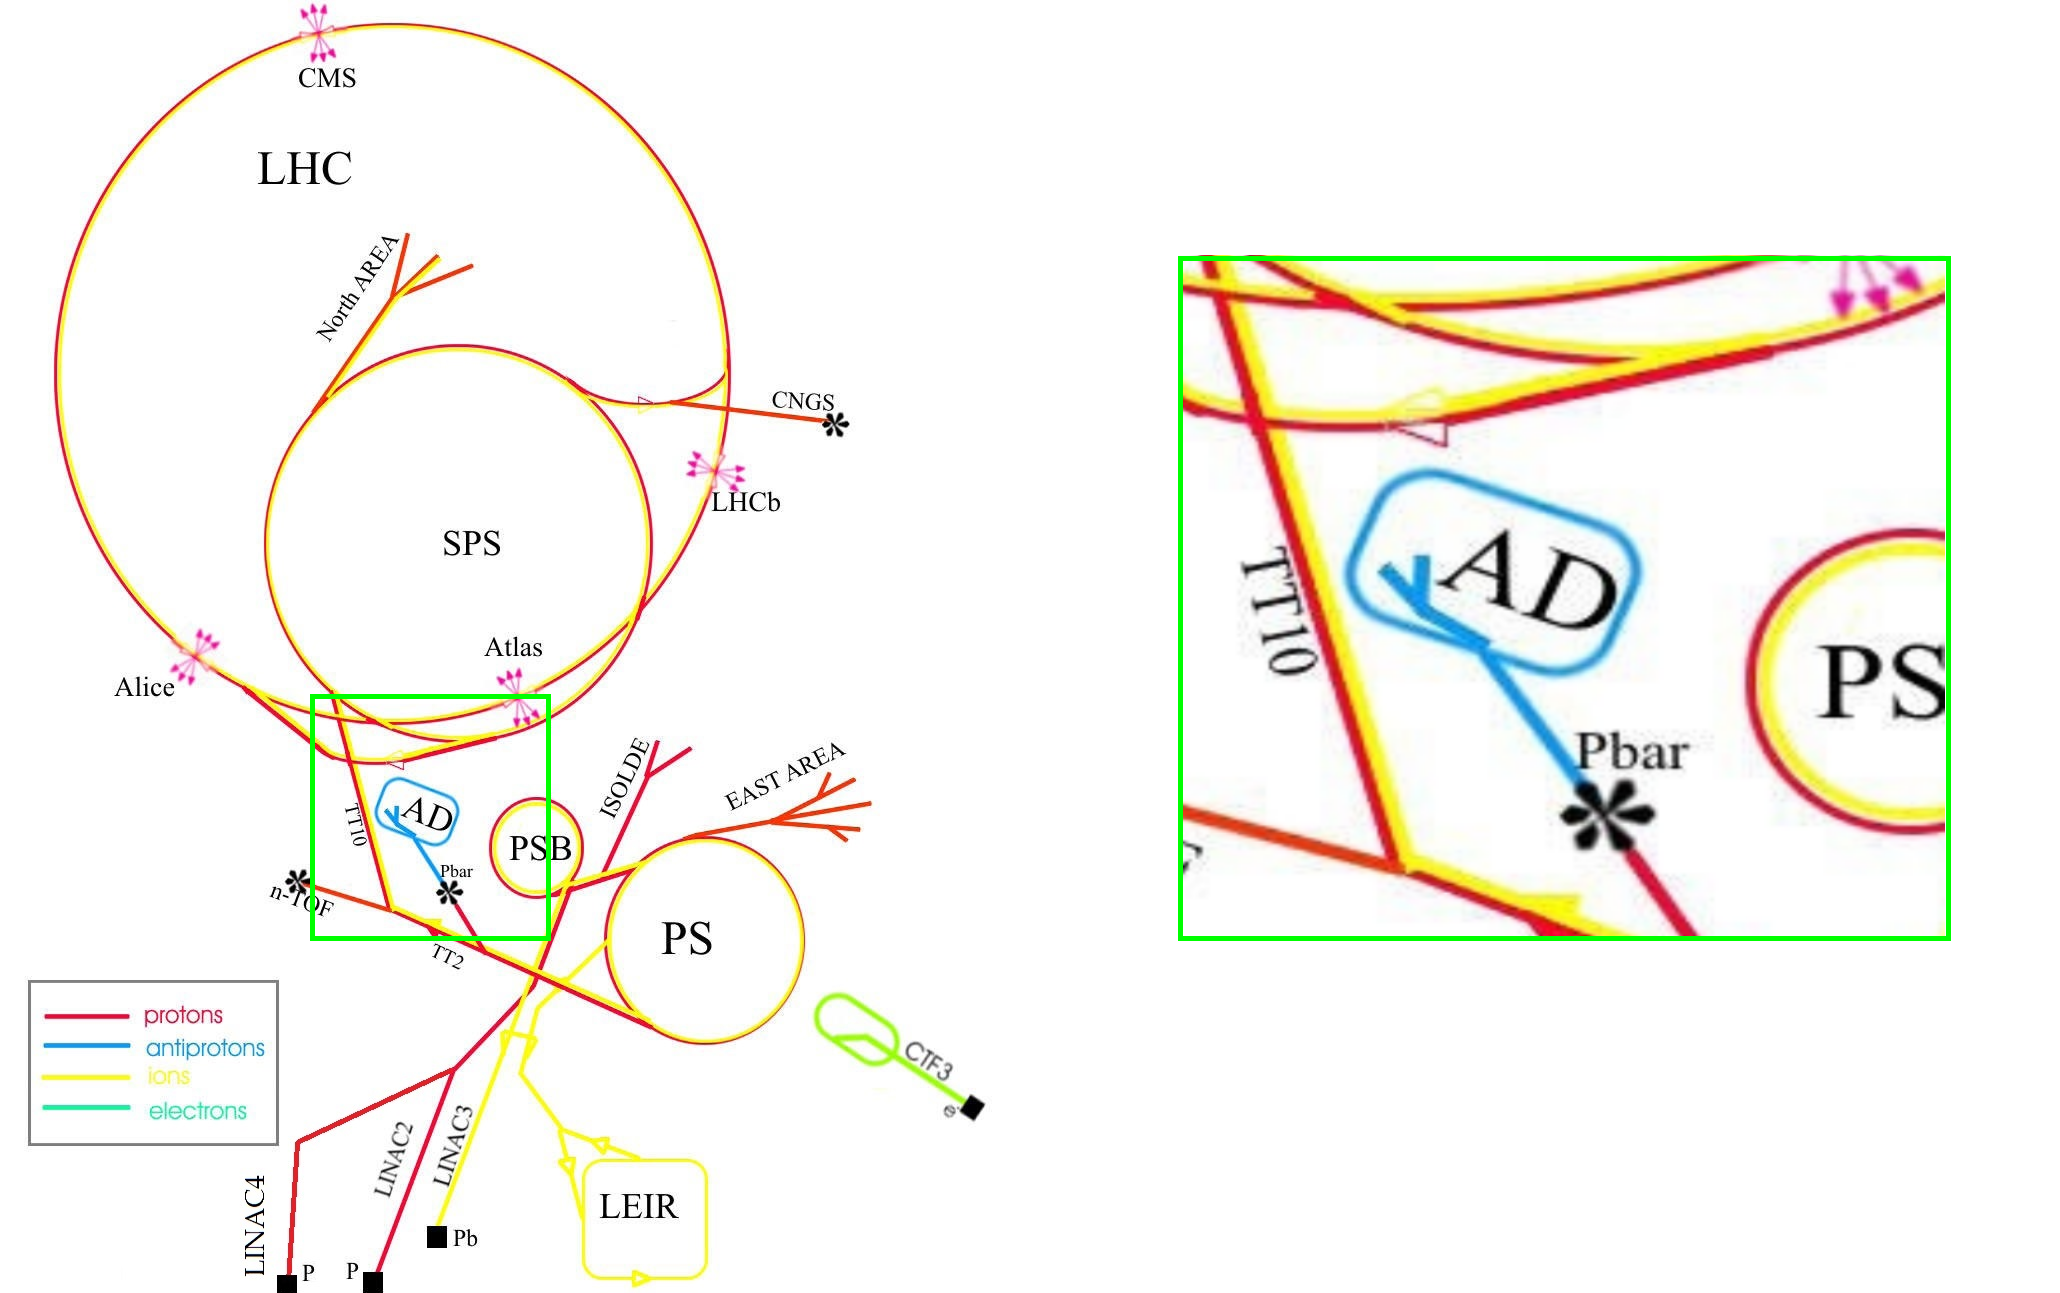
\includegraphics[scale=0.25]{CERNaccelerators.png} 
\caption{ As shown in this figure, AD in a ring in the CERN accelerator system, the AEgIS experiment is part of AD. }
\end{figure}


Antiprotons are provided by the CERN accelerator system and an electric field confines them axially. 
Protons collide with nuclei inside a metal cylinder called "target". About four proton-antiproton pairs are produced in every million collisions, and is possible to separate antiprotons using magnetic fields. The following step is to guide antiprotons toward the AD (Antiproton Decelerator, the ring shown in figure 1.4) where they are slowed down. 
The AEgIS experiment is part of AD, that is a system able to provide a stable source of antiprotons.
To execute AEgIS experiment, antiprotons must be trapped and held inside an antiproton trap, where magnetic fields force the charged antiparticles to spiral around the magnetic field lines, and electric fields confine them along the magnetic axis.

For what concerns positrons, as represented in Fig. 1.3 a beam of positrons (that comes from a $^{22}$Na radioactive source) is accelerated and driven to collide against a "positron-positronium converter" (that is a mesoporous silica film). This process creates positronium, that needs to be excited by lasers, to reach an excited state called Rydberg State. The positronium in Rydberg state is indicated by $ {Ps*} $, it has a longer life than the unexcited positronium, and can be driven to fly into an antiproton trap.


When $ {Ps*} $ is excited by lasers it can combine itself with $ \overline{p} $ to generate excited antihydrogen ($ \overline{H}* $) and electrons. The antihydrogen beam is accelerated using an electric field towards a moiré deflectometer. Then, during the travel it decays to ground state.  


\begin{figure}[H]
\centering
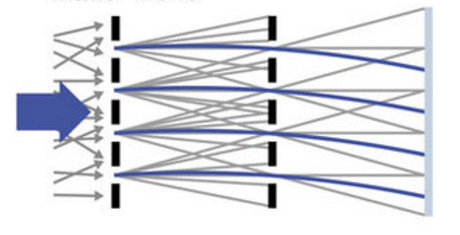
\includegraphics[scale=0.5]{MoireDeflectometer.png} 
\caption{Moiré Deflectometer's Scheme, taken from "http://www.nature.com/articles/ncomms5538" }
\end{figure}

In the Fig. 1.5 a schematic view of a moirè deflectometer is presented.
An antihydrogen beam is thrown toward two subsequent gratings that restrict the transmitted particles to well-defined trajectories. The trajectories are inflected by a force (in this case the force related to $ {m*g} $) and follow a parabolic path. At the final part of the deflectometer there is a detector that shows where the antimatter annihilates, that it is possible to compare the expected trajectories without forces with the obtained trajectories, and measure the force. The proof of principle that such system can be used with antimatter has been realized and operated with $ \overline{p} $s. It showed that a displacement of few $ \mu m $ can be detected with this technique, this result has been published in a Nature [https://www.nature.com/articles/ncomms5538]


\begin{figure}[H]
\centering
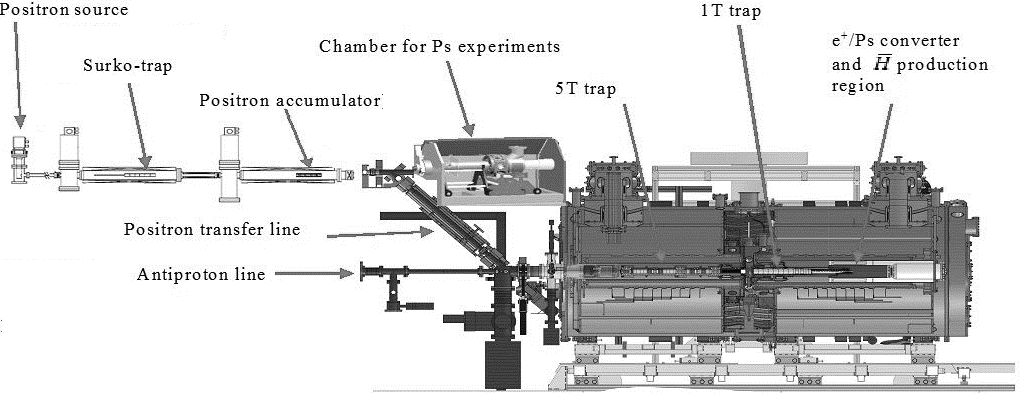
\includegraphics[scale=0.35]{SchemeMachineSetUp.png} 
\caption{AEgIS apparatus set up, taken from "AEgIS experiment at CERN: measuring antihydrogen free-fall in Earth’s gravitational field to test W.E.P. with antimatter" }
\end{figure}

% Chapter 2

\chapter{gAn, gAn Web, and their goal} % Main chapter title

\label{Chapter2} % For referencing the chapter elsewhere, use \ref{Chapter2} 

%----------------------------------------------------------------------------------------

GAn Web, is a web application, equipped with a user friendly interface, based on the most important human-machine interaction principles, designed to allow users to interact with a pre-existing data analysis application named gAn. This chapter aims to introduce information, goals, common aspects, and limits of these applications.

\section{What is data analysis?}

The main goal of gAn Web is to analyse rapidly data extracting important information, so can be useful give some preliminary information about the concept of data analysis.

According to the John Tukey's definition data analysis is: 

"Procedures for analyzing data, techniques for interpreting the results of such procedures, ways of planning the gathering of data to make its analysis easier, more precise or more accurate, and all the machinery and results of (mathematical) statistics which apply to analyzing data" 
( \url{http://projecteuclid.org/euclid.aoms/1177704711} [3]).

The basic idea is that in the modern world almost each activity can provide a big amount of data, but only a few of them are really useful to gain interesting information. The data analysis is a structured process that allows to select the most important parts of this row data and exploit them to gain information able to answer questions, test hypotheses and approve or disprove theories.
In the following figure (2.1) we can see the schema of this process. 

\begin{figure}[H]
\centering
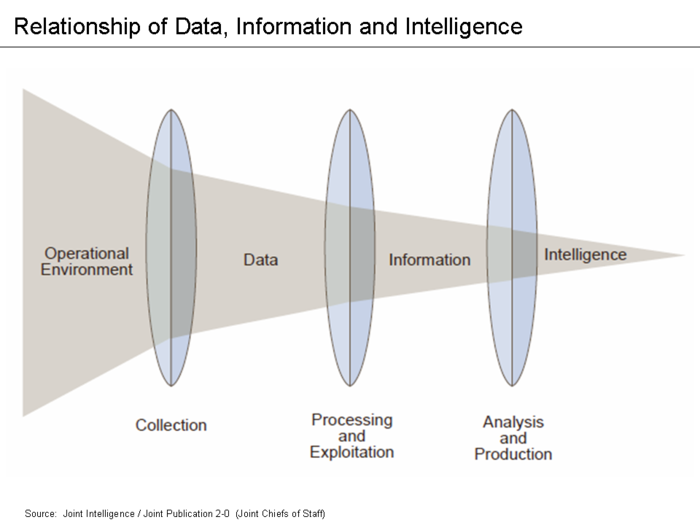
\includegraphics[scale=0.5]{DataAnalysisProcess.png} 
\caption{Here is visible a basic schema of data processes and analysis}
\end{figure}

Data analysis can be divided in some steps:

\begin{enumerate}

% 1
\item Data collection: data can be collected in a variety of ways. For example is possible to collect them using sensors in the environment, such as satellites, recording devices, physical sensors and so on. It is also possible to obtain data through interviews, downloads from online sources, or reading documentation... so the analysis is feasible with a large variety of kinds and sources of data. 

% 2
\item Data processing: raw data must be well-organized for analysis: for example, placing data into row, columns, vector, and so on (but the definition of "well-organized" in this context varies according to the kind of analysis to be performed).

% 3
\item Data cleaning: Once pre-processed and organized, the data may be incomplete, contain duplicates, or contain errors. Data cleaning is the process of correcting these errors, eliminating duplicates and handling incomplete data. Some ways to do this are record matching (comparison between the records to find if there is something suspicious), validation of data (if there is the certainty that data values has to respect some limits), overall evaluation of quality of existing data, de-duplication (process used to remove duplicates). For particular kinds of input this process is very complex (for example vocal input needs an advanced spell-checker), for others is simple (for instance online-survey interviews made using closed choices) 

% 4
\item Exploratory data analysis: in this step the data is analyzed. There are a variety of techniques referred to as "exploratory data analysis", they aim to begin understanding the real content of the data. This process may result in Descriptive statistics, such as the calculation of average or median, or in Data visualization, that allows to examine the data in graphical format, through graphics and other graphical objects.

% 5
\item Modeling and algorithms: another step is using mathematical models to find relations between different variables, such as causality or correlation. An example of this process is the regression analysis.

% 6
\item Communication: this is the final step. It is important to find a way to report the obtained information to the user in an understandable format. The communication must be adapted to the different users, in order to let the data analysis able to meet their requirements.

\end{enumerate}
According to an article written by Andrew Birmingham and Anna Russell (\url{https://which-50.com/this-is-what-big-data-}	\\ \url{really-looks-like-cern-the-universe} 	\url{-and-everything} [4]) in the particular domain of the particles physics this kind of analysis is very important: some experiments at the CERN represents about 150 million sensors delivering data 40 million times per second. There are nearly 600 million collisions per second. This is not the exactly kind of AEgIS experiment, that doesn't generate this gigantic amount of data, but, the point is that not all this information is scientifically interesting. In the huge amount of collisions discussed previously there are only around 100 collisions of interest per second.
This leads a big problem: it is difficult to find a rational way to work with flows of data having this size, and it is strongly required to take only the part of the data actually relevant for the scientific analysis, but it is also important to avoid wasting anything interesting in this dataset.

Another problem to solve to meet the user's requirements is related to the speed with which physicists develop and change focus in their experimental work: they are not interested always at the same things, and they cannot predict in advance what they will need in a remote future, because their needs are related to the process of experimentation, and can change continuously. 
Therefore a system of analysis must be very flexible and dynamic, always ready to serve to new requirements, always able to find exactly what is the "interesting" part of data.  

This kind of problems are not just CERN's problems, they are common in major research centers. Bob Jones, Project Leader at CERN, says:
"CERN is a leader but not alone in having to deal with such high data throughput. We expect to see similar scales in other sciences (such as next generation genome sequencing as well as the Square Kilometer Array which will primarily be deployed in Australia and South Africa) and various business sectors linked to the growing Internet of Things in the near future."
(quote taken from \url{http://www.cloudwatchhub.eu/what-big-data-really}	\\ \url{-looks-cern-universe-and-everything} [4])
 
Big data analysis can provide an answer to this problems: with an intelligent and parametrizable process of filtering it is possible to extract only the subset of scientifically interesting information, and delivering them to the users in an organized and structured way, by tables, statistical values, graphical images. 
In this way is possible to improve the productivity of the physicists, exempting them from unnecessary commitments and dynamically meeting their needs. 


\section{User friendly Data analysis: gAn Web}

GAn is a program that is being used to analyze data related to the AEgIS experiment at CERN, while gAn Web is the web interface to gAn, and it is the main topic of this document.

The goal of gAn Web is to allow users to perform analysis through a more friendly web interface, without install nothing on their machine. In the following image there is a schema that shows how the whole system is organized.

\begin{figure}[H]
\centering
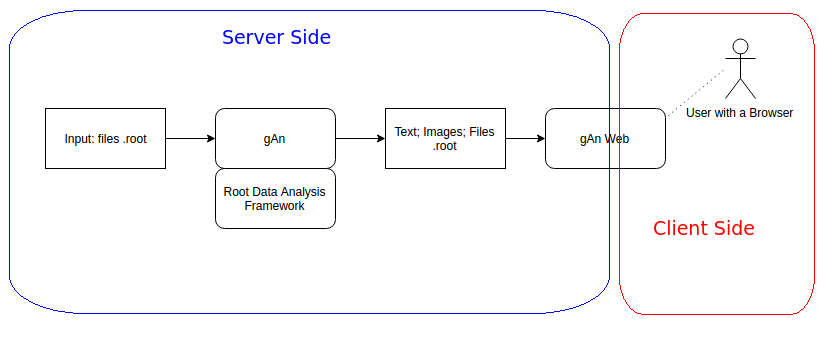
\includegraphics[scale=0.5]{GeneralGAnSchema.png} 
\caption{gAn - gAn Web simple scheme}
\end{figure}

The whole application allows to perform data collection, a process of selection and analysis of data, and data representation. In brief it means being able to extract from a big amount of raw material only the interesting information.

The raw material on which this system works is represented by a set of "Root files". 
The hardware of AEgIS experiment (mostly the detectors) generates these Root files, that are raw, binary files. 
 
The following figure (2.3) presents a schema related to the generation of these input files:

\begin{figure}[H]
\centering
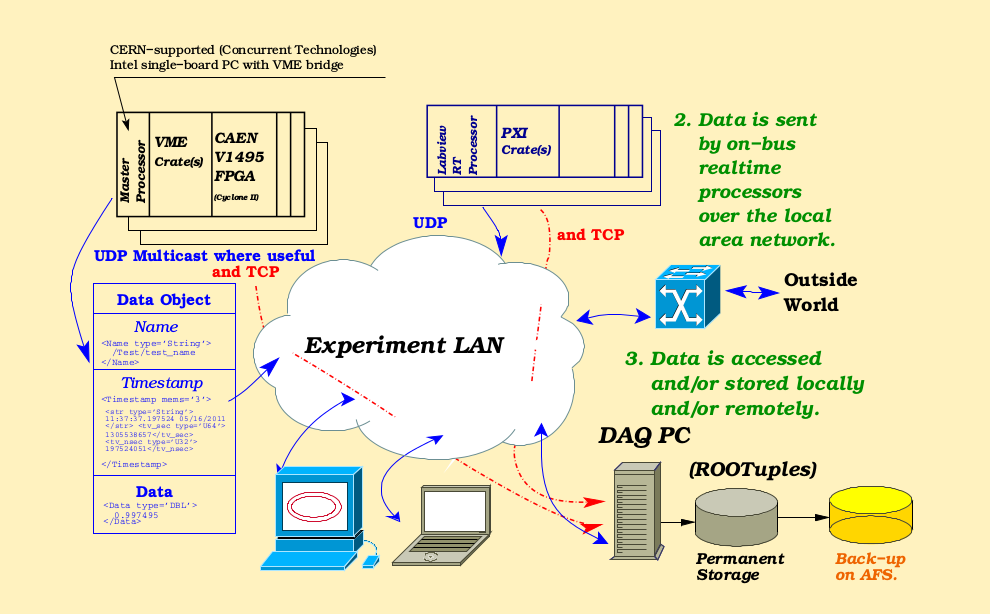
\includegraphics[scale=0.35]{DAQSchema.png} 
\caption{Root format input files generation, DAQ System}
\end{figure}

The data comes from different detectors, that communicate with different protocols, but all the communications use XML as common language. All data are sent through a LAN to a server named DAQ. Here they are stored in the root file to be ready to be analyzed.
The role of DAQ is to cover the first three steps of the data analysis process: it collects, processes and cleans data;

The Root files can be analysed using a framework named ROOT Framework, that consists in a lot of libraries specialized in high-energy physics analysis, and an interpreter able to understand a C++ script.
GAn use this framework, it can access these Root files, make an ordered and organized analysis, extract the most important information, and produce an output that consists of a text with the most important information, comments, and eventual error logs, graphic material such as images of various kind, some other Root format files, with some features used by gAn Web to make further graphical processing, related to the generation of dynamic graphics and figures. 
The goal of gAn is to reduce the big amount of raw data received in input in a little amount of scientifically interesting and easily understandable data in output, covering the forth and the fifth step of the data analysis process: exploratory analysis and modelling and algorithms.

gAn is an application developed in C++ using Object Oriented programming, making 
use of the ROOT (see Section. 2.3 for details) framework. It can be executed in a computer where ROOT 
is installed, inside the root environment with the following line command: 
\begin{verbatim}
prompt>root
root[].x rungAn.C(run_number, "analysis_file")
\end{verbatim}

where "run\_number" is a number identifying the data to be analysed (see below for a description of 
a "run") and "analysis\_file" is a string corresponding to a specific analysis on the data (each analysis
correspond to a unique analysis class, with its .C and .h files.


In order to give the correct information gAn require some inputs from the users.

The input parameters inserted by the users are:
\begin{enumerate}

% 1
\item "Run Number", that identifies in which part of the data the user is interested. 
The time in this experiment is divided in "runs" (a run lasts about some hundred seconds), so the user, by the run parameter can tell to gAn in which time slice he is interested. For example: run 55614 means that the user is interested in the information related to the 22th of November 2016, taken in the time slice between 15:45 and 15:47. 
The enumeration of the runs is incremental: so the run 55199 identifies the time slice immediately after the time slices identified by 55198. The progress of the run numbers is always going on, so new run numbers are continuously added. 
In this document every time we say "last run number" we don't mean the absolute last run numbers, but the run number that is going on right in this moment. This concept is important because usually the users use gAn Web on the last existing run number (so on the run number that is going on right at that moment) or on the immediately previous run number.  
This system used to identify time slices seems to be strange at the beginning but is a standard for all the applications in the AEgIS experiment and it allows a very efficient and precise communication. It is indeed a standard in all the experimental activities in high-energy, nuclear and particles physics. This is because inside a "run" there are data related to a specific experimental "configuration".

How can the user have more information about the runs? 
There is a RunLog (sometimes also called LogBook). The RunLog is a document organized by date on which for each run essential and specific information are reported, such as the run number, the date of acquisition, the experimental configuration, and other notes that the physicist that performed the data taking consider important to record.

% 2
\item "Type of analysis", that identifies what gAn must do with the data and what it must show as output to the user.
An analysis is basically a series of operations that treat the data to produce specific output. For example the user can look at the images regarding positrons and antiprotons and calculate the number of particles. Another example is that the user can calculate the fraction of particles that reached the end of the experiment, and so on. Each "analysis" corresponds to a specific source file that gAn loads and run accordingly.

\end{enumerate}


The output of gAn consists of a single text file with computed, (quite) organized data, and a folder of images in png format.
This structure (root files in input, data analysis using Root, images, organized and selected data in output) is very common in the CERN's experiments. 
The output of gAn is quite understandable by an experienced physicist, but it is disorganized, complex for an untrained user, and the terminal interface can be surely improved using some more user friendly technologies.

GAn Web is a web application, that aims to create a user friendly web interface, based on the most important human-machine interaction principles, between the users and gAn. 

A web interface can improve the system in two ways:

\begin{enumerate}

% 1
\item gAn is a stand-alone program based on ROOT, that can be installed on the user's machine; the user has to install the correct version of ROOT to avoid compatibility problems (ROOT is still not perfectly version independent: different versions can occasionally lead to different behaviors). Furthermore, this kind of program is continuously changing, the performed analysis is continuously improved (in the first 2 weeks from the debut of the program there were already several kinds of analysis, because often at the changing of the needs the programmers creates new analysis), so the installed version of gAn is not unchangeable, and the user must often update it. Instead, a centralized version installed on a server, with services accessible from a normal browser by the user can avoid (or at least reduce) this kind of problems and be more usable.    
 

% 2
\item a Linux terminal interface is practical for expert users, but a web based interface can be more attractive for new users, and, if well done, can be easier to use. It is important to notice that all the terminal-based applications exploit the users memory and are prone to errors.


\end{enumerate}



\section{ROOT - Physical Data Analysis }

There are some software (often free software) specialized in the analysis of data. Each of these software has strengths and weaknesses, and none of them appear to be absolutely better than the others. Following there are some examples:
 
\begin{enumerate}

% 1
\item MATLAB (matrix laboratory) is a numerical computing environment. It is a proprietary (t is not available for free, and it is quite expensive) programming language developed by MathWorks. Matlab allows matrix manipulations, plotting of functions and data, implementation of algorithms, creation of user interfaces, and embedding programs written in other languages, including C, C++, Java, Fortran and Python. 
Some detractors say that the statistical support is incomplete if compared with other solutions (also free).

% 2
\item R is a programming language and a software environment for statistical computing. It is supported by the R Foundation for Statistical Computing.The R language is widely diffused for developing statistical software and for data analysis. His popularity has increased in recent years, this is due to the fact that R is free and provides to user a good front-end interface. On the other hand some users say that the learning curve is quite hard at the beginning (in a big research center this is not a big problem..).  

% 3 
\item SciPy/NumPy/Matplotlib are libraries that work in the field of data analysis written for the general purpose language Python. It is a quite immature technology, but it is freely available and it uses a general purpose and widely diffused language like Python.

% 4
\item ROOT is an object-oriented program and library developed by CERN, released the first time in 2003 (the process of development started in 1994 and it has been continuously updated until now). It was originally designed for particle physics data analysis and contains several features specific to this field, but it is also used in other applications such as astronomy and data mining. 

\end{enumerate}

For the AEgIS experiment ROOT is the chosen software to carry out the activities of data analysis. The reason is that this software has been specifically tailored to meet the requirements of the analysis applied to particle physics.
Another advantage of ROOT is that there are a lot of libraries created during the years related to the activities of the experiments of the CERN and it is nearly impossible to rebuild them from scratch with another software.

ROOT development was started by René Brun and Fons Rademakers in 1994 (but a more extended and precise list of collaborators is accessible here \url{https://root.cern.ch/root/htmldoc/guides/users -guide/ROOTUsersGuide.html#preface} [5]). 
The ROOT's user guide start with this prefaction, that explains in detail how ROOT was born:
"In late 1994, we decided to learn and investigate Object Oriented programming and C++ to better judge the suitability of these relatively new techniques for scientific programming. We knew that there is no better way to learn a new programming environment than to use it to write a program that can solve a real problem. After a few weeks, we had our first histogramming package in C++. A few weeks later we had a rewrite of the same package using the, at that time, very new template features of C++. Again, a few weeks later we had another rewrite of the package without templates since we could only compile the version with templates on one single platform using a specific compiler. Finally, after about four months we had a histogramming package that was faster and more efficient than the well-known FORTRAN based HBOOK histogramming package. This gave us enough confidence in the new technologies to decide to continue the development. Thus was born ROOT."
(Taken from \url{https://root.cern.ch/root/htmldoc/guides/users-guide/ROOTUsersGuide.html#preface} [5])


This software is partially released under GPL (this means that everyone is allowed to use, redistribute and change the software, but any changes made must also be licensed under the GPL), and partially under LGPL (The LGPL is similar to the GPL, but is more designed for software libraries in that the developer wants to allow non-GPL applications to link to your library and utilise it).

ROOT is an object oriented framework that aims to solve problems related to high-energy physics. To better understand what is ROOT is important to start with understanding what is a framework: in IT a framework is a structure that helps the programmers providing them a set of already working utilities and services (for example, I/O, graphics, etc.) often related to the sector in which the framework aims to work (for example, the services of a web development framework are related to the layout of a web page, to the organization of DBs etc.). ROOT in particular offers services, functions, and packages related to the world of high-energy physics research, that allow to save much work.
It provides, for example the possibility to use a computer's graphics subsystem and operating system with abstraction, allowing the developer to create a graphical user interface and a GUI builder. ROOT provides also an abstract platform that allows to run C++ and command line scripts. More precisely ROOT includes (among others):

\begin{enumerate}

% 1
\item Libraries related to histogramming and graphing, that allows the developer to easily represent graphically statistical distributions. Also 3D visualization is allowed.

% 2
\item Libraries related to regression analysis.

% 3
\item Various statistics tools. 

% 4
\item Libraries related to digital image processing and manipulation.

% 5
\item Libraries aimed to allow parallel computing, (to parallelize data analysis can be really useful in order to manage the complexity of the calculations).

%6
\item The possibility of interfacing in both directions with code written in Python or Ruby.

%7 
\item The possibility of interfacing with Javascript, allowing the developer to access ROOT functionalities by a Browser.

\end{enumerate}

In the following figure (2.2) we can see the structure of the ROOT's libraries:

\begin{figure}[H]
\centering
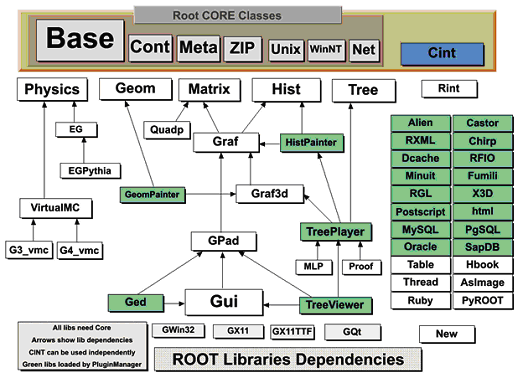
\includegraphics[scale=0.5]{RootStructure.png} 
\caption{ROOT structure}
\end{figure}


 
% Chapter 3


\chapter{User Interface } % Main chapter title

label{Chapter3} % For referencing the chapter elsewhere, use \ref{Chapter1} 

%----------------------------------------------------------------------------------------

% Define some commands to keep the formatting separated from the content 
%\newcommand{\keyword}[1]{\textbf{#2}}
%\newcommand{\tabhead}[1]{\textbf{#2}}
%\newcommand{\code}[1]{\texttt{#2}}
%\newcommand{\file}[1]{\texttt{\bfseries#2}}
%\newcommand{\option}[1]{\texttt{\itshape#2}}


\section{Human Machine Interaction principles}
todo todo

\section{Web interface vs Java Fx vs Xojo}
todo todo

\section{Used Technologies and Framworks}
todo general

\subsection{PHP}
todo particular

\subsection{Javascript}
todo particular

\subsection{Bootstrap}
todo particular

\subsection{Sass}
todo particular

% Chapter 3

\chapter{First version} % Main chapter title

\label{Chapter3} % For referencing the chapter elsewhere, use \ref{Chapter1} 


This chapter analyses which are the requirements of gAn Web at the first version and how they are implemented. This first version is very incomplete and aesthetically very raw, but very useful because it is meant to be a "test" to understand how to implement some functionalities and a base from which start to discuss with the super-users. 

\section{Functional requirements}
The definition of functional requirements aims to specifying in detail what the web application can do, and in which way an user can use it. The development of gAn Web is divided in three stages, so the requirements are peculiar and different for each stage. The first version (from now "gAn Web v1") is a very simple application: instead of access the program by a linux terminal like gAn, in gAn Web v1, the user can use the program through a graphical interface. 
The requirements of this version are the following:

\begin{enumerate}

% 1
\item The user, in the homepage, can choose the run (only one run, for the moment) in which he is interested, using an input field. This field has a validator, able to understand if the run number is inserted, if it is effectively a number, and if it is in an acceptable range. The user receives an explaining and precise error message directly on the homepage if the input field is empty or if the inserted value is not acceptable. Is it always possible validate the inserted run and ensure that the related Root file exists? No, because in some moments some sensors don't work properly and it is inevitable that some root files related to some runs are incomplete, or even in-existent. This problem will be solved in the next versions.

% 2
\item At this moment there is only a generic idea about what kind of analysis can be useful for the user, so in this version there will be only a generic analysis, able to dump in text all the possible information, and a group of example images (this is useless for the goal of the scientific research, but very useful to improve the understanding of the needed features of the web interface).
At this stage is not clear if the type of analysis will be chosen by the user of automatically selected by the program , so in gAn web v1 there are no buttons able to allow the user to select the type of analysis (this point will be reconsidered in next versions).

% 3
\item The user can start the program with a single click, by a button (usable only if the inserted number is valid).

% 4
\item When the program is executed the user can see the text output on the screen. This text is clear for a physicist (it is not clear for a person who doesn't have a specific preparation). This is an important point: there are big differences between the domain of the software engineering and the physics, so is better that this textual output is written by the hand of a physicist, to ensure to avoid misunderstanding due to different meanings assigned to symbols in different domains. Improve the legibility of the output will be a requirement for a more advanced version. 

% 5
\item When the program is executed the user can see the output images by clicking a button that link to an images-page. The images are ordered and organized by groups (the groups are related about which sensor takes the information necessary to create the image). The user can decide if he prefers to see the image in a little, medium or big format. The user can also decide if the images are distributed in the screen vertically or through a "carousel layout". The user can access the image in full-screen by clicking on it: he is redirected to a page with the image shown in full screen, and can return to the all-images page by a return button. It is absolutely important to understand exactly which information are interesting for the users, and show in the images only them and all of them, this point will be solved with a confrontation with the pilot-users. 

%6
\item The user can modify a configuration file (a .txt file on the server), by a web interface. In this file there are some values the need to be set (otherwise it uses default values), and the user can do it by radio buttons (in this way he is forced to choose valid values). This configuration file can modify the way in which gAn works and modify the resulting output (both the text and the images).   

\end{enumerate}

 
\section{Non-functional requirements}

This version (and actually also all the next versions) has some non-functional requisites:

\begin{enumerate}

\item The first is quite simple: gAn Web has to ensure that in case of crash of the program the web server mustn't crash too. The point is that on this web server (Apache server, installed on Linux) there are some other important applications, so, if gAn web crashes it is not a big problem, but the crash cannot force Apache, or worst the entire machine, to stop or restart. 
This requisite is quite easy to meet: a modern web application based on Html, Javascript, PHP and CSS is quite safe, a general crash of the server it is very unlikely to happen. If the C++ application or some Root libraries crashes (for example if the user asks for an inexistent run) the web application gracefully warn the user about the problem, but without uncontrolled behaviors.  

\item The application must work without install nothing. Also this requirement is very easy to meet: gAn Web is a web interface, it requires only a browser, nothing else.

\item The application must be compatible with any machine (except mobile phones, not requested), regardless of hardware, operating system, installed software. Also this requirement is achieved because of gAn Web only needs a browser to be used. A good observation is that the application is typically used on the computers of the AEgIS control room, that have a quite big screens, but to be sure is better to create an application able to adapt itself also to (quite) little screens.  

\item The application must be easy to be modified and extended in the future by persons who aren't necessarily software engineers. The point is that the student who wrote this program is a "momentary collaborator" in the AEgIS experiment, and all the modifications to the program must be done by other people, in most cases physicists. So the best way is to comment in detail the code and keep the code simple (this is a basic good-programming requirement).   


\end{enumerate}

\section{Scenario based functional analysis}

Following there are a list of scenarios in which a user achieves a goal by doing a list of steps. The goal of these scenarios is to show in detail how the interaction between the user and the system takes place. In this first version, the complexity of the scenarios is very low. 

\begin{enumerate}

\item The user in interested in the run 31111. In particular he is interested in the peak (the highest value) reached by a sensor named Mimito (this kind of task is very common). At this stage we still not work with kinds of analysis. The user, opened a browser in the homepage, inserts the run number and push "Send". He waits some seconds (there is a progress bar) and he arrives in a textual output page. At this point he can search in the text the information in which he is interested (it is a numerical value). Probably he is interested also in a image, to understand spatially where this peak is: he clicks on the "Show Images" button, he goes in the images pages, he selects the group "mimito", and the browser shows him a png image showing an histogram in 3 dimension: on the z-axis there is the peak, he can understand in which place (identified by x-axis and y-axis coordinates), the peak takes place, and how is shaped the resulting 3-d figure. From there he can return to the homepage and do another task.   

\item The user is no more interested in Mimito, but in another sensor: Faraday Cup. The user wants to know what are the values detected by the sensor in the same run (also this scenario is very common, often when the result of a sensor is unexpected, checking the others is interesting). This other sensor is not automatically enabled, so the user goes through the "Edit Configuration" button in a page able to modify the configuration file. Here the user can see a list of sensors, and he can use radio-buttons to modify their values from no (==disabled), to yes (==enabled). The user enables all the sensors, confirms the changes, and automatically returns in the homepage. Now he can like before insert the number, and get the outputs in textual and in images format.  



\end{enumerate}


\section{Prototyping}

This version is very simple and it contains only the basic functionalities. 
The goal of this version are: to understand if this kind of system can be useful for the users, and to experiment some technical solutions to create the features needed to achieve the goals. 

To create a prototype in this case the web programming is preferred on programs able to produce mock-ups, because the designer is quite expert in web development and can produce it quite rapidly, but he is not used to produce mock-ups with specialized software so the production of mock-ups would be slower than the complete development (actually, quite complete). 


Following are visible some part of the first prototype, with very simple features.

\begin{enumerate}
\item The homepage:

\begin{figure}[H]
\centering
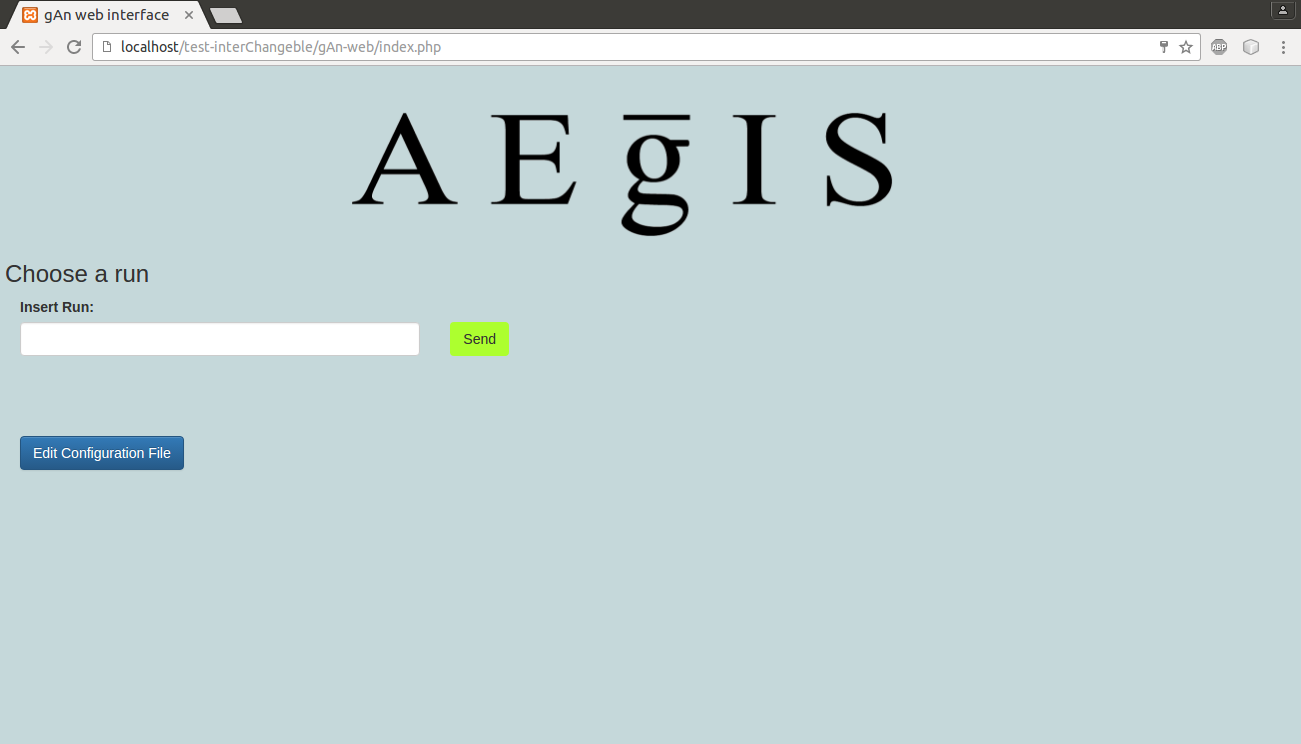
\includegraphics[scale=0.25]{HomePageOLD.png} 
\caption{First version: the first homepage of gAn Web}
\end{figure}

It is quite clear: There is the AEgIS Logo, an input field where the user can insert a run number (only one in this version) and a "Send" button to start the analysis (using gAn). A button "Edit Configuration File" allows the user to  enter in the page dedicated to the configuration of the program.

\item The text output page:

\begin{figure}[H]
\centering
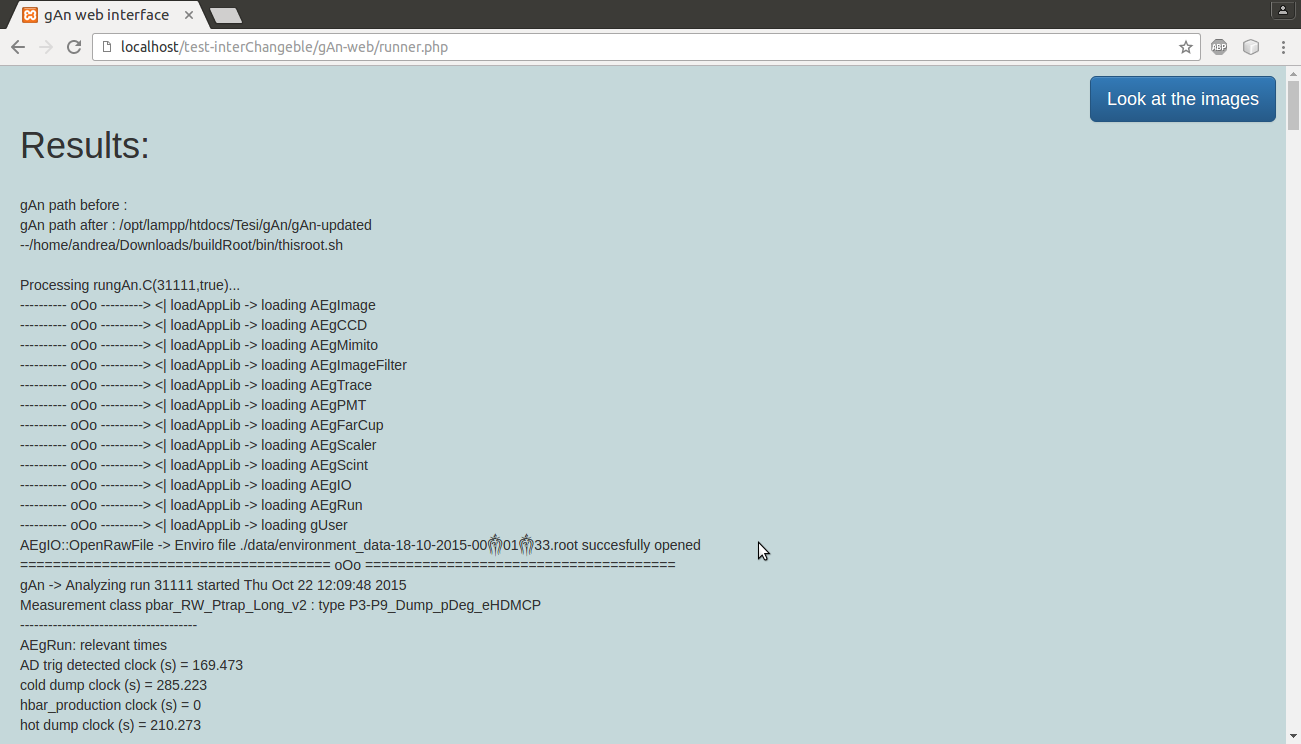
\includegraphics[scale=0.25]{TextOutputOLD.png} 
\caption{First version: the page related to the textual output of gAn Web}
\end{figure}
  
The textual result of the computation is visible: it seems to be too long and incomprehensible, but for physicists it is quite clear; to understand what is the best way to format this output a further confrontation with the users is needed. The graphics is very minimalist, there is only one button: "Look at the images", that sends the user to the page related to the images. 



\item The page related to the images:

\begin{figure}[H]
\centering
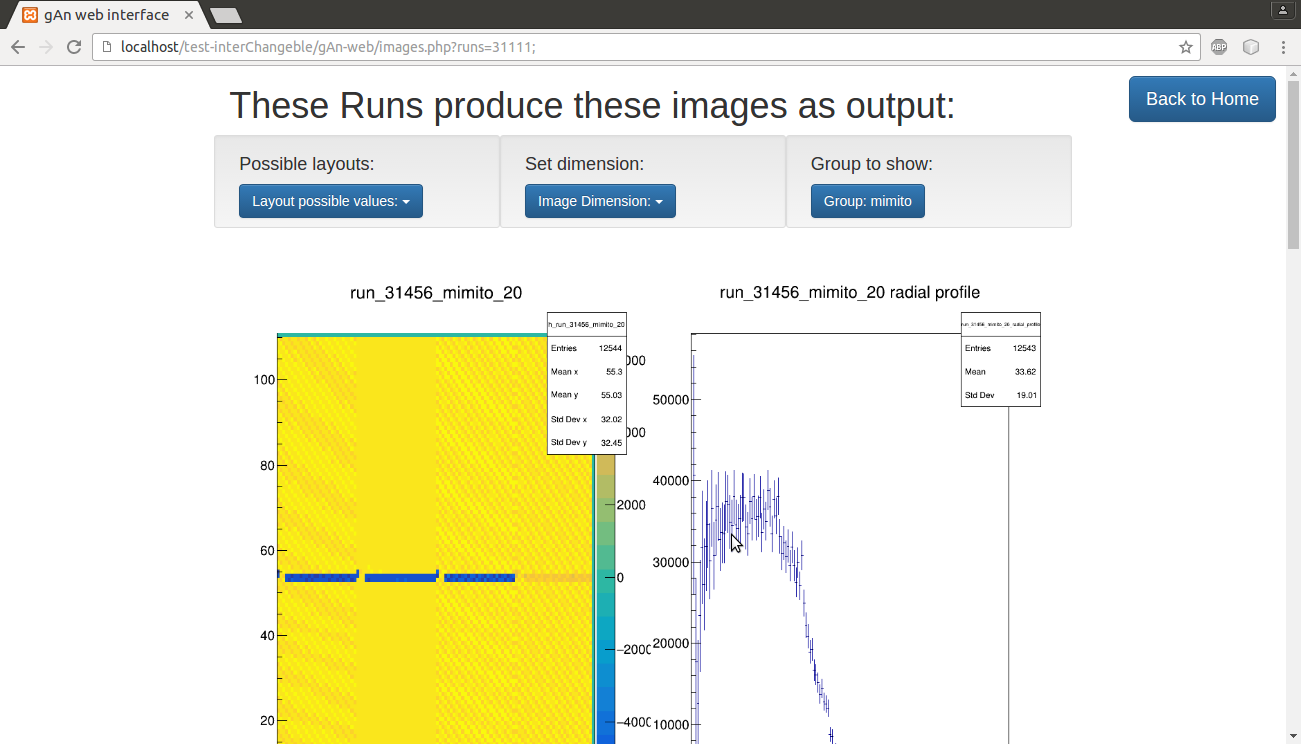
\includegraphics[scale=0.25]{AllImagesPageOLD.png}
\caption{First version: the page able to show the output images in the early prototype}
\end{figure}   

This page shows the images in a dynamic framework, that the user can edit.
The user can choose by dropdown menus the dimension, the layout ("vertical", if he prefers the images disposed vertically one above the other, "carousel" if he prefers the images organized horizontally, navigable by a "next" button and a "previous" button), the group to show (each image belongs to a group, each group usually is composed by 2-3 images). Clicking on a image the user can open it in a full page version (but it is still a static image, a png).


\item The page that aims to edit the configuration file:

\begin{figure}[H]
\centering
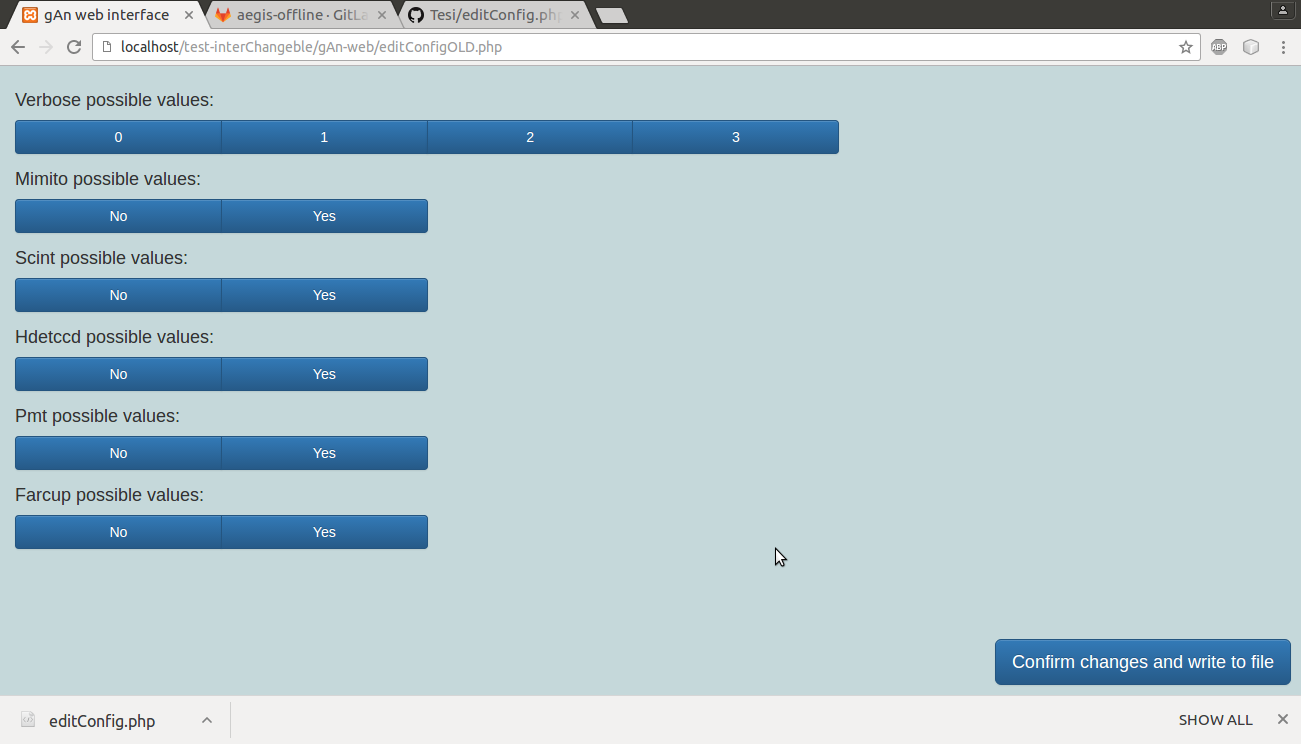
\includegraphics[scale=0.25]{EditConfigOLD.png}  
\caption{First version: the configuration page}
\end{figure}   

This page allows the user to choose by radio buttons (modified using Bootstrap graphic) the value to insert in the configuration file of gAn. Radio buttons force users to insert correct values.    

\end{enumerate}

\section{How the early version can be improved}
The early version's goal is just to be a demo. In particular, it is based on the assumption that the user knows in every moment all about gAn (how does it work,  what is the meaning of each field of the configuration file, and so on). It can be improved literally in every point, according with the principles of the Human Computer Interaction.

 
% Chapter 5

\chapter{Intermediate version} % Main chapter title

\label{Chapter5} % For referencing the chapter elsewhere, use \ref{Chapter1} 

In this chapter the features of the intermediate version are exposed.

\section{Functional requirements}

The intermediate version (from now "gAn Web v2") is more complex than the first one. It was born from the tips and the observation of the pilot users. In this version we start to think more deeply about what functionalities are more important and how we can let them accessible by the users. The aesthetic is still not very considered at this stage (it will become important in the next stage). 
All the new required characteristics are exposed in the following:

\begin{enumerate}

% 1
\item The user can insert multiple runs: separated by a semicolon (but in case of errors the system can automatically correct them replacing symbols like "-" or "," or "." with semicolons and giving a more robust service). These runs can be inserted by an input field of by a range select button: this button opens a "modal" that allows the user to choose the first run and the last, and automatically insert the comprised runs (for example, if the user inserts 30000 and 30010 the system inserts automatically all the run numbers between 30000 and 30010). This modal has a validation system, that ensures the correctness of the inserted values. It is not perfectly clear if this solution fits the needs of the users, but the tests with the whole users group will probably solve this doubt. 

% 2
\item The user can choose which kind of analysis execute. At this point the different analysis are related to the different versions of gAn that at this stage an heterogeneous group of programmers are developing and uploading on Gitlab. It is not clear which ones of these branches will be permanent or not, so the program must be able to use all of them. The type of the analysis depends on the version of gAn downloaded and used for the execution of the program. In gAn Web v2 five complete branches exist, but in the future they may become more. They are externally very similar, the differences are the algorithms in the program, but they give a different output (different output but in the same format: text and images). 
In this version is not clear if all the different versions will be used for the final application, to clarify this point the best solution is to observe directly the user's behavior. 

% 3
\item The configuration file is not only in text format, but also can be in XML format (it depends on the selected version of gAn). The XML ensures a stronger structure, and must be transparent to the user (he doesn't see differences between the configurator that works with a txt file and the one that works with XML). At this stage both text format and XML format are acceptable, to ensure the retro-compatibility of some analysis, but it is possible that in further versions the XML-based design will become dominant. 

%4
\item The user can choose what version of Root he wants to use for the program. Theoretically different versions of Root are perfectly compatible, but in practice each version of gAn is designed to work with a particular version of Root and to avoid problems it seems to be a good idea to allow the user to choose freely among the installed versions on the server.  

%5
\item The user can save images on his hard disk: he can choose from the shown images in the images page an image to download by clicking on a specific download button near the image. Furthermore there is another button "Download All" with whom the user can simple download all the output images.

%6 
\item The user can download a reduced version of the root file with information about the images and the results: gAn produces this kind of files as "half-processed" during the computing, and it is not a problem to save this on the hard disk of the server in a specified folder. For an expert user can be scientifically interesting to have this file (this root file contains more information than the application's output, the most of this information is useless [it is an "half-processed" file] , but sometimes an expert user can find something interesting), so the user must have the opportunity to download this.     

% 7
\item The super-users prefer the dropdown menu than the radio button, so all the radio buttons in the program are replaced by dropdown menus.

% 8
\item The user has to access not only a png image, but also a root-image. This kind of image is interactive: the user can left-click and drag the mouse to select parts of the image and zoom them, and with a right click perform dynamically some kind of image processing (set colors, choose what kind of chart to show, modify the chart legend, translate in a 3D space the image etc). In this way each user can choose freely which information he wants to see in the image (try to oversee all user's needs in this part seems to be too difficult, to overcome this limit giving him the freedom of accessing the image).
All of this must be done by the user through a browser window. This requisite seems to be quite complex, but Root provides libraries (these libraries work well but they are poorly documented) to interact with Javascript.

% 9
\item In the homepage the user can see the run number of the last root file produced by the machine, and its creation date and time (so, he can understand what is the maximum of the range of the acceptable numbers). Also, the run number is an unit of measurement of the time, so through this number the user can have information about the progress of the experiment. This is an important point because actually in most cases users work with the last existing run or the one immediately before, but the way in which this application can help the user in the selection of the run needs to be deeply analyzed with a test with the users. 

% 10
\item There is a login system: the user must insert a password to use the system. The authentication is based on the comparison between the hash function of the inserted password and the hash function of the AEgIS password. If the password is correct the user receives a cookie, before each action in the site the server requests and checks this cookie to be sure about the identity of the user.  

\end{enumerate}

In the intermediate version there was another functional requirement. Ideally the user should have been able to select a gAn version also if not installed in the server machine: in this case the system should have been capable to automatically search on the AEgIS Gitlab repository the correct version (if existing), download it, unpack it in the server, and use it to execute the program. 
After some discussion this requirement has been canceled, because it was considered complex, basically useless, and potentially harmful (on the branches of the repository there are untested and incomplete versions, that can create if executed wrong outputs, so wrong scientific results). Manually installing the stable versions of gAn on the server seems to be a more smart way to work at this stage.


\subsection{Ambiguities (and related solutions)}

At least a point seems to be still ambiguous: 

The textual output of gAn needs to be formatted in some way to be more organized and clear? 
The answer is difficult: for a non-physicists this output seems to be disordered, too long, with too many groups of information, and very difficult to understand, but on this question the pilot users (that are physicists) questioned answered that the output is clear and doesn't need to be modified or improved in any way. The only requests of the users were about the font and the font-size. To check this fact the best solution probably is to observe the behavior of the users at work, and eventually ask them information about that.
Anyway, in the second version, in case of multiple run selection, there is a "navbar" that allows the user to show only a run-result per time.


\section{Scenario-based functional analysis}

In the following there is a list of scenarios able to describe samples of interaction. In this situation the interaction is more complex than before.

\begin{enumerate}

\item The user wants to analyse the runs between 30000 and 30010, plus the run 31456, to make a comparison, he is interested both in the text-output and in the images: 
the user goes to the homepage, he is redirected to the authentication page and he does the login. If the login is successful the user returns automatically in the homepage, and he can insert the runs between 30000 and 30010 manually separating them with a semicolon or better clicking the "add range of runs" button, that opens a modal, in which the user can insert the minimum and the maximum of the range, and confirm (confirmation closes the modal redirecting the user to the homepage). After the user can add manually the run 31456 separating it from the others with a semicolon. If the inserted run numbers doesn't make sense the system shows on the page an error message. If the inserted run numbers are valid, the user can click the "send" button (before the button was red and disabled, now it is green and clickable) and start gAn. A progress bar is shown, a waiting message appears, and the user waits for some seconds (at this stage of development it is very hard to predict how much time gAn requests to execute). After some seconds the user is redirected in a page that shows the textual results: on the top of the page there is a navbar that shows the computed run numbers: the user uses this navbar to choose what part of the results to show in the screen. This bar is draggable, the user can freely move it. From this page the user can, through the button "show all images", access to another page dedicated to the images. In this page he can configure through dropdown menus the dimension, the layout, the group of the images to show (each image belongs to a group, the group depends on the sensor that generates the data from that the image is generated). He can also, by clicking on a single image, access to another page, with a single image (the clicked image) that is completely accessible: the user can rotate the image, move it in a 3D space, zoom in, zoom out, select part, do some basic digital image processing and choose the kind of chart to show.   

\item The user wants to use the version 5.34 of Root (an old but stable version) to execute gAn: 
he completes the login, in the home page there is a button name "Choose Root version", clicking on this button the user is sent to a page where, he is informed about the current version of Root, and through a dropdown menu can choose among some version of Root already installed on the server (all the acceptable Root versions are installed on the server) . If the 5.34 version is one of the installed versions he can select it and confirm, the goal is achieved. If the 5.34 version is not installed, the user cannot use this version.  

\item The user wants to select the "Rug-dev" branch of gAn:
the process is very similar to the process that allows the user to choose a Root version. The user completes the login, in the home page there is a button name "Choose gAn version", clicking on this button the user is sent to a page where, he, through a dropdown menu, he can choose among some branches of gAn available on the machine. "Rug-dev" is one of these, the user can confirm and the task is completed.

\item The user wants to make the computation using only the data taken from the sensor named "Mimito":
The user, after the login, in the homepage can use the button "Edit Config" to the reach a page where, through some dropdown menus, he can change the configuration file of gAn. Each of the dropdown menus is related to a sensor (often they are 5-6, it depends on the branch), and the option of the dropdown are "yes" or "no": if "yes" is selected the sensor's data are used in the computation, if "no" they aren't. One of the dropdown menus is named "Mimito", the user select "yes" for this sensor, "no" for all the others.  

\item The user wants to download all the images related to the runs 40001 and 40002:
After the login, he can insert the runs in the homepage (it is possible both by input field and by range selector. Two ways to do the same thing: although in the next version this point will be rethought), run gAn, wait the end of the execution, click "Show all images", and from here click "download all images". All the images will be downloaded in png format.

\item The user wants to download the semi-processed root file related to the runs 31111 and 31112:
The steps are the same as the steps used to download the images, but instead of the button "Show all images", the user has to use the button "download root files".     

\end{enumerate}  


\section{Prototyping}

The intermediate version is based on the first version, but it is quite different and re-building from zero the application (re-using only some parts) is maybe the smartest solution. Some pages (and functionalities) are added, some existing pages are improved. 
Also in this case the mock-ups are interactive and really working, the developer chooses to program directly with a common web-development process HTML-javascript-PHP based, to optimize the time.

In the following all modifications are explained.

\subsection{Modified pages}
The homepage:

\begin{figure}[H]
\centering
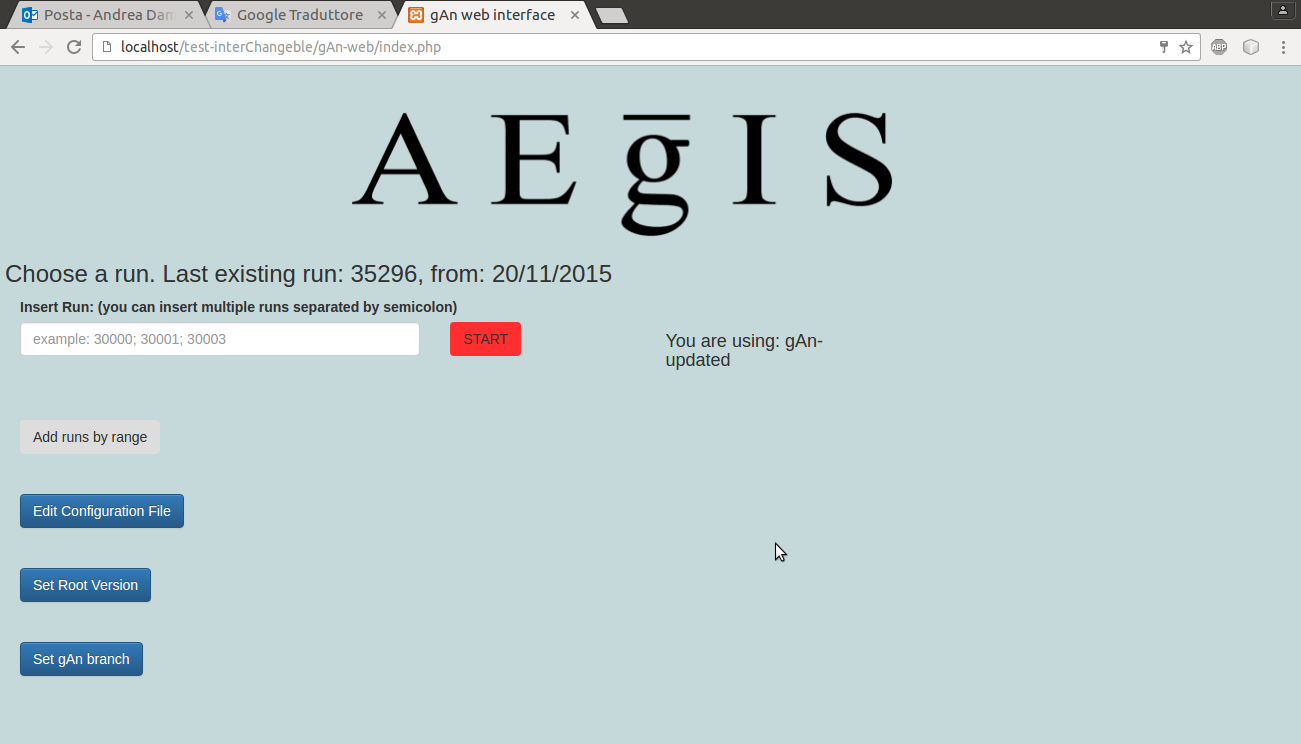
\includegraphics[scale=0.25]{HomePageEmpty.png} 
\caption{Intermediate version: the homepage of gAn Web without input}
\end{figure}


\begin{figure}[H]
\centering
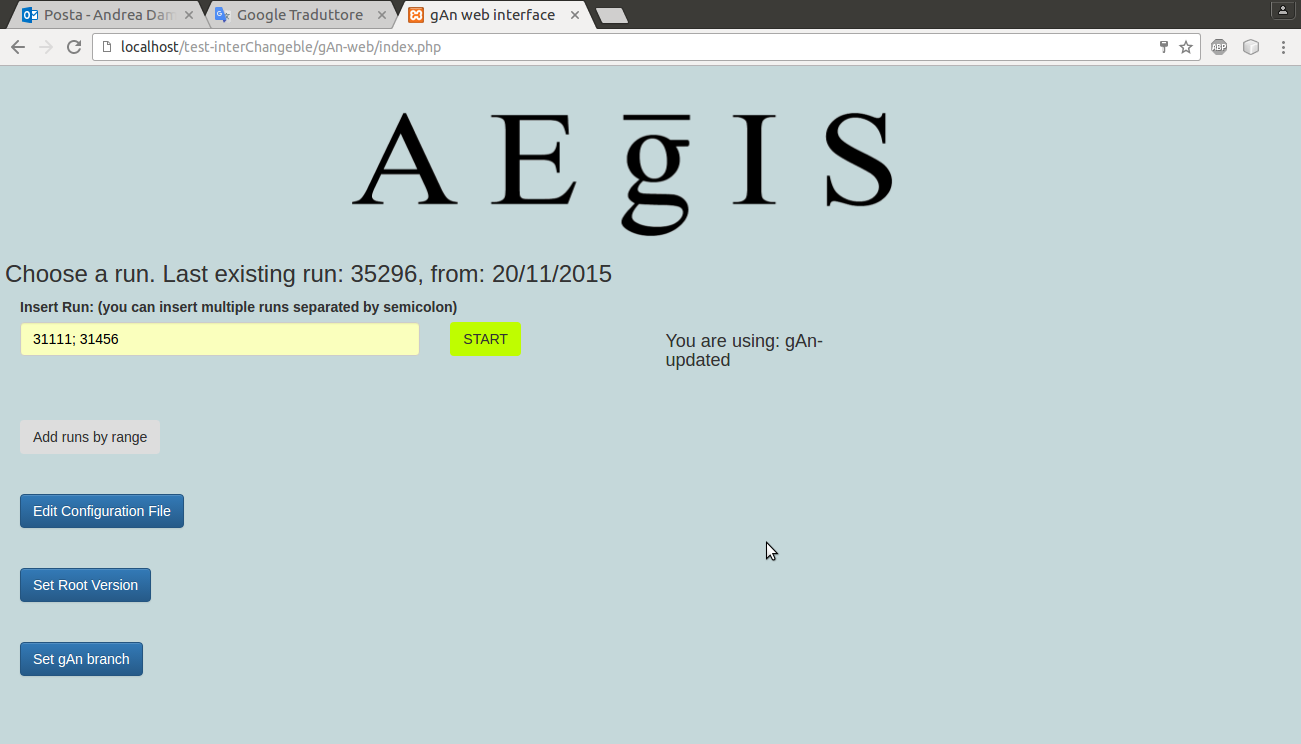
\includegraphics[scale=0.25]{HomePage.png} 
\caption{Intermediate version: the homepage of gAn Web ready to start}
\end{figure}

There are some modifications:

\begin{enumerate}

\item The user is informed about what is the last existing run: he can read "last existing run: nnnnn, from dd/mm/yy". This point is important because in most cases the user searches results regarding the lasts 2 runs.

\item The button named "send" was unclear, the word "START" is more clear, the user can immediately understand that the goal of this button is to start gAn. The button is red and disabled if there are problems (like in the following image) with the inserted runs (or if the input field is empty), green and clickable if there are no problems.	

\begin{figure}[H]
\centering
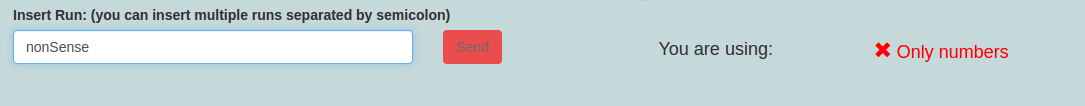
\includegraphics[scale=0.25]{ErrorInputHomepage.png}  
\caption{Intermediate version: the "Start" button is red if the values in the input field are invalid}
\end{figure}

When the user clicks start a progress bar appears. Unfortunately it is very hard to understand exactly how long the computation will last, because different runs can take different time (it depends on the amount of data that the sensors take about the run, and on the workload of the server machine, that is in common with other applications). On average has been observed that the computation takes five seconds multiplied by the number of selected runs, but there is a cache system. A wait of several seconds can be not acceptable for the user, the progress bar is imprecise but ensure to the user that the system is working correctly to ensure the correct answer. The problem is not solved: the wait time is still too long, but a solution in this case comes from the back-end, a re-factor of the code will soon make the wait time shorter. In the following image the progress bar:

\begin{figure}[H]
\centering

\includegraphics[scale=0.25]{ProgressBar.png}  
\caption{Intermediate version: the progress bar aims to make more accepttable the user's waiting}
\end{figure}



\item The input field has a place-holder, that shows to the user how to correctly insert the runs separated by semicolon (there is an automatic system that corrects the inserted values if the separator inserted by the user is not a semicolon)
 
\item It is possible to insert a group of runs selecting them by range (inserting the first and the last): the button "Add runs by range" opens a modal (shown in the image). The user can choose the minimum and the maximum value of the range, the system validates the inserted values (maximum must be more that minimum, they must be numbers etcetera).

\begin{figure}[H]
\centering
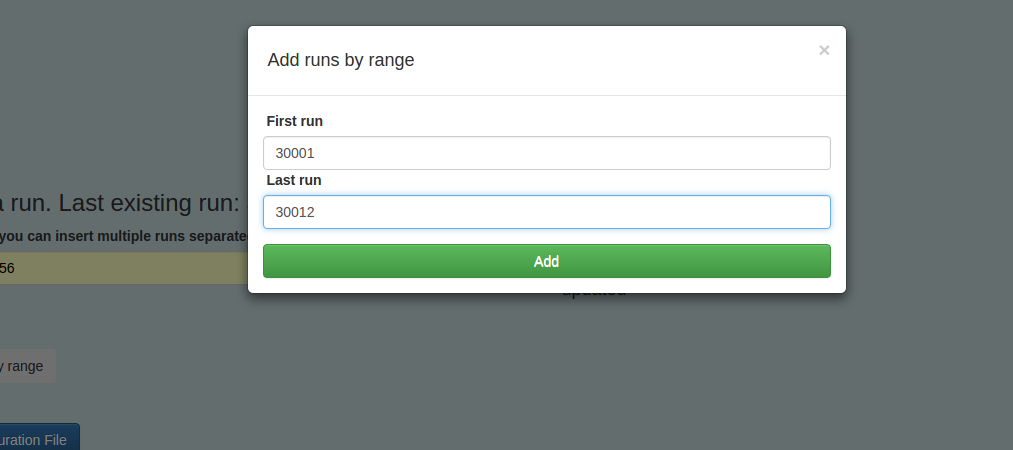
\includegraphics[scale=0.25]{RangeRunsModal.png}  
\caption{Intermediate version: the modal opened by clicking the button "Add runs by range"}
\end{figure}

\item There is a message "You are using: nameOfGAnBranch" that informs the user about which is the branch of gAn used. By default if the user doesn't change the configuration the used branch is the last used, in the last successful execution.

\item There are two new buttons: "Choose Root version", "Choose gAn version". These buttons redirect the user to pages able to modify the version of Root and gAn used in the computation.
 
\item Each button and each field have a tooltip: a text that appears when the user moves the mouse over the object. In this way an inexperienced user can easily understand what each component does.  

\end{enumerate}


The page related to the modifications of the configuration file of gAn is shown in the following:

\begin{figure}[H]
\centering
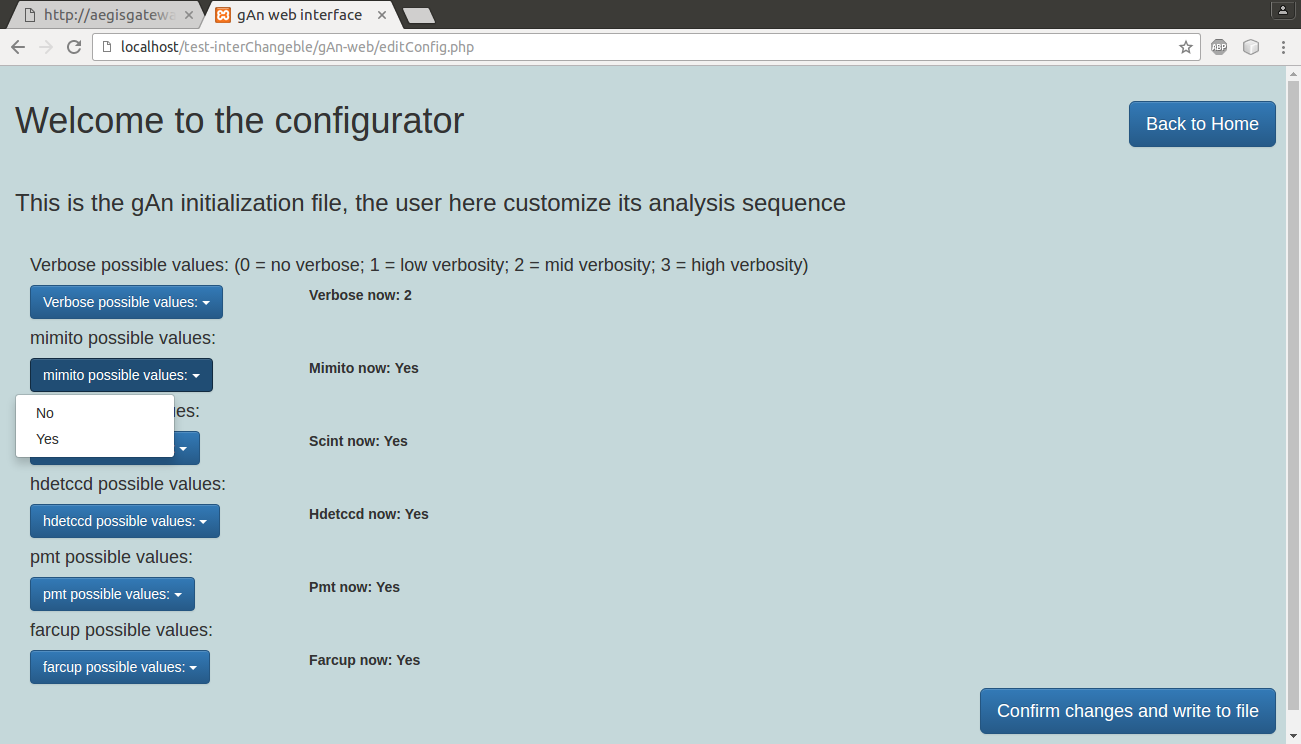
\includegraphics[scale=0.25]{EditConfig.png} 
\caption{Intermediate version: the edit-configurator page of gAn Web}
\end{figure}

This page doesn't use any more radio buttons, dropdown menus are preferred for aesthetic reasons. The user can read near the button the currently selected value for each field. 

\newpage

The page that shows the textual output of gAn is exposed in the following images, has some modifications:

\begin{figure}[H]
\centering
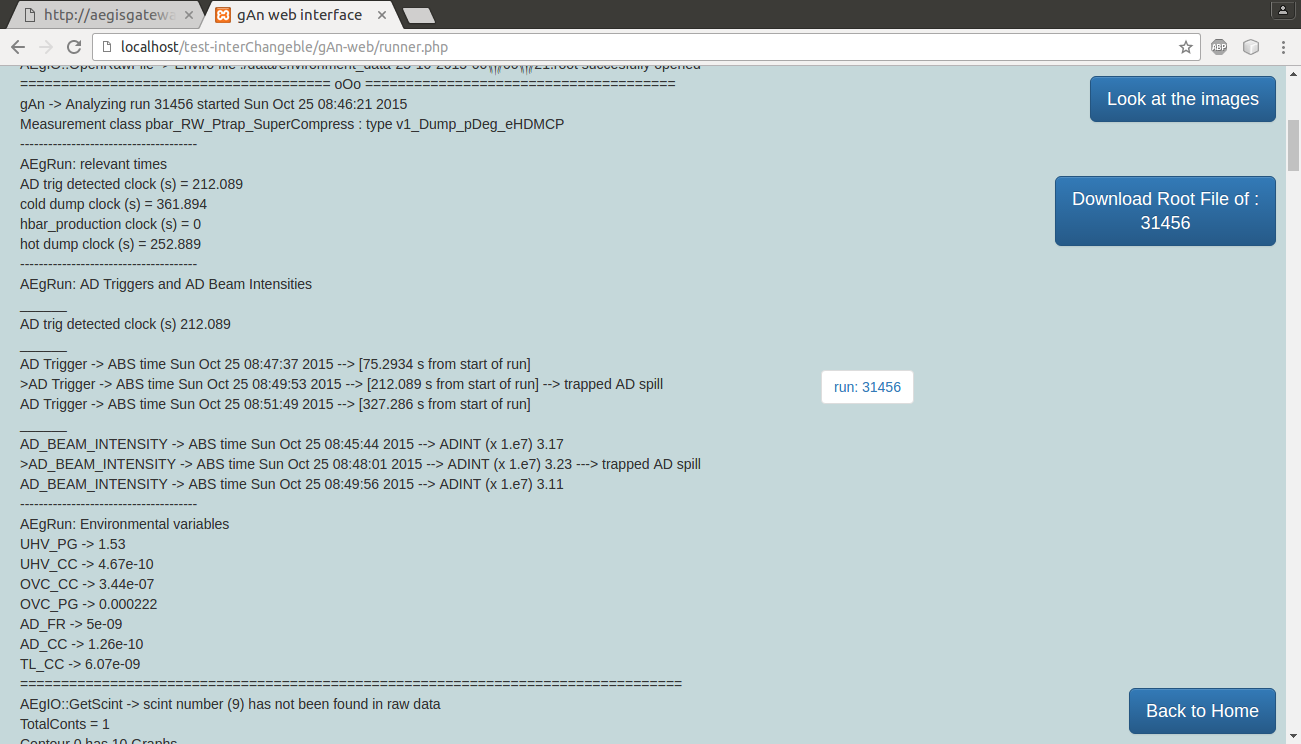
\includegraphics[scale=0.25]{TextOutputPage.png} 
\caption{Intermediate version: the page who shows the textual output of gAn}
\end{figure}


\begin{enumerate}
\item The user can choose what results he wants to show on the screen by clicking the corresponding run number from the "navbar", like in the image:

\begin{figure}[H]
\centering
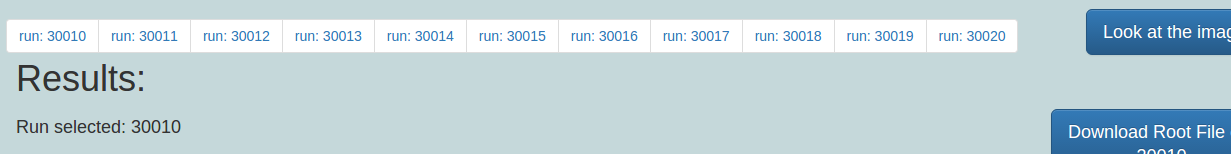
\includegraphics[scale=0.25]{WhichRunNavbar.png} 
\caption{Intermediate version: by this "navbar" the user can choose the run results to show}
\end{figure}

This navbar is in fixed position related to the screen, and can be dragged by the user to allow him to decide where put it.

\item "Download Root File of: nnnn" is a button that allows to user to download the semi-processed file .root with some output information regarding the computation.

\item "Back to Home" gives the user the opportunity to directly return to the homepage. 

\item "Back to Home" and "Look at the images" are in a fixed position on the screen: even if the user scrolls down or up the screen he is always able to see these buttons.    

\end{enumerate}
The page that shows in an organized way the images that gAn produces in output. The following image shows the new appearance of the page:



\begin{figure}[H]
\centering
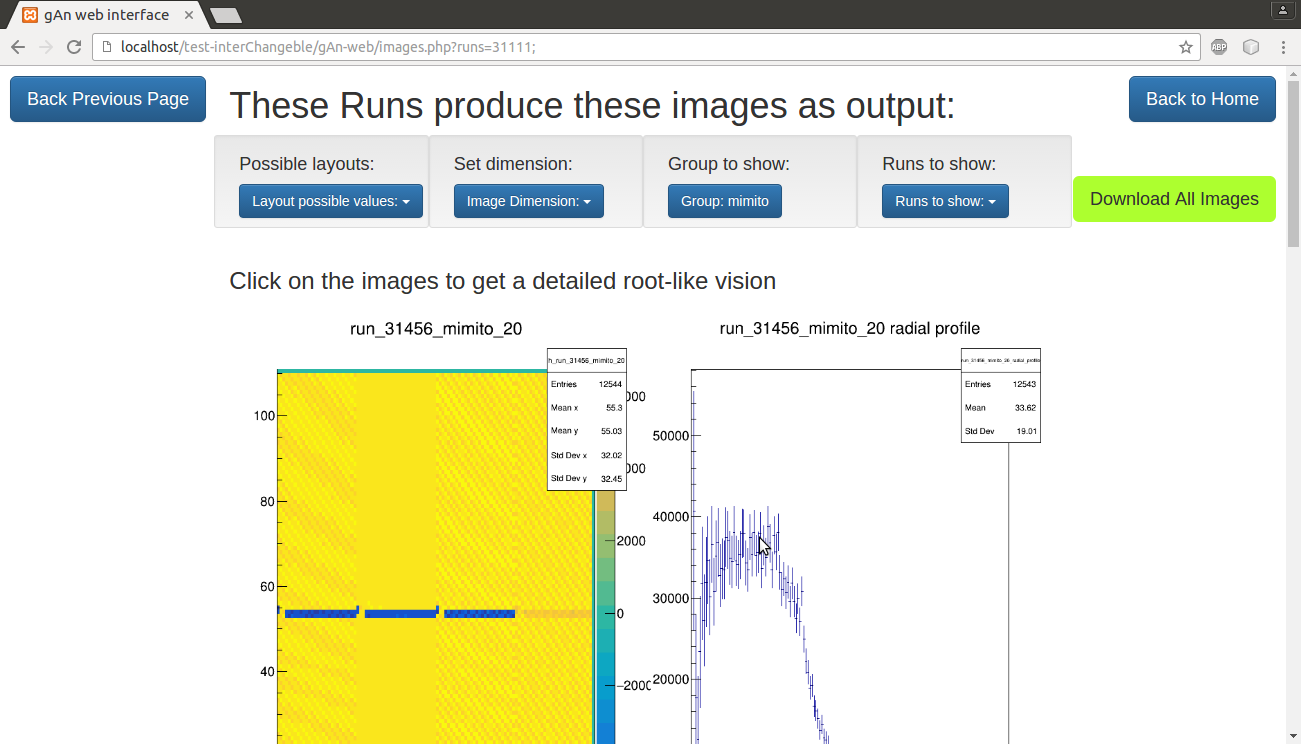
\includegraphics[scale=0.25]{AllImagesPage.png} 
\caption{Intermediate version: this page shows all the images that gAn produces in output}
\end{figure}


Modifications:
\begin{enumerate}

\item The dropdown menu "Runs to show" allows the user to select only the images produced by a single run (by default the system shows the images related to all the runs). The users widely use this option, because in this way they can compare images extrapolated in the same way but related with runs with different configurations.

\item "Download All Images" allows the user to download by a single click all the images related to the execution. The intermediate version introduces this requirement because commonly the users download the images using the right click of the mouse and the browser's button "Save Image As". In this way this process is faster and easier.

\item The buttons "Back to Previous page" and "Back to Home" are links towards the textual output page and the homepage. They are in fixed position.

\item By clicking on the image the user reaches a page that shows the image in full screen, but not in a static format: the image is dynamically accessible like shown in the following images:

\begin{figure}[H]
\centering
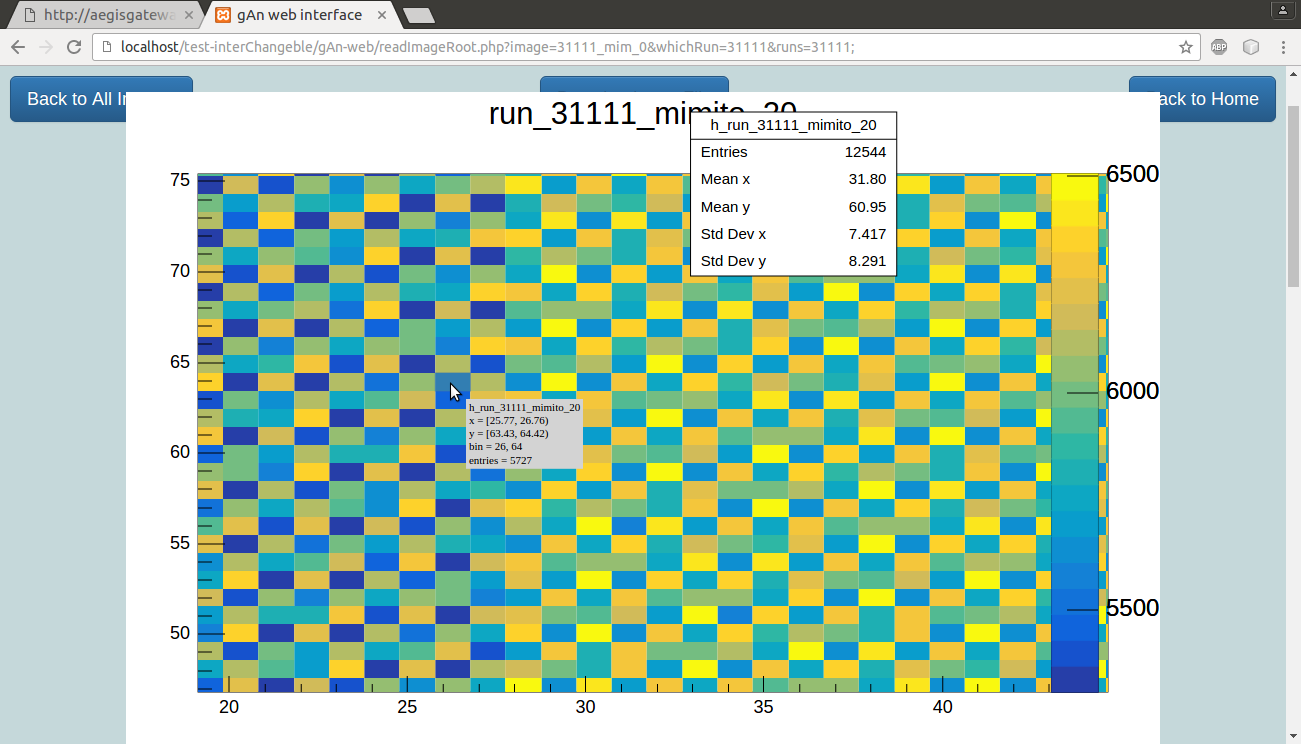
\includegraphics[scale=0.25]{RootLikeImage2.png} 
\caption{Intermediate version: moving the cursor the system shows the value of this histogram in the selected point}
\end{figure}



\begin{figure}[H]
\centering
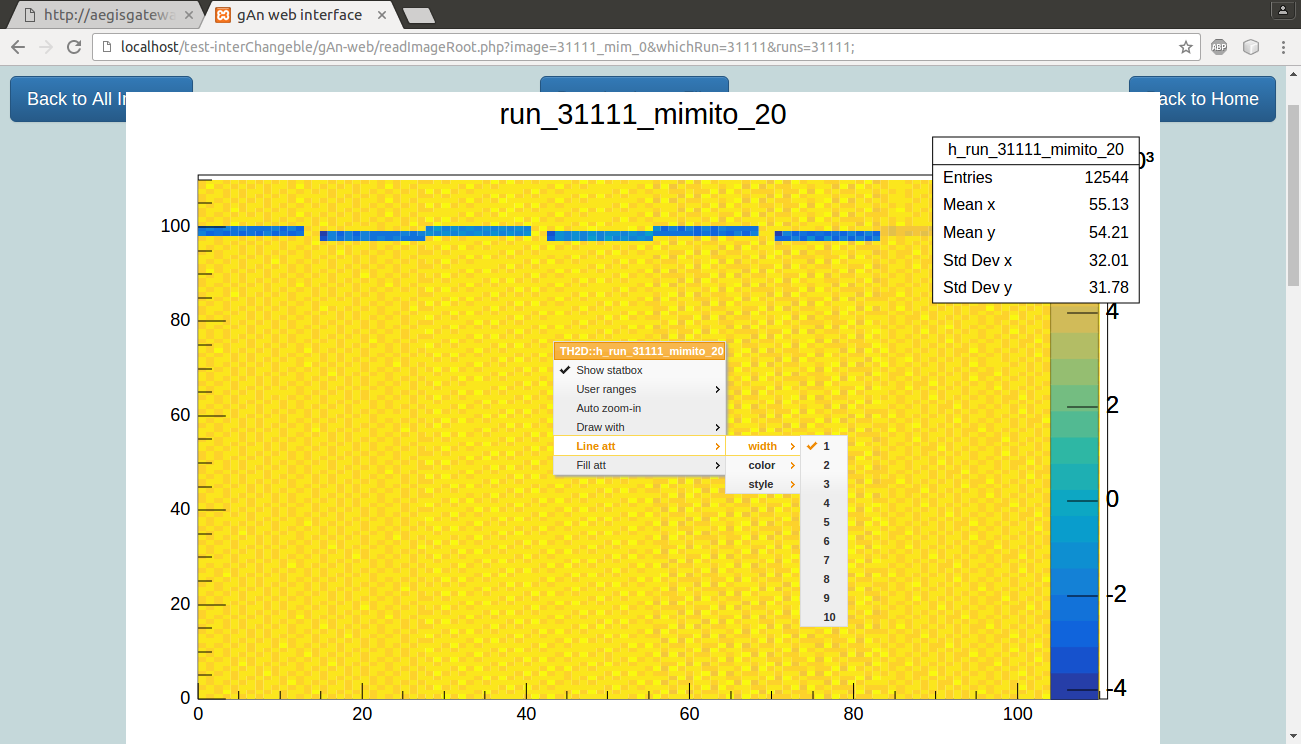
\includegraphics[scale=0.25]{RootLikeImage.png} 
\caption{Intermediate version: the user can modify numerous settings in the generated image}
\end{figure}

\begin{figure}[H]
\centering
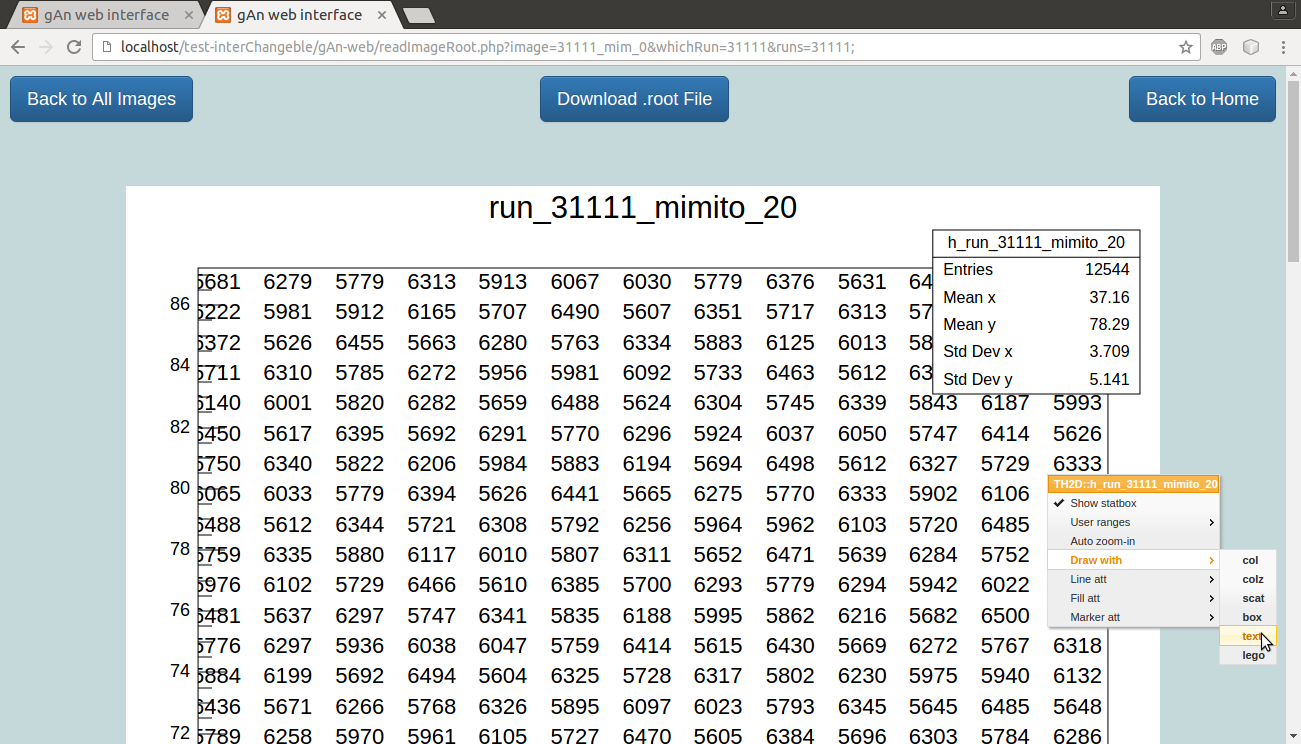
\includegraphics[scale=0.25]{RootLikeImage3.png} 
\caption{Intermediate version: the user can show the histogram not only in traditional format, but also in a numerical format where the numbers are the value of the function in their position}
\end{figure}

\begin{figure}[H]
\centering
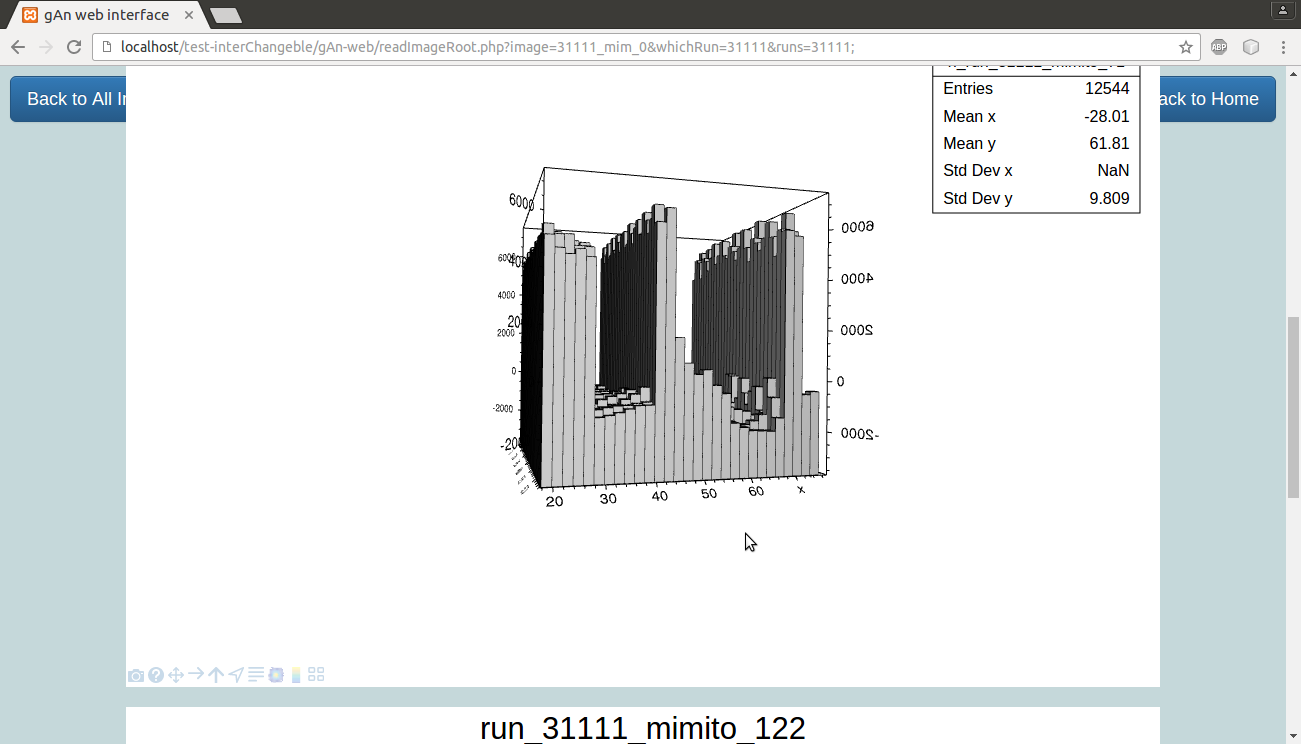
\includegraphics[scale=0.25]{RootLikeImage4.png} 
\caption{Intermediate version: another solution is to generate a 3d image in lego-style of the histogram}
\end{figure}


 
\end{enumerate}


\subsection{Added pages}

Some pages in the intermediate version are completely new, because they implement new functionalities.

The first new page that the user sees is the login page. It is very simple, it doesn't authenticate a single user, but asks only the password of the office. This basic system of authentication aims simply to ensure that only the people that works in AEgIS experiment can use this software.

Following the login page image:

\begin{figure}[H]
\centering
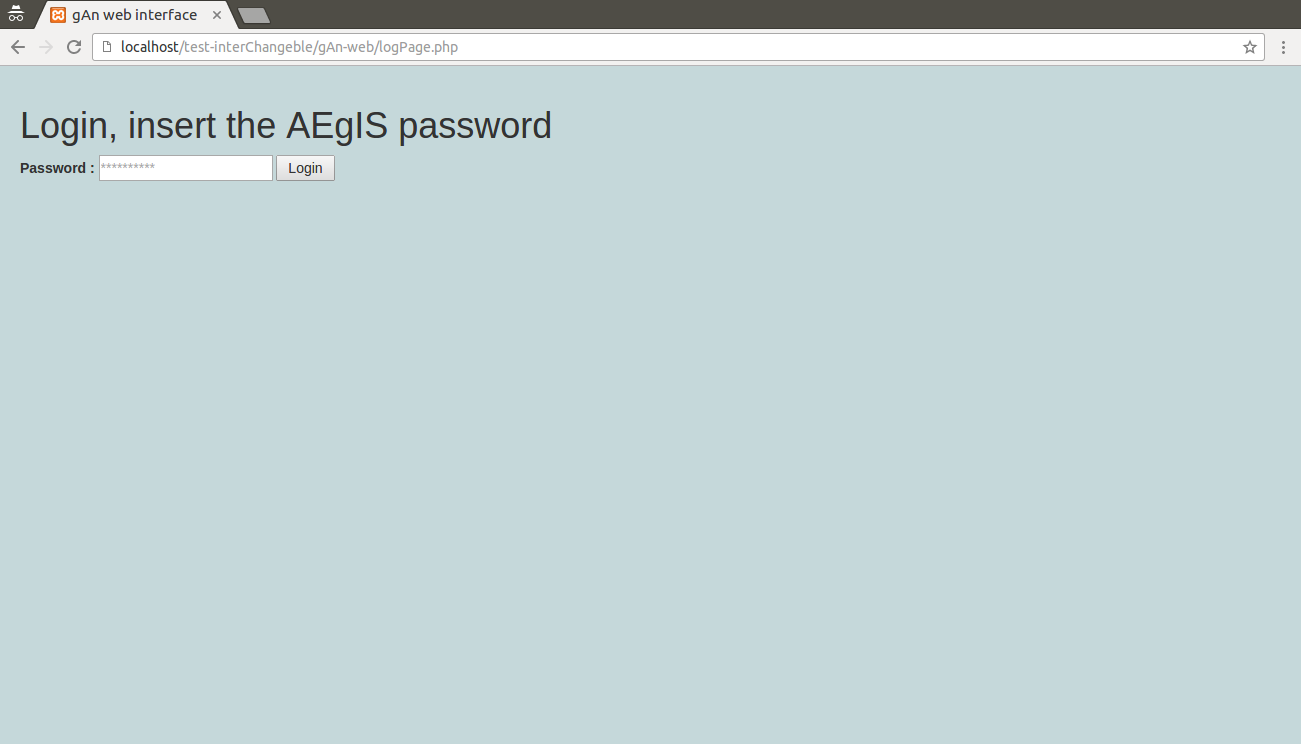
\includegraphics[scale=0.25]{Login.png} 
\caption{Intermediate version: simple login page}
\end{figure}

In this version there is also the opportunity for the user to choose which branch of gAn and which version of Root Framework to use to execute the program. The pages that the user can user are quite similar, and quite simple. The user must use dropdown menus to make these choices, and there is always a default safe choice (the system remembers the last working version of Root and the last working branch of gAn), so it is impossible make errors or inconsistent choices. 

Following there are some screen-shots of these pages

\begin{figure}[H]
\centering
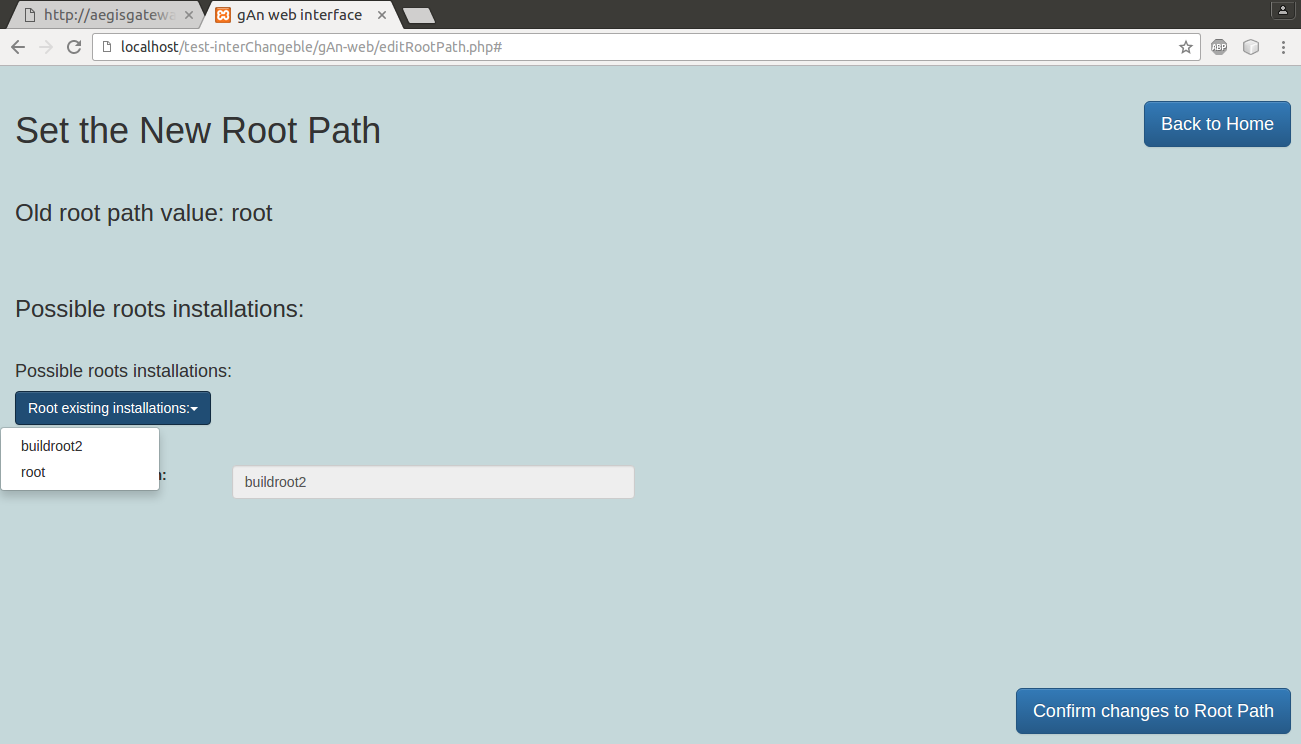
\includegraphics[scale=0.25]{RootVersionChoice.png} 
\caption{Intermediate version: page where the user can choose the Root version to use}
\end{figure}
 
 
\begin{figure}[H]
\centering
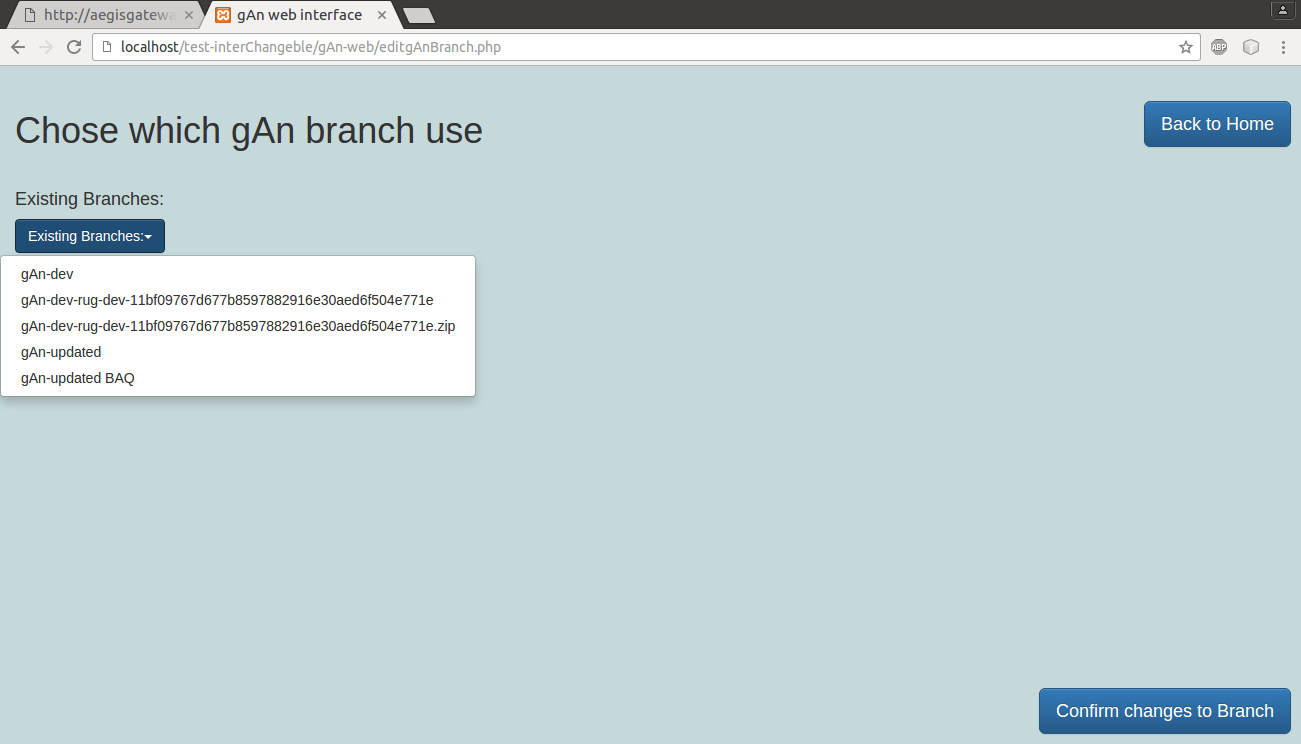
\includegraphics[scale=0.25]{ChoosegAnBranch.png} 
\caption{Intermediate version: page where the user can choose the Branch of gAn to use}
\end{figure}

% Chapter 6

\chapter{Final version} % Main chapter title

\label{Chapter6} % For referencing the chapter elsewhere, use \ref{Chapter5} 

Here the features of the final version will be explained. This version is very close to what we want to create as final application.

\section{Functional requirements}

The last version (thereafter "gAn Web v3") is a modified version of the intermediate version. 
The changes with respect to the second version come from two sources: some additional requirements and modifications are proposed from the super users and some else come from the tests made with the generic users; 
The first group of adding requirements (the ones proposed by the supervisors) are the following:

\begin{enumerate}
%1 choose analysis new way
\item 
The main kinds of analysis are now more clear: they are around 10, their goals, so their input as well as their expected output are quite stable, although we will still probably modify the algorithmic ways in which these goals are achieved. Their roles and when they are useful is now steadily fixed (more precisely: we are pretty sure about the role of the existing analysis, but in the future we can add more analysis..). Each user, according to his task, knows (should know) in every moment which analysis fits better the situation, so, the best solution is to allow the user to choose the type of the analysis through a dropdown menu directly in the main page (exactly like he chooses the run number). To make the user's life easier the application can use a tooltip for each analysis, to remember him in which situation it is useful. At this point the possibility of choosing the gAn version is useless, because the final version of gAn include all the existing types of analysis. 

%2 single vs multiple
\item 
The kind of use of this software is quite different if you decide to work with a single run or a group of runs, so it is better if at the beginning (at the application starting) the user chooses directly if he wants to work with a single run or more than one. 

Therefore the application becomes modal: we hope that the simplicity of the interaction and the presence of a box that constantly informs the user about which "mode" he is using can reduce confusion instead of let it grow.  

If the user works with a single run the focus is mainly on the "exploration" of the information in the data, with the multiple runs the focus is more on the possibility to compare and see what is different.

In the second case (more than one) it is better to specify if the runs are a range (from N to M, all the runs between) or a group of non-consecutive runs (it can be useful, because of the feasibility to compare non-consecutive runs can be interesting). If the user is interested in a group of runs that are not a range (we observe that this situation is not common, but we must manage it), the previous solution of multiple runs separated by a comma is not a good idea: often in these cases the searched runs are little consecutive groups, so a list of ranges. It is better if the user can have an input area (like a sheet) in which he can put the intervals, divided in different lines (or other separators).

%3 don't choose root version
\item
There is an effort in the developing of the whole project to make it independent of the Root version, so the interface won't ask to the user to choose a Root version anymore. 

%4 need to be quite aesthetically acceptable
\item
The aesthetic part in this application was neglected in the first and intermediate versions, but now it needs to be cured and improved to ensure the best possible satisfaction to the users. 

\end{enumerate}
 
Furthermore, the version with this last requirements was tested with the users: the developer studied their behavior observing them at work with the existing version, listening to their comments, and asking them opinion. The impact of the debut with the users highlights some problems to be overcome, and also provide some interesting ideas: from the analysis and the solution of these problems and from the user's proposals the requirements of the last version has been defined. 

In chapter 7 (\ref{Chapter7} ) we will explain how the tests with the users took place and what are the results.

The main problems observed (and for each the proposed solution) are the following:

\begin{enumerate}
\item 
It is important to help the user in some way to choose the run number: the user needs a view on the logbook of the run, that is a text in which there is information about each run number grouped by date.

\item
Actually nobody use the button to modify the dimension of the images: they all use the biggest version.. therefore it is better to remove (or move in a less central place) this dropdown menu. A similar reasoning can be done for the dropdown that allows the user to switch between the vertical and carousel menu (everybody use vertical, clearly at this point the carousel version isn't useful). Also nobody use the run selector to choose which image see: their choice relies on the image's title.. this means that the existing navbar is not suitable to satisfy the needs of the user, a better solution is to create a selector with the image's titles, specifically a group of check-boxes, each with the title of an image as label.  

\item
The read of the textual output takes too much time: it can be improved highlighting the most important parts (or better, the most important parts for the selected type of analysis)

\item
The user needs to choose by the configuration page the degree of precision (the minimal error) of the x-axis (the time related axis) of each time-related values images. This parameter seemed to be not very important and in the second version actually there was removed, but almost all the users modified it quite often (manually), and verbally asked for the possibility to set it through the interface. So it is better to let them to introduce this parameter by setting it through the interface.

\item
The general organization of the output is simply, but not the best possible: the users need to switch easily from textual to images output and vice-versa, and the buttons are too many spread on the screen, so too difficult to find.

\end{enumerate}

\section{Non-functional requirements}

There is another special requirement emerged in this version, not strictly related to the common behavior of the interface but quite important: the machine  used as server is also used for the testing of single analysis when they are written; sometimes these analysis crash (quite normal in a test phase), and they remain in a "hung up" state, without doing nothing but occupying Ram memory, and if the blocked application are numerous that can be a problem for the performances of the machine. To ensure a correct behavior gAn Web must check this situation at starting and eventually resolve it.

\section{Scenario--based functional analysis}
Following we can show some examples able to explain how the typical interaction must work in the final version:

\begin{enumerate}

\item
Let's suppose a very common situation in a shift: 
In the work-shift the run NNNN is running. The shifter wants to calculate the temperature of some particles with a (complex) process based on the shape that they create on a sensor. The basic idea is: if a particle is hotter, its speed is bigger, it can escape more easily from a magnetic trap, and the sensor can observe more particles outside the trap. At this point the software tries to fit, with an exponential function, the shape of the signal that the sensor shows as output, and through the integral of the slope of this exponential function can estimate the temperature of the particle.
The user chooses the single analysis, inserts the run NNNN, selects the kind of analysis called "TemperatureMeasurement", clicks the "start" button;
The system shows to the user a textual output and some images: 
The textual output proposes a lot of information, but in most cases the user is interested in only three parameters, that are clearly highlighted by a special font, a color and a visible border. 

The user must also check the image: there is the histogram of a signal, an a red line where the function is fitted. The user checks if the red line
has an exponential shape (if it is a straight line the situation is too aleatory and the data are not affordable); the user also checks if the fit line is too long (it must be very little to accept the results of the analysis, because of physical reasons). 

Let's suppose that the fit function is a straight line: the user can retry the same analysis with a different setting: he returns to the homepage (through the button "New Analysis" on the Navbar), he clicks "Advanced Settings" to modify the configuration, he inserts a new value through a slider, to have a more precise graph, in the hope to fit it better. At this point he can retry the previous algorithm (a more precise function will lead a slower computation but probably will give an affordable output)  

\item 
The user is interested in two distinguished groups of runs, from 57001 to 57005 and form 57016-57020.
This situation is very common because most of the groups of measurements are repeated in two different slices of times (to be sure about the results).
In this case the user, after having selected "Multiple runs", can click on "By InputArea" and a text area appears. In the area there is the value inserted the last time that the user used this function (we observe that it is quite common to repeat analyses with the same groups). The input is quite free: user can insert a group inserting the first and the last separated by a dash, a space, or a comma, and other group by changing the line (so each not empty line is a group). 
The user at this point selects the analysis and runs the program. 

\item
The user is interested in a range of runs, from 58001 to 58010, to perform the same analysis and check if and how some values are varying. He can select multiple runs, insert the first and the last, select the analysis (the multiple runs analysis are taken from a different set from the single runs analysis).

\item
The user inserts a run, and selects an analysis names PMTs. This kind of analysis takes information from a group of sensors and produces in output (usually) seven images. The user often is not interested in all the seven images but in one or two. At this point, using the check-boxes selector he can select/deselect images to show (by default they are all selected).  

\end{enumerate}

\newpage
\section{Prototyping - Implementation}

Here is explained with some screen-shots how the final version looks like, and how does it work.

Login page:


\begin{figure}[H]
\centering
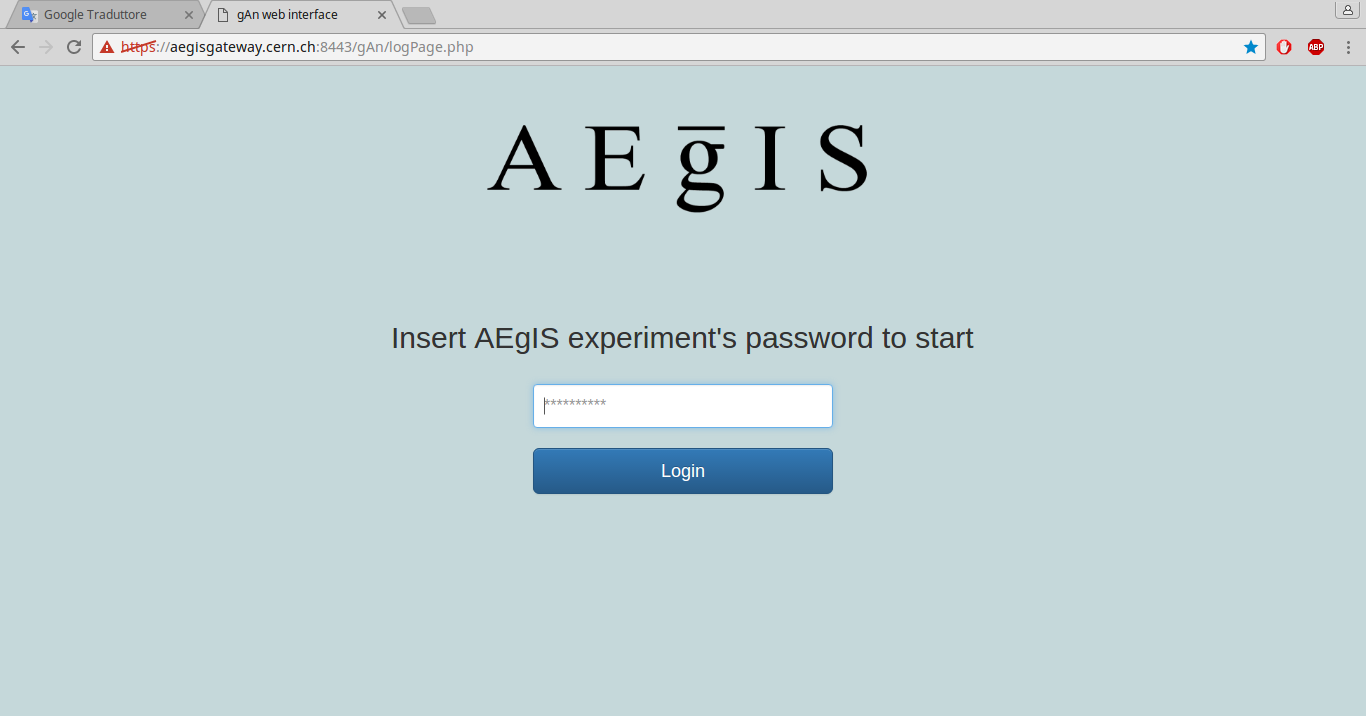
\includegraphics[scale=0.25]{LastLogin.png} 
\caption{Final version: the Login Page of gAn Web}
\end{figure}

First of all the login page: it is very simple, only one user exists (all the people in the AEgIS experiment are equal when they use this software, and no others experiments use this application) so only the password needs to be inserted, in order to ensure that only people who work in the experiment can use the software. We can see the typical objects taken from the Bootstrap's default graphic objects.

\newpage

Home page, initial choice:

\begin{figure}[H]
\centering
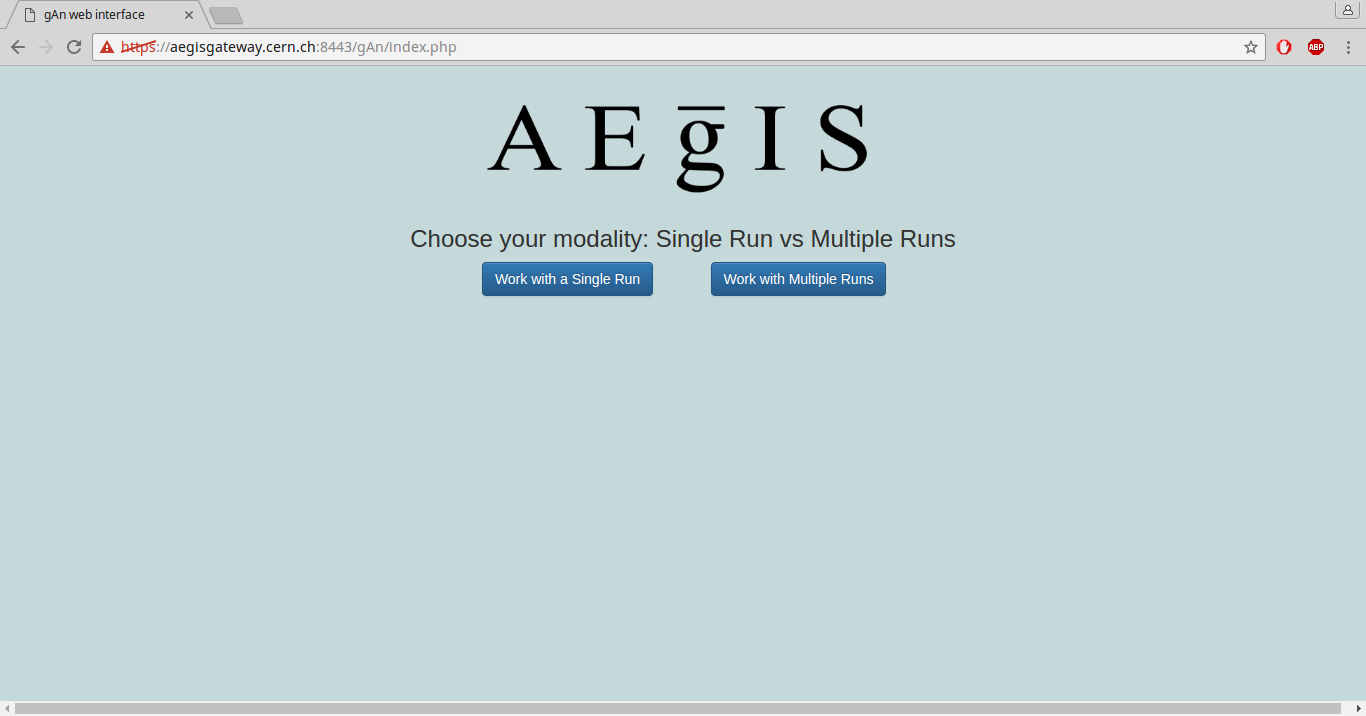
\includegraphics[scale=0.25]{LastInitialChoice.png} 
\caption{Final version: the first thing that a logged user sees}
\end{figure}
  
The neo-logged user can here choose if he is interested in a single run analysis of in a multiple runs one. These two situations are quite different, so the application works with them in two different ways.

After the choice, the user can always change idea, by the appropriate button:

\begin{figure}[H]
\centering

\includegraphics[scale=0.25]{ParticularExitStrategy.png} 
\caption{Final version: how the user can change his choice}
\end{figure}

\newpage
Home page, differences between single and multiple runs:

Here we can see how the two modalities of work (single and multiple) appear.

Single run: 
\begin{figure}[H]
\centering
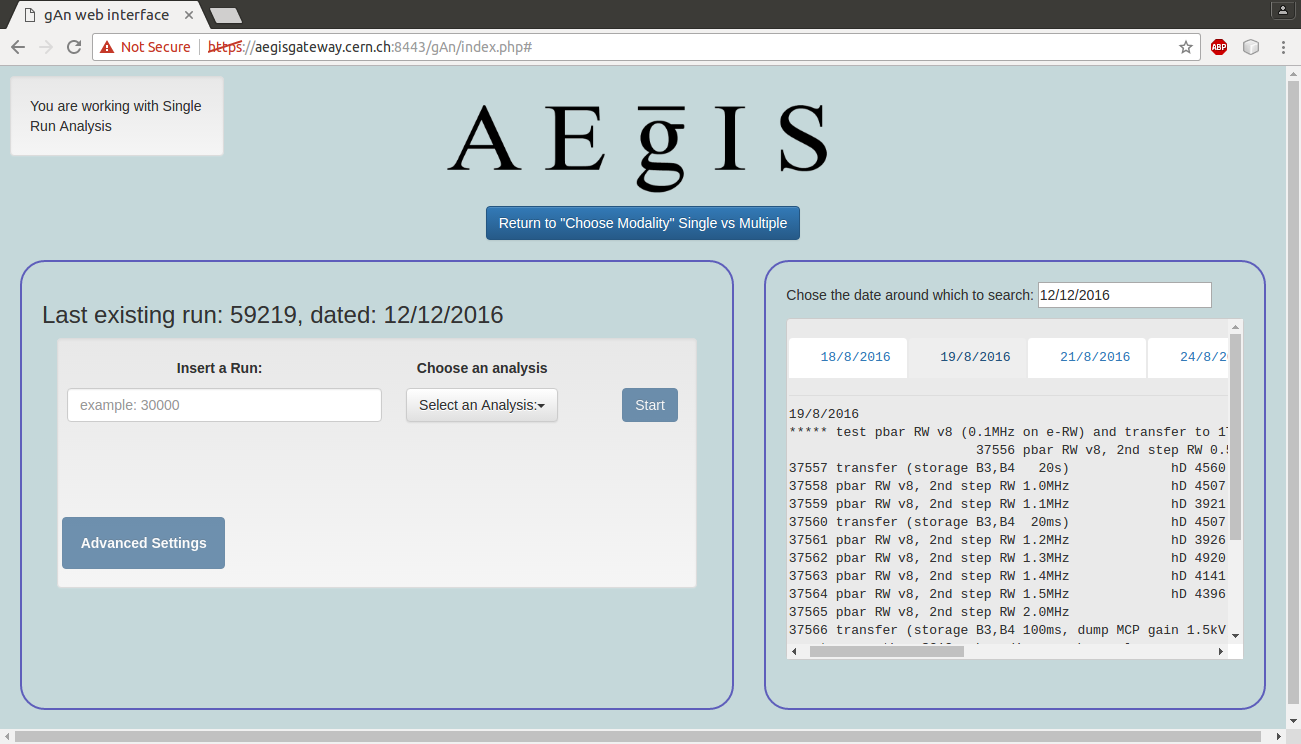
\includegraphics[scale=0.25]{LastSingle.png} 
\caption{Final version: the Homepage if the user chooses Single run analysis}
\end{figure}

the single one is more simple, on the left of the screen the user inserts a run number and a kind of analysis. We can see the button related to access the configuration page and modify the settings (Advanced Settings). On the right part of the screen there is a view on the RunLog of the experiment. The user uses the right part when he wants more information about what run use to work (actually this situation is quite seldom). In the case the user can insert a date using a datepicker, the system opens some pages related to the days around that date and in each page shows the content of the logs related to this date. The goal of the datepicker, provided by Bootstrap, is to reduce the charge on the memory of the users (it shows as default the current date, and shows as result the pages of the RunLog related not only to the selected date but also to the days before and after, to give the user some references and allow him to make errors of 2-3 days still finding the result) and to allow him to insert the date in a correct format. The logs are always divided in runs, and for each run there are some information and comments. At the moment this functionality is a mock-up (it is one of the few  mock-ups exposed in this document). 

On the top-left of the screen there is always a little note with some information about the status of the program: this is a little cognitive aid:


\begin{figure}[H]
\centering
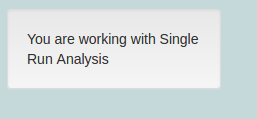
\includegraphics[scale=0.45]{ParticularStatusHP.png} 
\caption{Final version: a label with some information about the current status is always visible in the homepage}
\end{figure}    
 


On the screen there is always written the last known run, because in most cases the users use it or the immediately previous one. 

The interface informs the user if he makes some errors inserting the input. On the first implementation the error messages was programmed to became visible every time the inserted value was incorrect, so also at the moment the user was entering in the page and still hasn't inserted the values. This behavior is quite aggressive and unkind to the user.. it is surely not our intention so is a better solution if the error messages appear only when the user try to click send without having inserted correct values. The messages are hopefully aimed to explain the user how to solve the problem:

\begin{figure}[H]
\centering
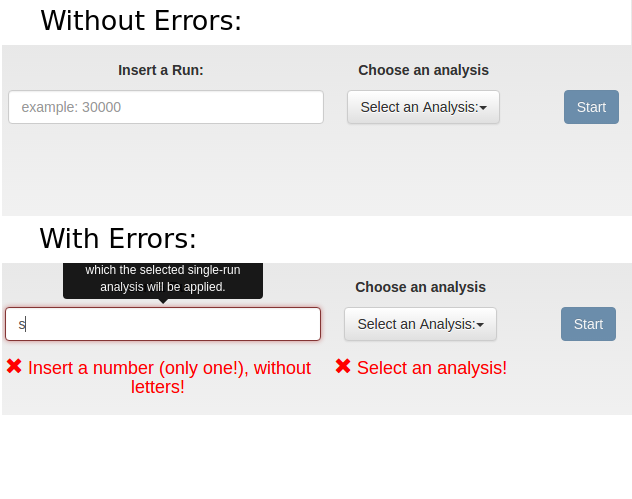
\includegraphics[scale=0.5]{ParticularHowErrorsWork.png} 
\caption{Final version: how error messages work}
\end{figure}    


\newpage
The dropdown menu usable to choose the kind of analysis is quite long (up to 10 options). A good idea is to order it and organize it in homogeneous groups:

\begin{figure}[H]
\centering
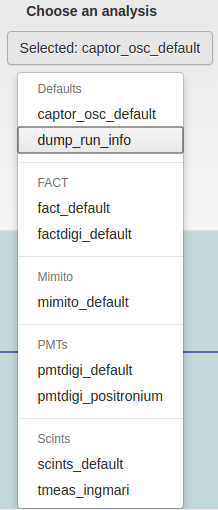
\includegraphics[scale=0.5]{ParticularDropDownSpecial.png} 
\caption{Final version: grouped dropdown menu}
\end{figure}    

  
Multiple runs:  
There is two different ideas about how to implement this page, because the new requisite about the fact that now the user can choose if insert one or more range using two input fields (for the first and for the last run) or a more flexible (but less efficient) "text area" is different from the previous version . So two different solution are evaluated, for convenience in this paragraph they are called "first" and "second", where the second is the correction of the first. So the first one was used to understand if the functionality is useful, the second one is a correction to ensure a more clear and better organized interface. At the end the second is the only one adopted in the application.

\newpage

Multiple runs first version:
\begin{figure}[H]
\centering
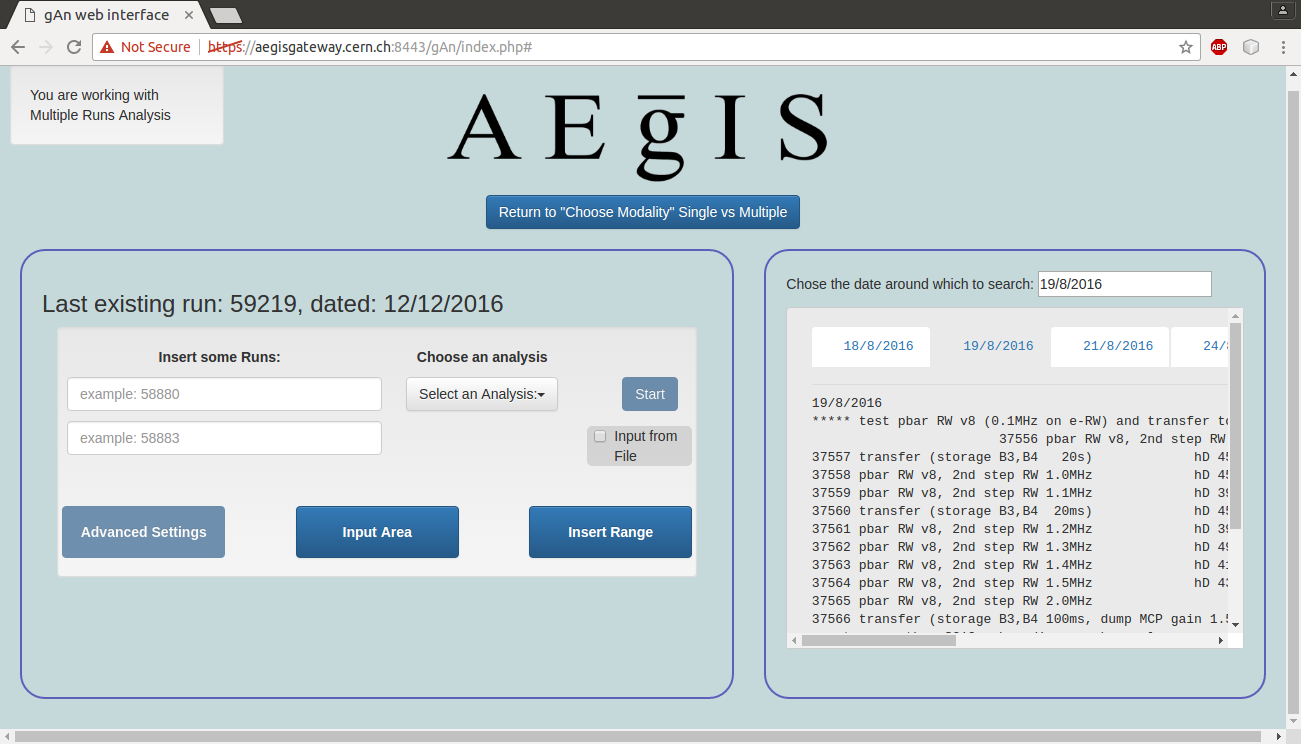
\includegraphics[scale=0.25]{LastMultipleFirst.png} 
\caption{Final version: the Homepage if the user chooses multiple runs analysis (first implementation)}
\end{figure}    

The multiple runs modality is similar to the single run but more complex: in a standard situation the user inserts two runs, the first and the last. The alternative (less used) situation is the one in which the user, through the "Input Area" button inserts a list of groups of runs (these runs are written in a file, that the system is able to accept as input). This modality is sometimes useful, and can be activated with the check-box "Input from file". The activation of this modality denies the access to the two input fields (you must only one way to insert runs..).
Following a little example of how the user can insert data through an Input Area in the first version:

\begin{figure}[H]
\centering
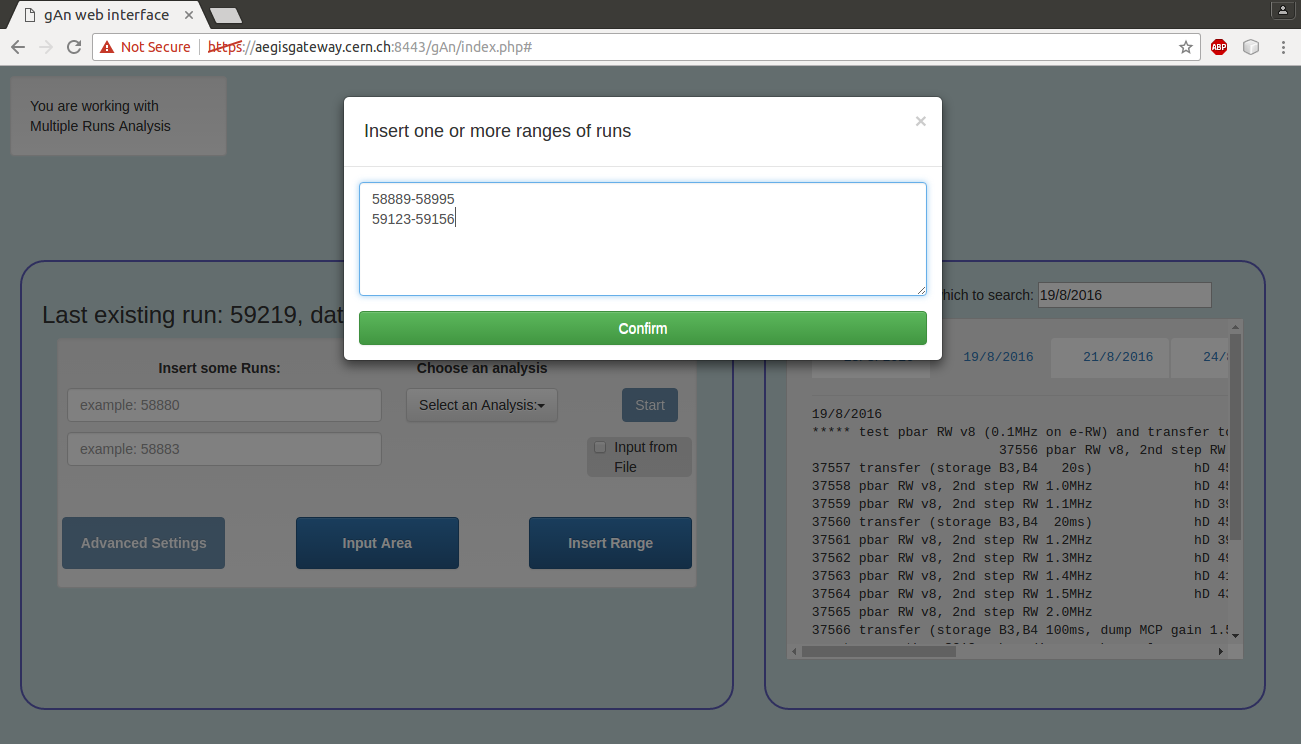
\includegraphics[scale=0.25]{LastMultipleRange.png} 
\caption{Final version: modal using which the users insert different ranges of runs (first implementation)}
\end{figure}   

Multiple runs second version:
The differences are only related to "how" the users can access the input field and the text area, the back-end is the same. Now the user can through a switching selector select which way he wants use to insert the runs. Obviously the selection of one way hides momentary the other one:

\begin{figure}[H]
\centering
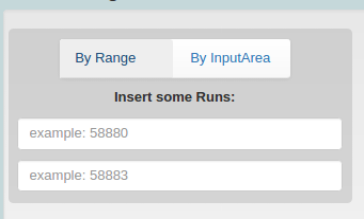
\includegraphics[scale=0.25]{ParticularRange.png} 
\caption{Final version: here is if the user selects "By Range" (second implementation)}
\end{figure}   

\begin{figure}[H]
\centering
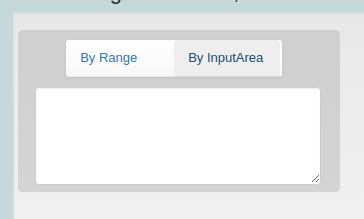
\includegraphics[scale=0.25]{ParticularInputArea.png} 
\caption{Final version: here is if the user selects "By InputArea" (second implementation)}
\end{figure}   

Now the little check-box near the start button is no-more useful (actually it created confusion), like the "Input Area" button. The interface is now more clear, without modals, with fewer commands but able to do the same things. A well surrounds the "runs related" part of the input system that now is quite composed and needs to be perceived like a "group".
Following how the multiple-runs interface appears now:

\begin{figure}[H]
\centering
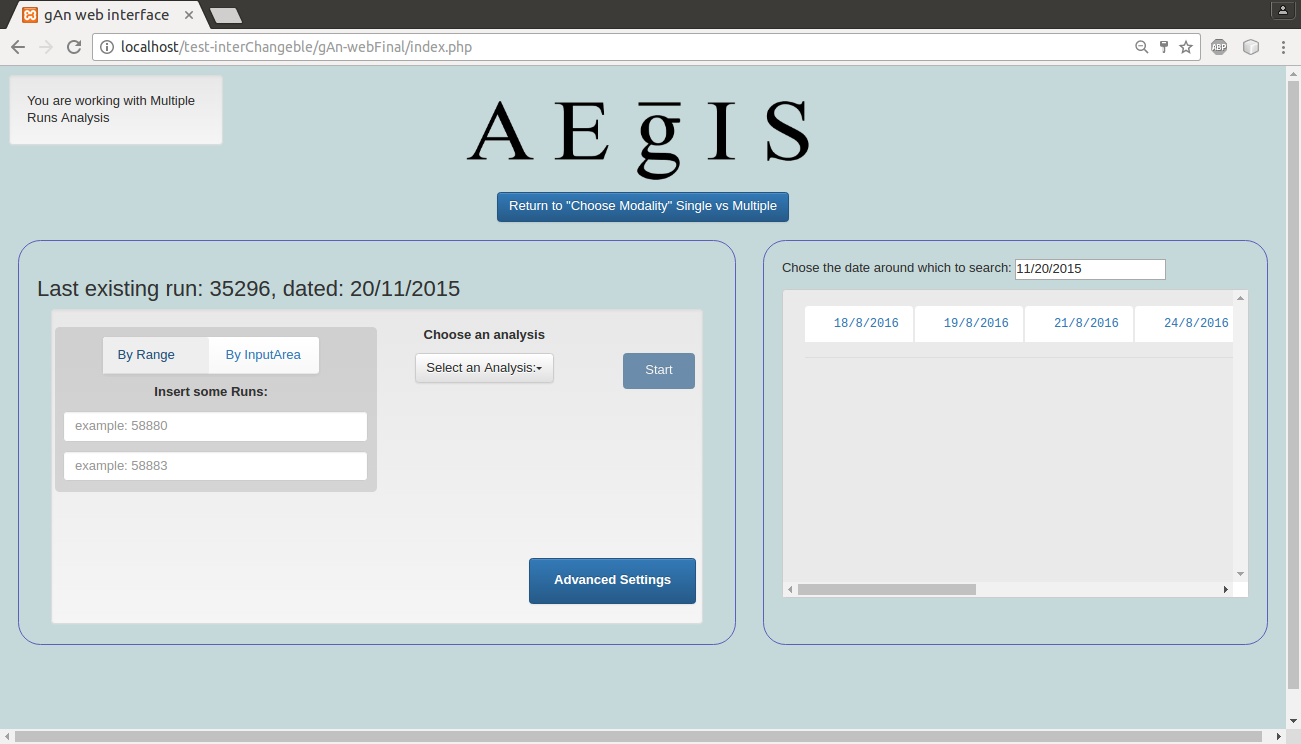
\includegraphics[scale=0.35]{LastMultipleSecond.png} 
\caption{Final version: how the homepage appears (second implementation)}
\end{figure}  

Advanced Settings page:

\begin{figure}[H]
\centering
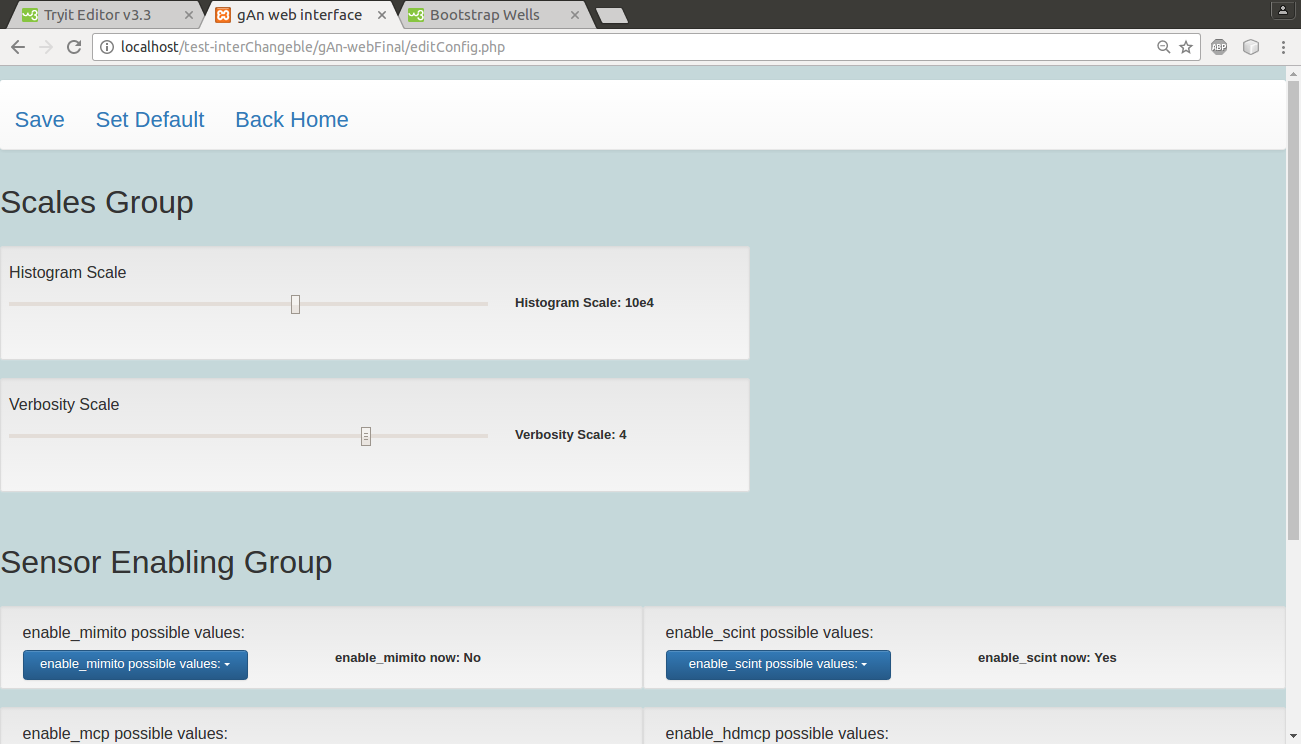
\includegraphics[scale=0.25]{LastEditConfig.png} 
\caption{Final version: the page related to edit configurations}
\end{figure}   

This page aims to allow the user to modify some groups of settings. The general rule is to use dropdown menus if the choice is true/false or Yes/No (	quite common) or between a reduced number of textual options, an to use instead  seekbars (an input bar moving which the user can insert a bigger or smaller numerical value) when the user must set a numerical value that goes from a minimum to a maximum value. On the top of the screen the user chooses to save the current setting, to return to the default setting, to go back home (without saving).    

In some cases the values to insert by the seekbars are in a very big range and is not easy to the user to have a too long seekbar. A good solution is to choose an exponential values seekbar: so the user chooses the exponentiation, not the number. This choice is quite reckless for normal users.. but for physicists the understanding of how an exponential value works is not a problem:

\begin{figure}[H]
\centering
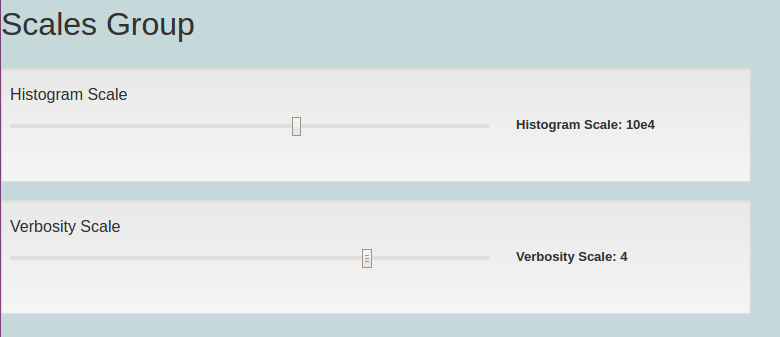
\includegraphics[scale=0.25]{ParticularScalesExpo.png} 
\caption{ Final version: an example of exponential scale (the first) followed by a non-exponential scale (the second) }
\end{figure}  

\newpage

Other setting are more easily accessible by some yes/no dropdown menus:


\begin{figure}[H]
\centering
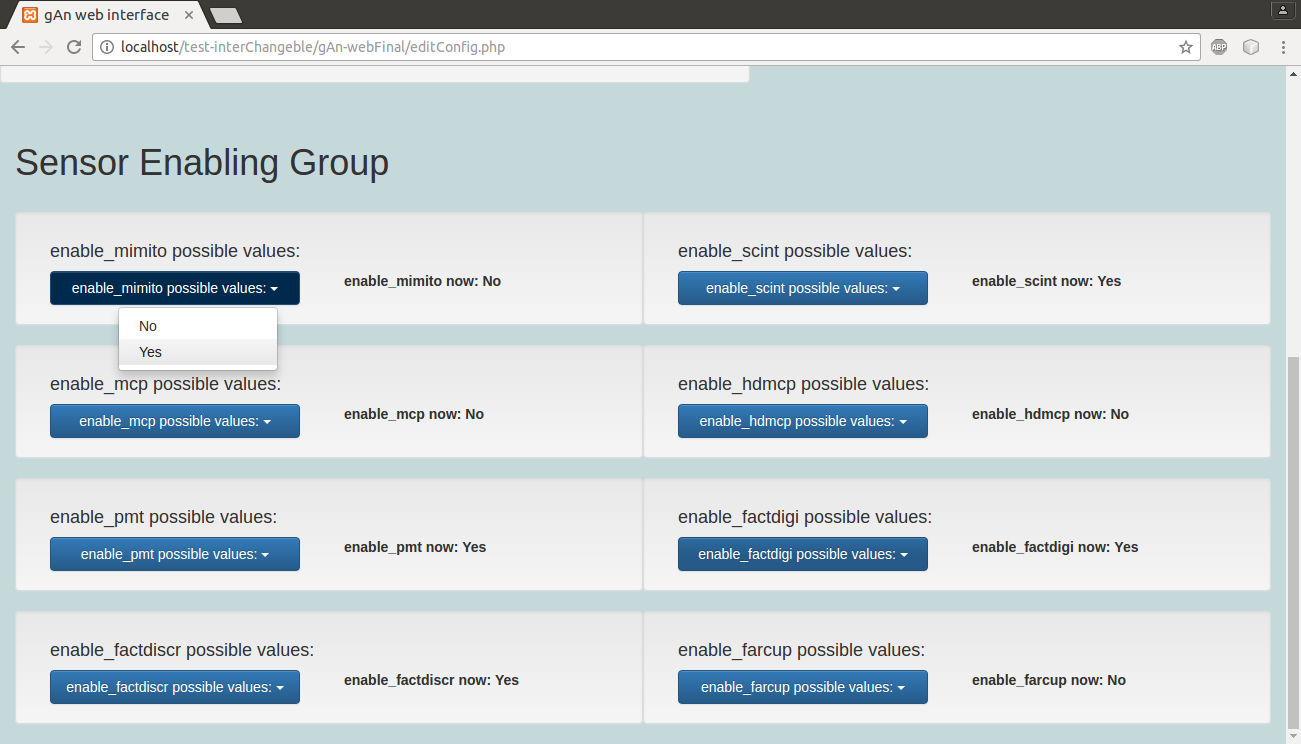
\includegraphics[scale=0.25]{ParticularYesNoConfig.png} 
\caption{ Final version: a group of dropdown menus }
\end{figure}  

\newpage

Output: 

There are some innovations. The first one is the navbar: now the user can find here all the most important commands. Before there was more buttons, distributed in the screen, and during the tests the users had problems to found them and to understand their functionalities. Now the navbar is more clear and organized:

\begin{figure}[H]
\centering
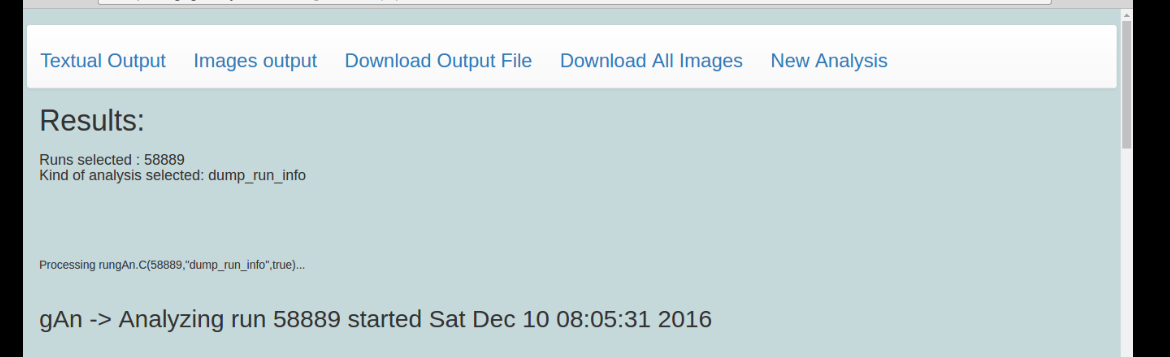
\includegraphics[scale=0.35]{LastNavbar.png} 
\caption{Final version: the Navbar}
\end{figure}  


Textual Output:

\begin{figure}[H]
\centering
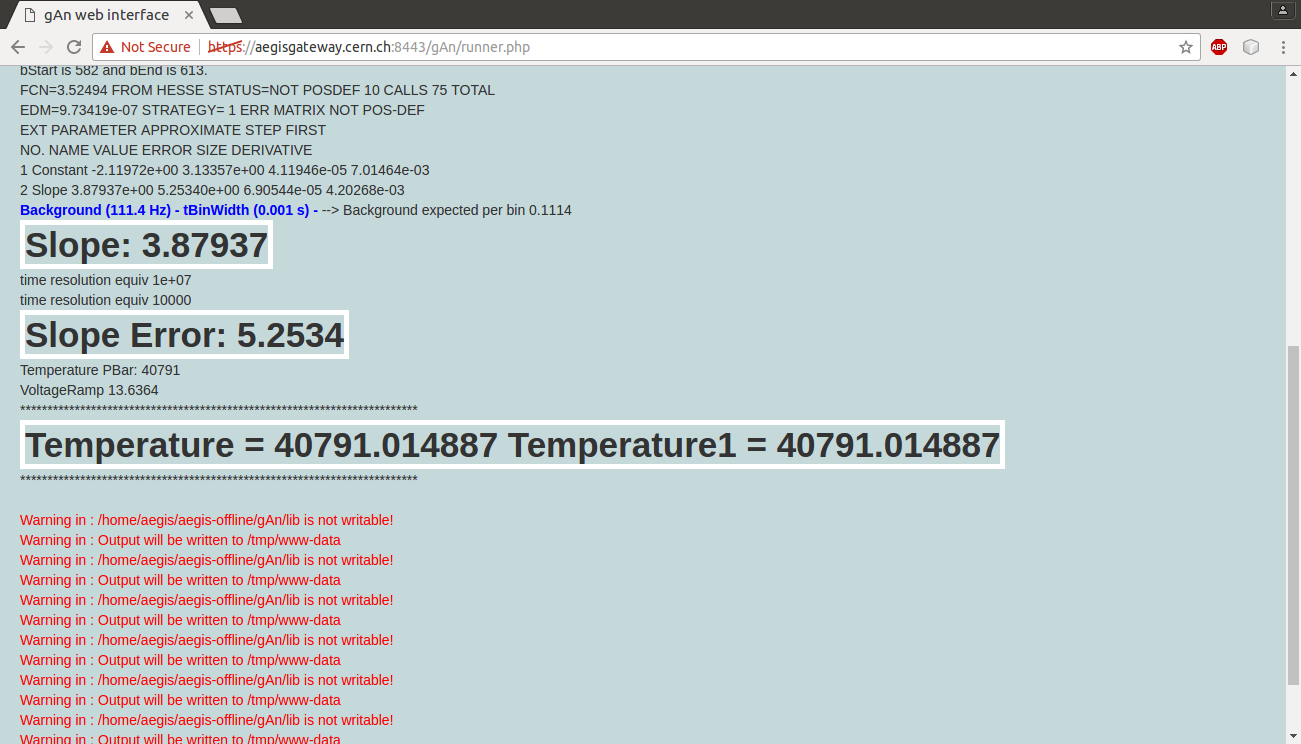
\includegraphics[scale=0.25]{LastTextualOutputHighLight.png} 
\caption{Final version: the output in textual version}
\end{figure}  

Here we can see out a textual output appears: there are more information, but in the 95 per cent of cases only a few are really useful, so they are highlighted with a special font and a big border (the hope is to use perceptive suggestions to advise the user about where to find what he searches). In this example we can see also some warnings: where something works wrong (or simply not perfectly) the system informs the user about the problem, with a red color, to ensure that he sees it. 

Let's make a confrontation between the same textual output before and after being formatted:

\begin{figure}[H]
\centering
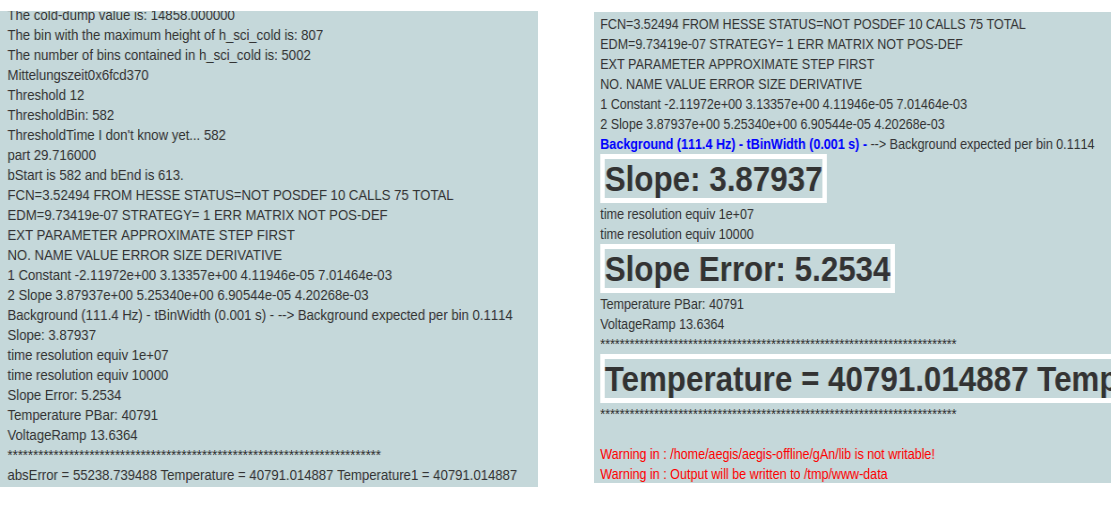
\includegraphics[scale=0.45]{TextConfrontation.png} 
\caption{Final version: formatted vs unformatted output}
\end{figure}  


Images output:

\begin{figure}[H]
\centering
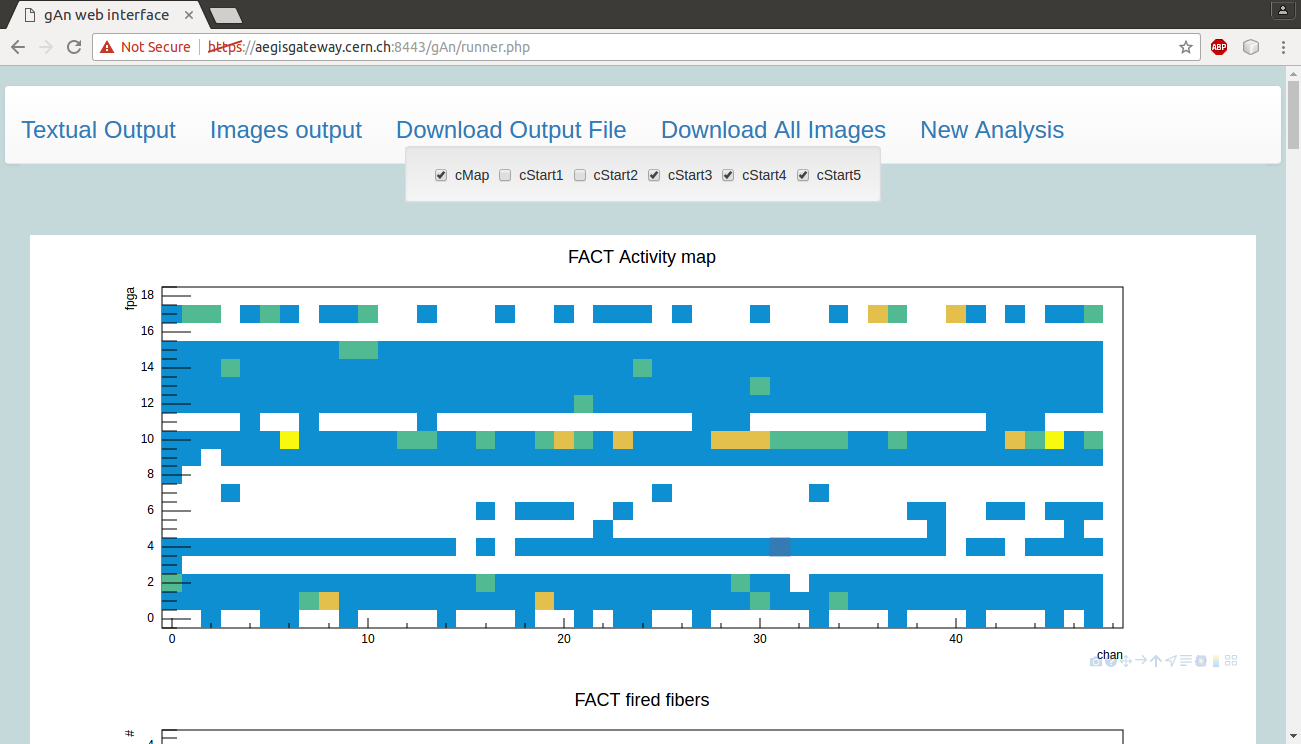
\includegraphics[scale=0.25]{ImageOutput.png} 
\caption{Final version: the output images}
\end{figure}  

Here we can see that there is no more the opportunity to select the dimension of the images (but still there is a zoom function in the image), or the layout, because none of the users never used these functionalities in the tests .. nor the possibility to choose a particular run of a group of images: this is because like discussed previous in this chapter the existing of the "kinds" of analysis makes this choice useless. Actually the navbar with these options is completely removed: the goal of this choice is to avoid the "information overload", so not to give the users too many commands and options, even more if these options are considered quite useless by the users.
Instead there is a list of check-boxes that if selected or deselected let the images appear and disappears. This feature is not determinant with 2 or 3 images, but sometimes the images are 7-8-9 so it is necessary.

\begin{figure}[H]
\centering
\includegraphics[scale=0.45]{ParticularHowToSelectImages.png} 
\caption{Final version: how the user can choose which images to show}
\end{figure}


An observation: sometimes the output is a list of images, vertically organized in a framework, some other times is a single image with more graph on a single sheets (a graph for each run inserted by the user as input, now all with the same color, but soon each run with a personal color); why?
The output is a single image on a single sheet when the goal is to compare different charts to see what is different, the output is an array of separate images when the goal is more related to the exploration, when the different images don't contain the same type of information. Sometimes is interesting make a confrontation between two images: in that case they are usually positioned horizontally. Who can decide what is the goal in each case? The solution is simple: who creates the analysis, so the back-end of this system codifies directly in the program how to show the charts in one or more sheets. This is because nobody better than who creates a particular analysis can understand what are the goals of this analysis.


\begin{figure}[H]
\centering
\includegraphics[scale=0.35]{ParticularConfrontationImages.png} 
\caption{Final version: Images that are meant to be compared}
\end{figure}   


Also in the "output image" case we observed that the users in most cases search in the images (almost) always the same information, so in some images the most important data (often they are dimension of peaks or integrals of spaces, or distances between peaks, or, in the case of charts with a time on the x-axis, auto-generated timelines about asynchronous events and triggers happened etc..) are directly written on the picture, like the following examples:

\begin{figure}[H]
\centering
\includegraphics[scale=0.25]{LastImagenotes.png} 
\caption{Final version: images with info}
\end{figure}   

\begin{figure}[H]
\centering
\includegraphics[scale=0.5]{ParticularFastReadInfos.png} 
\caption{Final version: other image with special info in a clear position }
\end{figure}   

There we can observe that the important information can be shown directly on the plot of the image (if they are graphical information, for example peaks, position of triggers etc) or in a special square on the top-right of the image (if they are not directly related to the image, but come from calculation or machine's settings).

\newpage

There is again the opportunity to access more information right clicking on the graph, of modifying it in various ways for example showing the graph in three dimensions: 

\begin{figure}[H]
\centering
\includegraphics[scale=0.25]{LastImageOptions.png} 
\caption{Final version: some options}
\end{figure}  

\begin{figure}[H]
\centering
\includegraphics[scale=0.25]{LastGraphImage2.png} 
\caption{Final version: other option}
\end{figure}  

Often the users in the tests had problems understanding that with a right click they could access these functionalities, so now there is a specific label on the right of the screen to inform them (this label is in fixed position, but became visible only if the user arrive with the scrollbar on the images):

\begin{figure}[H]
\centering
\includegraphics[scale=0.45]{LastImageLabel.png} 
\caption{Final version: label to inform the user about a feature}
\end{figure} 

There are some additional commands, that actually nobody used in the tests. Having on the screen commands that nobody uses is a potential source of confusion, but the developer is not absolutely sure about the idea of delete them. A good solution is to have them in the bottom of the frame of the image, not very highlighted, because they are not very important. Probably in a future confrontation with the super-users (is important to remember that this stage is never finished and always open to modification) these commands will be deleted.
They are in the following image:

\begin{figure}[H]
\centering
\includegraphics[scale=0.45]{ParticularUnusedControls.png} 
\caption{Final version: not frequently used controls}
\end{figure}    
% Chapter 8

\chapter{Users and Tests with them} % Main chapter title

\label{Chapter6} % For referencing the chapter elsewhere, use \ref{Chapter6} 

In this chapter first of all is exposed how the users are defined and what are their characteristics. Also, here are described the tests conducted with them and in which ways they are useful to improve the gAn Web's features.   

\section{User's Profile: why?}

Generically a correct understanding of the user is very important to adapt the features of an application to him; In this case is also more important, because the kind of users to that this application is intended to is quite particular.


\section{User's Profile: classification}

\subsection{Generic Characteristics}
In this part of the document we can try to classify the user:
The estimated number of users of the application is around at most a few tens.
All the users of gAn Web work as "Shifters" in the AEgIS experiment: so they work with data acquisition and (simple) data analysis.
A good advantage is that the users are already strictly defined, we have detailed information about them, and they are easily accessible for tests and co-developing.
Usually the typical user is quite young: around 30-35 years. This is because the most of the time personnel with a major seniority doesn't work with tasks related to data acquisition. 
Half of them are male, and half female: in this particular case we think that it is not relevant in their interaction with gAn Web.
A considerable amount of the users use eyeglasses, and probably some of them work too much time in front of a screen, but the kind of interaction designed with gAn is usually fast and isn't a big commitment for human eyes. We tried to avoid too many white backgrounds and the use of dazzling colors, but for the images' background they are considered acceptable to improve contrast and let the image to be more clear.  

\subsection{Education Background}
The cultural and educational level of the users is very high: almost all of them have a Phd, and they do a complex scientific job. They often have in mind a really structural model of the processes that go on in all the AEgIS experiment applications.

All of them have an extraordinary deep understanding of the particles physics: in particular they understand the technical terminology, the jargon in which the logbooks are written (because all the personnel, in shifts, write the logbooks) and the names of the sensors (this is quite important, each sensor has a proper name, they are very numerous, and the fact that the users can identify them easily is a big advantage). 

Other important information: almost every time a user uses gAn he is quite sure about what he is looking for. Situation in which the user searches a run number and reads generically the output of an analysis (or thinks about which is the correct analysis to use) is not common: in the most of the use cases the user is pretty sure about what is the information to search and what is the correct analysis. 

A different approach exists for the run number, in this case we must identify two different situations:

\begin{enumerate}

\item The most of the times (around 2/3) the user works with the last run, or the one immediately before. In this case is quite simple identify the correct run (the last is always shown on the application homepage).
\item Sometimes the user searches information regarding a past run, that he remembers to be interesting for some reason. In this case often the user remembers the date (the precise day, or the week) of the interesting run, but not the run number exactly. To manage this situation in the homepage there is a "view" of the RunLog, on that there are information about all the runs, organized by date and run numbers (the implementation of this view is a consequence of the tests with the users). 

\end{enumerate}

Most of the users are used to use the Linux's terminal, so they are used to quite complex but efficient interaction. A good advantage is that the users are very used to approach new applications, even complex ones, and they learn very rapidly: the advantage is that they are used to giving developers hints about what they expect from a new application, because they do it quite often. GAn Web offers them a way to interact efficiently like in the terminal but easier (hopefully). They also are used to have a feedback for every action they do (using the Linux's terminal you can always know if the program is running, if it is crashed, and what are its outputs).

One of the tested users is (also) a web developer, so his hints are particularly interesting because is quite expert in the creation of interfaces.
 
All the users have an excellent proficiency in English (they are used to speaking English in their work environment). 

\subsection{Models in the user's mind}
An interesting additional observation about the users is that more than half of them (mainly the most expert) have in mind a structural model about how do the processes work. In fact in their mansion there are tasks related to the design, the installations, the linking system of the sensors on which gAn is based. So more than half of the users use gAn Web understanding directly the processes that take place behind them. Adding to this, a part (in this case less than half, maybe one third) of the users have a good understanding of software programming so can also really understand "how" the application is working.

\subsection{User's psychological characteristics }
The style of reasoning is quite deductive: the users seem to act in a very scientific way: they observe the situation, they make hypothesis and they experiment them to check if they are true. From the test highlights that the users think mostly in an analytic way, using only seldom their intuition. In gAn Web we can observe that when they are for the first time in front of the application they observe the screen, reading all the tooltips, they understand (of better, they make hypothesis about) what each function does, and they test the functionalities making comments regarding if the application's behavior is the expected one. According the users' propensity the designer of gAn Web tries to let the application act like the user expects.   

Generically the users work in a quite enthusiast and positive way: the analysis done previous with the Linux terminal was quite time-consuming, so gAn Web is considered as an improvement (or at least, a step in the right direction) and the users seems to be quite happy to use it. All the people showed in the tests the maximum possible commitment and professionalism (in this way the opportunity to test the application directly with real users was very helpful).

It is possible to analyse the arousal of the users from the point of view of the Yerkes–Dodson's Law: the situation seems to be favorable: nobody of the user 
has problems with low arousal or too much performance anxiety (probably no one seemed himself under the judgment), so the personal activation of the users seems to be optimal.

\subsection{User's level of expertise }
At this stage all the users are beginners, but generically the application is simple and, except that the first moment for understanding the basic functionalities they can reach a good level of expertise. A big advantage is that almost all the users understand what the application does, which are the mathematical principles on which gAn is based, and how this application is integrated in their tasks.   
All the users are absolutely expert pc-users.
The two pilot-users play the role of super-users, able to be a bridge between the design of the application's interface and the needs of the users. They are also the developer of the pre-existent application, on which the interface is based. So they can be an extremely useful resource.  


\subsection{Environment}
The environment is a normal office. Often the users work in night shifts, and the only possible negative effect of the environment is the tiredness of the users, able to damage their arousal. 

\section{Relation developer-user and progressive sematization}
The developer of the application is a student in Software Engineering, and his domain is quite different from the users one. But in the time in which users and developer worked together the mutual adjustment between the two parts and the common approach to solve problems, united with the opportunity of use the pilot users (also supervisors) as bridges leads to a progressive semantization, so we can expect (hopefully) that under this point of view the developer has a deep understanding (or at least the deepest possible) of the real needs of the users.

\section{How the tests take place} 

This test is divided in three parts: 
\begin{enumerate}
\item
The first part is a direct observation of the user when he uses the application. It takes place during the shifts: both the users and the designer partecipated in this task divided in groups of 3-4-5 people, so this is a perfect opportunity, also because actually it is not a simulated test, is a real test on the field in a real work situation. This test is an observation of the behavior of the user with the application: the developer tells to the user only a little information: the fact that this application can transform a run number and a kind of analysis in an output. 
The first idea followed a pattern in which the developer asks to the user to use this application during the shift, in the situations that correspond to the expected scenario of gAn Web: in this situation the user talks about what he is doing, and makes comments, and the developer observes and takes notes about what happens (and this pattern was effectively applied with 4 users), but to test the biggest possible numbers of users and recover more information, in other cases the developer asks to the user to try to use the application in a simulated situation (not a really work situation) and to reason about what he is doing. The reason of this choice is that wait the moment in which the application can be used during the shifts to test isn't efficient (but still is a good resource) and "create" artificially the situation is a good idea to save time.

\item
The second consists in the proposition of a standard survey about the application to the user, to be compiled. This survey is the standard SUS survey. This choice is related to the fact that using a standard survey we can have an high quality already tested survey with precise and organized closed questions, able to give us an idea about the overall result of the interface. 

\item 
The third part consists in a brief discussion with the user (some chosen users, selected by their willingness to dedicate a moment to discuss about the application): the designer asks him in which way this application can be more useful and if there are in his opinion some good ideas to implement able to improve the helpfulness of the application. The discussion is quite free, but a fix topic is about what are the sources of the problems that the users had during the use of the application in the first part of the test. In fact the big limit of the observation of the users is that it is easy to find if there are problems but more difficult to understand why the problem there are and how they can be solved. So a direct confrontation of the user can overcome this limit. 
The developer tried to ask to the users some of the 9 questions proposed by Nielsen, but not in an automatic way, searching a more flexible approach and trying to follow the user and let him talk freely.
Another fix topic of the discussion is a generic request about tips and ideas that the users can have to improve the application (one of the interviewed user is also a web developer, who creates some applications and related interfaces used in the experiment, so in that case this second question occupied the biggest part of the interview, to exploit at maximum his experience in this field). 

\end{enumerate} 

\subsection{Preliminary observations}
It is interesting to observe that it is very important to encourage the users to criticise the application: if fact the developer and the users work together for some weeks, and it is possible that the users are too gentle in the judging of the application, because they don't want to be offensive. Instead, is necessary say them that all their critics are absolutely useful to improve the result, because the developer cannot understand alone what can be modified. 
 

\subsection{What the test is evaluating?}
Often some tests measure the time that the user needs to execute tasks to understand how difficult the interaction can be; but in this case the developer takes the decision of not to evaluate the time: all the processes in the AEgIS experiment are very time consuming, and this is not a problem, because the goal is not the efficiency but the effectiveness. It is not important if the user makes an analysis in a few seconds, it is important that he can use all the functionalities that he needs correctly to achieve his goal. So the test are evaluated in these dimensions: how many functionalities the users use? If they search a particular functionality the search from the beginning in the expected place? Do they find the correct command or they ask to the developer for a hint? Does the functionality that the user search exists? These are the interesting answer that we need from the tests.  

\subsection{Execution and Results}
The first part of the test, the one related to the observation of the users working with the application and talking about what they do, gave a big amount of useful information and lets the developer observe a good amount of problems and errors. 
The biggest part of the problems are founded by observing the behaviors of the user and asking directly to him if there is a problem: for example, if the user searches for a while how he can enable a sensor and has some difficult to understand how to do it, the developer can listen his comments, understanding his reasons about where he thinks this option can be, shows him where actually the sensor is, and understand that probably the location of the sensor option is not clear. 
Here is a list of problems found in this phase:

\begin{enumerate}

\item
Almost all the users tried very often to change a particular parameter by the configuration page, named "scint rebin", related to the thickness of the points that are fitted to create a function. Moving this parameter the user can modify a particular type of analysis named "TMeas", according to different exigences. Before the test was not so evident that this parameter was so important, and actually in the intermediate version it is not in the list of parameters that the web interface can modify. So in the tests the most of the user manually changed it by a text editor in the configuration file on the server: surely it is unacceptable and this problem must be solved to allow the application work in this particular situation.

\item 
The main options in the configuration page are related to the activation or de-activation of sensors, but the users actually don't use them very often, because  the default values are acceptably correct. So a good idea is to highlight other setting options, and move the rarely used ones in other part of the screen.

\item
In the page that shows the images the user can by a selector choose if he wants to see the images in a big, a middle, or a little format. During the test no one used this opportunity, and when the developer asked to the users if this control can be useful they simply say that the correct dimension of the image the "big" solution, with the image that cover (almost) all the screen in width. In this case the user can easily read all the information in the image. At this point is possible to observe that the "image dimension control" is useless, and it is a good idea remove it (or at least move it in another part of the screen). Also the other buttons in that group resulted not very useful, and also not very clear: this part of the interface must be carefully re-thought.   


\item
The interaction of the users with the personal output is particular: during the test the users read it rapidly, but actually they take from there only little information contained in 2-3 rows. Actually in each type of analysis in the most cases there are a few important information, and only in the other cases the user must read all the rest of the output (but in that cases he must). So a good idea is to highlight the more important parts (that varies based on the type of the analysis), to organize in groups the "sometimes important" parts, and to hide all the others (there are some rows that are reasonably important only in the debug phase, but before hide them it is better evaluate this point again with the super-users).

\item 
One of the worst problems is the maybe half of the users don't understand that if they right-click on the image they can access a lot of information such as other representation, drawing options, opportunity to zoom in or out, labels. In that cases almost all the users asked directly to the developer how to act this commands, because they are necessary to the correct use of the application. These controls are probably one of the biggest improvement between gAn and gAn Web, because give to the users new opportunities of understanding what is happening in the experiment through information related to the images (the previous version, before gAn Web, had only png-format images, without this controls), so the fact that the users often don't find it is a big deal. A solution can be create a label-advice to give the user a clearer vision.

\item
Some users, when is in the textual-output page, have some difficulties in finding the command to move to the images pages (and vice-versa): probably the button is not sufficiently evident in the screen. This problem can be an impediment with new users so it is important to solve it, re-thinking the distribution of the buttons in this page, that are actually not very clear. At the end the adopted solution is a complete re-distribution of the output pages, that now can be switched by a unique Navbar, that contain all the important commands.

\item
Users seems to be confused when they press start and must wait some seconds for the results, and some of them ask is the program is working correctly, even if there is an infinite progress bar and a "wait message". The wait time is longer that we expect, so it becomes a usability problem. This is unacceptable, but we think that the waiting time is related to the server that is too busy: in fact this is not the only application that works on it. In the spring 2017 we are going to format the server and re-distribute some applications, so we hope that some seconds of waiting will become less than one second (so, acceptable). According to this fact we hope to solve this problem working on the machine, not on the interface, obviously if on the new-configure server the problem will persist we'll have to create an exit-strategy for the user to eventually stop the waiting, and give him more precise temporal information about the remaining waiting time, maybe with a percentage progress bar instead of an infinite one.

\item 
It would be a good idea think a system able to help the users to link the run numbers to something they search without using human memory: a view on the RunLog is necessary.

\end{enumerate}

The second part, the one related with the surveys, has as goal to give an overall idea about the utility of gAn Web. This part of the test was unfortunately a bit less useful, because the results seemed to be too high if compared with the amount of problems founded in the first test (probably the users simply tried to be gentle with the developer). Generically the strategy based on the survey was used no more after this attempts (the direct tests with the users seems to be more promising).

The third part, the one that consists in the discussion with the user, was very helpful: almost all the selected users proposed new ideas (all of them are useful, the most of them are effectively implementable), and new functionalities. Some functionalities was asked by almost all the users, so they probably are absolutely important to improve the interaction quality. 
The biggest part of the users observations and ideas is coherent with the observation made observing them 

Here is a list of observations obtained in the third phase, through discussions with the users:

\begin{enumerate}

\item 
Probably inserting a tooltip on each button the overall clearness of the product can grow, but it is important to be careful with the risk of covering with the tooltips other buttons. For some commands the tooltips must be more long and precise, because they are not so easy to understand (the pilot users can understand them better because they are very expert in the domain, but it is not always clear for everybody; a more clear choice of what to write in the tooltips can make the application more usable).  

\item
Actually the names of some buttons are not clear. At this stage the developer is not a deep expert of the domain, but probably is more expert than at the beginning, so a general re-discussion of all the names of the buttons (and related tooltips) seems to be a good idea.

\item 
The application is though to be used in the standard AEgIS' experiment screens, that are quite large. But sometimes the users use it from home, and the application must be adaptive to smaller screens (there are some little problems, such as buttons overlapping).

\end{enumerate}

\subsection{Is the testing finished here?}

No it is not. The application is entering right in this moment in the standard working processes of the AEgIS experiment. The web application can be prepared to meet the exigences that exist right now, but according to the dynamism of the experimental environment is highly probable that the continuous changing of the back-end (gAn) will lead to a need of constant upgrade of the requirements. In this situation the users will continue to utilise the application, to find new problems, and this fact will route the developer to a continuous process of adaptation.     
% Chapter 8

\chapter{Patterns} % Main chapter title

\label{Chapter8} % For referencing the chapter elsewhere, use \ref{Chapter7} 

Developing gAn Web it was decided to design together the physical part and the conceptual part. This is the holistic approach to design. In this project the users play a special role: they are absolutely participatory, they are an important part of the developing team.
The point is that in this project the needs of the users are very particular, and very hard to understand for a person who doesn't work in the physics world. So the users must take part in each decision and give continuously opinions and feedbacks, to avoid misunderstandings and to obtain a good result.

\section{Used patterns}

The use of some patterns can help the designers to create a better application reusing good solutions already known.
The main source of patterns of this project is the website \\ \url{http://designinginterfaces.com/patterns/}, based on the book "Designing interfaces", written by Jennifer Tidwell, in the edition of 2010.

\subsection{Clear entry point} 

In each page there are only one or two entry points, clearly visible for the user.
The first entry point is always the arrive from the logically previous page, and the second is in case the result of a "go back" button somewhere.

This result is quite easy to achieve because in the application there aren't an incredible amount of pages, and in each page, according the logic, is quite easy to understand where the user desires to go. 

To enforce this result there is a block system: if the user accesses inserting directly the URL in the browser for example in the configuration page without passing through the normal path of the program the system understands that some cookies doesn't exist and re-forces automatically the URL to the first page: the Login one. This is a designer's decision according to that the limitation of the freedom of the user is acceptable to ensure to show him always consistent pages with consistent contents

In conclusion in each kind of task that the common user executes with gAn there is a "standard" path, hopefully very easy to find. 

\subsection{Wizard}
The fact that each task in gAn has a "standard" path leads that each task executed with the web interface can be carried out using a wizard. The user loses some "freedom of movement" in the application, but in this way he is forced to follow the right way and can avoid easily errors or omissions.
Is this a limitation? We must observe that if, for hypothesis an user is interested only in a textual output the program forces him to see also the image-based output, but, both output are in the same page, and the navbar allows the user to go rapidly where he wants.

\subsection{Spatial memory}
In each page the opportunities to move to another page (back to home, new analysis etc) or to execute tasks (confirm, download something, show images) are concentrated in the navbar on the top of the screen. The hope is that in this way the user can automatically associate the position of the navbar with the concept of "commands". All the navbars in the program have the same buttons? Not exactly, but all the important commands are in a navbar. The goal is to create a "link" in the mental model of the user: this link is between "I search an important command" with "navbar position".

\subsection{Grid of equals}
This pattern recommends to position the elements in the screen in a way that creates a "grid". All the elements of the grids must have the same visual weight, to seem equally important to the user's eyes (unless hide some of them is the goal of the developer, there is a discussion about this regarding some commands in the image output page).
This pattern is used in the page that allows the user to edit the configuration file of gAn, this disposition of elements is useful to give the user an ordered exposition of the editable options in the file.


\subsection{Responsive enabling}
There are some buttons in the web interface that executes tasks which need some pre-conditions. For example: to start the gAn program it is mandatory to insert one or more runs as input for the program. If this condition is not achieved the button is inactive, and only when the user inserts correctly the requested values it became clickable. A similar behavior happens in the configuration page. In this way is possible to avoid useless errors and wastes of time, without create frustrating experiences for experienced users. In the intermediate version in order to say to the user if the button is clickable or not we used the colors red-green, but in the final version the use of the standard Bootstrap's graphic that for this point prefers to use the variation of opacity, seems to be a better idea (for aesthetic reasons).   

\subsection{Progress indicator}
The starting of gAn is a complex task that takes some seconds. This waiting can be disturbing for the user, who can think that the program is crashed. Another problem is that is quite difficult at this moment estimate the waiting time with precision. A solution can be create an infinite progress bar, that cannot show to the user exactly how much time he must still wait, but can inform him that the system is effectively working and has receipt his request. In the finished product, with a completely working server, we expect that the waiting time is something around 2 seconds (in the worst case) , no more. 

\subsection{Go Back to a Safe Place}
In each screen the user can easily return to the homepage , that is the common start point of all the possible tasks. When the user returns at this situation the program re-starts asking him if he prefers a multi-runs analysis or a single-run one, so the program is ready to start a new task. 

\subsection{Liquid layout}

This useful pattern recommends to create a dynamic structure able to adapt itself automatically to the screen's dimensions. The concept of "adapt itself" doesn't include only the ability to modify the dimensions of each object, but also to modify the layout of the screen. This pattern is very useful in applications that must work both on laptops and on mobile devices. In the particular case of gAn Web the users never use mobile devices (a correct analysis request a big screen), so the application has to adapt itself only to screens with a dimension of minimum around 10 inches. For this reason the automatics system of object-dimensioning provided by Bootstrap (based on the partitioning of the screen in columns and sub-columns) is sufficient to ensure that all the system is usable by all the "target" screens. In fact all the objects that compose the system's graphic can adapt themselves easily to all the expected screen dimensions. 


\subsection{Hover tools}

This kind of helper allows the user to get information about the tasks that each object can carry on just moving the mouse over it. 
The interface of gAn Web is quite simple, but for a new user is useful to have a some tips about the components potentialities. Bootstrap provides some easy commands to create the tooltips accessible by a "on hover" event, giving to the developer a fast way to implement this pattern. What to write in these tooltips is not trivial, the developer needed the advice of the super users (sometime also of common users) to be sure about what to write. 


\subsection{Harmless default}

This pattern is used in 2 ways:
\begin{enumerate}

\item In the homepage, where the user has to insert the run numbers (before he can press the start button) some place-holders are visible. 
These place-holders aim to teach the user how to insert correctly the numbers.

\item Another use of this pattern is related to the page that aims to modify the configuration file of gAn: here the user can see set the last known working values, avoiding to re-insert values that he doesn't want to change. He also can, through the related  button, re-set all the configurations to default values.

\end{enumerate}

\subsection{Same-page error messages}

This pattern allows the user to understand immediately if and where there is an error in the inserted values, showing him a visible message in the page able to explain him how to correct the error. In most cases in gAn Web the values are inserted using dropdown menus, so it is impossible make errors (or better, it is impossible choose inconsistent values..), but in each part where there is a "free" input field this pattern is used: if the inserted value doesn't meet the requirements of a validator a message appears on the screen explaining to the user what to do to solve the problem.

\subsection{Alternative views}
This is an example of pattern that we tried to use, mainly in the intermediate version, but at the end we decided to leave. 
This pattern proposes to let the user choose among alternative views that are substantially different from the default view. 
GAn Web tried to apply this pattern in the intermediate version where the system showed images to the user: the user was enabled to choose if see a static image in png format, that is simple and contains all and only the needed information (or better, the information that the designer thought the user needs), or a dynamic, modifiable and navigable image in Root format, in which the user can decide exactly what to see. Also the user was able to choose the dimension of the image (little, medium, big). But to the test with users we found that actually almost nobody used this opportunity: the users always chose big images, root like version. So this choice opportunity was removed. But a smaller example of this pattern is still used: when the user see and image that contains more than 2 dimensions he can see it both through a projection on the plate and through a 3-D rotatable and accessible image.


   
% Chapter 9

\chapter{Web Development} % Main chapter title

\label{Chapter 9} % For referencing the chapter elsewhere, use \ref{Chapter1} 

%----------------------------------------------------------------------------------------

This chapter aims to explain what choices were made and why from the web development point of view. It is interesting to analyse which are the particular requirements of this software and what solutions were chosen to satisfy them. 

\section{Requirements from the Web Development Point of View}

From the Web Development's point of view the first step to do is to identify what are the most important goals to achieve. They are uncorrelated but not conflict with the requirements already analyzed related with the Human Machine Interaction's point of view. Following there are some observations:

\begin{enumerate}

% 1
\item
The first thing that it is important to guarantee is a strong division between front end and back end. This is because both part are important, but the way in which they work are very independent, and they can evolve in different ways.
As explained in the previous chapters the front-end, so the way in which the information is presented to the user is a particularly sensitive issue that needed a special attention and a deep analysis related to the interaction; The back-end is also important because needs to work on particular topics related to the communication with ROOT Framework, the security, the persistence of data. An important observation is that the front-end changes in the time, according to the new features and in reaction of the observations of the users, but the back-end changes faster. The challenge of the front-end is the needs to remain more stable and be re-usable when the logic behind, the back-end changes. For example: almost twice a month the algorithms of the existing analysis of gAn change, and also new analysis are added (sometimes some old ones are removed). The output of the back-end changes rapidly, but almost always the front-end, that is flexible can manage automatically the situation showing the results to the users in an organized way. Also the drivers able to trigger the changes are different: the users for the front-end, the scientific progress of the experiments for the back-end. If these parts are completely (almost completely) independent it is surely all more simple. In principles it is also possible a complete substitution of the back-end: both with a different program able to implement analysis of data of the AEgIS experiment or with a completely different program able to work with runs, to give outputs formatted in text and images, and to be configured by an xml file.

%2
\item
Another quite important point to keep in mind is that this application will be maintained and probably modified by people that aren't specialized web developers. So it is important to maintain the code as simple as possible and to "hide" the complexity where a complex structure is unavoidable. For example, the functions able to read and write on files, to extract histogram from vectors, to apply "regular expression" to verify the format of a file can be packed into functions able to be simply called without expect expertise from the programmer. All the decisions related to the paradigm and the environment to use for this project may take consideration about the fact that simplicity is a fundamental requirement.   

%3
\item
The logical separation between client and server implies that a way to communicate is needed. A simple communication based on Post and Get is quite effective, but a more structured communication based on exchange of complex object seems to be more re-usable, and simpler to maintain and modify. From this point of view Json language gives a standard well-known solution, simple, efficient, and effective to solve this issue, but also other technologies were analysed: in particular we are looking for technologies able to send human-readable messages (this is useful in debug phase). The best alternative to Json is probably Yaml, that seems to be more readable, but also a more immature technology. 

As we can see Yaml is very near to the way in which a human thinks, and has the advantage to be a superset of Json (so each Json message is also a Yaml message, but not viceversa) but this technology is less diffused and probably for the next programmers who will work on this application or will need to communicate through HTTP it can be a problem be forced to work with a not-mainstream technology, and difficulties are able to overcome advantages. 

%4
\item
The program of data analysis (gAn) needs to be configured. Some of these configurations are accessible by the user, some aren't, but in both cases it is important to give a structured way to persist the configuration of the application. The first idea is to use a simple text file to achieve this goal, but with the growth of the file a more formal solution becomes preferable. Xml is a good solution, because it is a diffused standard and there are a lot of API and libraries able to help to write and read it easily.

%5
\item
A simple but precise way to evaluate the formatting of a string or a group of strings is needed to ensure in every moment that the program is working with the correct value. For example, it is important to ensure that if the user is inserting a run number the entered value is effectively a decimal number: in other case the front-end can advise the user of the error. This first example is related to an inadvertent error, but it is important to consider also other situations when, for security reason, immediately before save a number in a file, or immediately before insert a number as a variable in a bash script the application needs to ensure that the value is compatible (so, has the same format of the expected one). There are some solution considered in order to avoid problems and formatting objects correctly, the two effectively used are regular expressions to certify if a string respect some limits, and some standardized functions provided by Php to check if in a string there are dangerous commands.
 
%6
All the software must work easily with the Root Framework, so communicate with it using APIs or other ways to interact with gAn. This is not always simply, because Root provides some APIs to communicate with languages used in web developing but there is a big lack of documentation. Often, in absence of documentation for some needed functionalities the best way to work was check directly the open source code of the APIs to understand the functionalities gave by them.

\end{enumerate}

\section{Why a web solution?}

Before start to work with this project using web development some other solution was evaluated:

\begin{enumerate}

% 1
\item 
The first solution considered was simply work with the commands of a common linux terminal. This is the solution implemented for gAn. This solution is surely powerful and effective, because gives the maximum control on the possible commands, allows pipelines, gives an immediate feedback in every moment (these features of the linux terminal are often ignored). However this is not the best possible available solution, because it presupposes a perfect understanding of the behavior of the program, and a very good memory to remember all the commands and all the possible analyzes. 
This solution is no longer used for the final application itself, but it is still very useful to debug the application in case of errors.   

% 2
\item
Another analyzed solution was the creation of a standalone application, with an advanced graphical interface, able to perform analyses on a common laptop or on the computers of the AEgIS control room. This solution is able to use all the advantages of the application of the human machine interaction science, but it is quite limited: in a hypothetical situation with this solution applied it would be very difficult give to all the users the same version of the application (that is changing continuously). So in that case a system able to check automatically the application for updates every "x" days would be necessary, and the total amount of complexity would be quite high. Other problems with this solution are that it would be able to work only with the LAN of the AEgIS Control Room to access the data that are stored on dedicated hard disks, and the computational power of a common laptop would have some problem to analyze data in a reasonable time (the data at the moment are some terabytes, but in the future this amount will probably growth rapidly).

%3
\item
Probably the better possible solution (the adopted one) is the web application. So with simply a web browser also a low quality laptop can access information, and both the data and the application are always at the last version (the application change quite rapidly, but actually new data are added every some hundreds of seconds every days when the machine is working.. so only a centralized application can meet the need to react to the continuous modification of the situation).
In this way the user doesn't need to install nothing, and this is an advantage because the practice shows that the installation process of gAn is not so linear and shows often configuration problems (the behavior of gAn is linked to the version of Root Framework installed on the machine, the different versions are not perfectly compatible). Another advantage of this solution is that in this way only the server needs to manage the problem to recover the data (at their most recent version) and to store them in an intelligent way. Furthermore the computational power of the server is probably more suitable to execute the requested analysis. It is important to reason about the possible request of parallel execution from more users at the same time, but considering the number of the total user of this application, that is around at maximum a few tens, the charge on the server to satisfy the multiple requests is not so high.    

\end{enumerate}

\section{Different hypothesis about how to implement the project}

After being sure about the choice of implementing a web solution it is important, considered the requirements take some decisions about the way in which work.
For the client side the situation seems to be clear: a HTML5 and Javascript solution, together with some kind of CSS processing technology, can meet all that is needed.

For the server side the challenge is a bit more open: there are to important decision to take: which programming language is more suitable for the exigences and which paradigm to adopt. This two question are in this case very linked together, and there are three solutions each one with pros and cons:

\begin{enumerate}

% 1: procedural PHP
\item
The first solution is simple: using Php with a Procedural approach. Php is born to be a procedural language able to work in the server side, and this approach can guarantee the simplest way to meet our goal. In particular this solution will allow also people that are not specialized in web developing to work easily on this project. On the other hand this solution is not very structured, and in a big project, specially with a numerous group of people that needs to work together will become full of problems.

% 2: OO PHP
\item
An alternative solution is again Php, but adopting the Object Oriented paradigm. This solution is probably more suitable for big server sides, more easy to maintain and to extend. But Php is not born as OO language, it supports the concept of object only from the 5th version, and a native OO language can be a better solution. This fact take us to the third choice:

% 3: OO JAVA
\item
Java is a natively Object Oriented language, and Jave Enterprise Edition is perfect to work on an application server like apache. This is a very structured solution, and we can use also very good frameworks like Spring to create a very well organized server side, scalable also for big projects. But there are also bad sides: this kind of application is more complex, needs specialized programmers to be modified and is not very good for little server sides. 

According to our exigences, this server side is not so big, the application is quite similar to a procedure, and mostly of the developer in the AEgIS experiment come from experiences with C, so are used to work with the procedural approach. At this point the decision is to work with Php, adopting a procedural approach.  

\end{enumerate}
 
\section{The simple solution: MVC pattern}

The application of the Model View Controller pattern is usually a good idea in Web Development, specially in an application that needs to be rapidly modified and needs a special attention to the maintenance. This pattern is perfect when it works with an object oriented project, but we can implement its logic also with a procedural approach.

We can start with a precise definition of what a MVC pattern is; according to Wikipedia:

\begin{quote} 

Model–view–controller (MVC) is a software design pattern for implementing user interfaces on computers. It divides a given application into three interconnected parts in order to separate internal representations of information from the ways that information is presented to and accepted from the user. The MVC design pattern decouples these major components allowing for efficient code reuse and parallel development.

\end{quote}

The following figure can make the point more clear:

\begin{figure}[H]
\centering
\includegraphics[scale=0.25]{MVC.png}  
\caption{The general structure of the MVC pattern}
\end{figure}    

So the goal is to divide the application in "independent" modules:

\begin{enumerate}

%1, VIEW
\item The view is the surface of the system. In this project it is created with Html, Css, Javascript (with some parts of Php, used to create through the "echo" command part of Html code that are repetitive, for example lists ). The design of the view in this kind of projects is particularly important because the application needs to represent particular kinds of information to particular kinds of users, and both the importance and the special feature needed by this interface are explained in the previous chapters. In the MVC pattern the view is the part less able to "reason" its goal is mainly related to the representation of information. In this project some kinds of representations are quite complex, but this complexity is managed by other tiers, and the view needs only to show the users images, html constructions, and artefacts to access graphics. So the view is the client side? No, it isn't: in the client side there is also a part of the controller, able to interpret the inputs of the user and send them to the logic of the application.

%2, MODEL
\item In the MVC the model is the central module of the pattern. It contains the application's behavior and must be independent of the user interface. Its primary goal is managing the data of the application. In gAn Web it is a complex situation: excluding some little data related to the configuration and other minor form of persistence, the main data related to this application are the outputs of another application (gAn). If we consider the whole system the model of the composed application is represented by the raw root files taken in input by the system. Their loading, interpretation, analysis and activities related to the update of the view are the main activities of the model tier.   

%3, CONTROLLER
\item The main goal of a controller are related to receiving the command of the users, the interpretation of these commands, and the consequent actions to change the state of the model. In gAn Web the controller is represented by the javascript functions able to check, interpret, and send to the server the desires of the users, and the Php scripts able to receive this commands, start the cycle of analysis of the program, and work directly with the model 


\end{enumerate}

In this explanation of the theory the MVC seems to be perfect, but in the application some further consideration are needed.

\section{The alternative solution: MVVM pattern}

In this situation it is perfectly clear what is the view and what it needs to do, and also it is quite clear what functions are surely related to the model. The definition of controller seems to be more nuanced: it is clear that this tier needs to receive the input of the user (and to manage it, that in some cases is not so simple), give them to the model that implements the business logic of the application and send to the view the results, so its role of "glue" is clear, but during the practical implementation an observation has grown: actually some functionalities that in the theory belongs to the controller, such as managing the complex interaction of the users when it works with the "alive" images provided by root and give him back a real-time feedback on the screen are in practice considerable part of the "logic" of the presentation, and furthermore their logic is implemented in the same methods able to read informations from the data so in some cases the strong division between view and controller seems to be less strong. 
In practice in this case a "fat view" manage the data-binding talking with an extension of the model, because this is the smartest way. 
At this point it is important to consider if in this project another way can be followed: applying a variation of the MVC: the Model View ViewModel pattern. 
In this pattern instead of the controller there is a component named ViewModel that allows the view to implement a logic, for example in this case interpreting the desires of the users and calling directly model's methods, and giving back to the view an image, modified in real time, in svg format. 

This pattern is less mainstream, but in this case can provide a more direct way to manage complex user interactions, at least in the page related to the output of the program, where the interaction user-data though images is quite complex. 
However it seems to be not perfectly suitable for all this project, and an intermediate solution can be adopted it only in little parts, where it can really be useful, in derogation of the MVC, that is the main pattern of this project.


 
\section{Other Used Technologies}

The adopted technologies for this project are generically the standard ones of a web application project, but some of them deserve some little explanation:

\begin{enumerate}

%1 sass
\item
SASS:
\\
\noindent
Syntactically Awesome Style Sheets is a language that aims to simplify the tasks related to the CSS files. The goals of this solution are not related directly with the functionalities of the application but more with the aesthetic of it.
The normal CSS language is simple and well organized, but using Sass we can further improve its features:

according to its official documentation :
\begin{quote}
Sass is an extension of CSS that adds power and elegance to the basic language. It allows you to use variables, nested rules, mixins, inline imports, and more, all with a fully CSS-compatible syntax. Sass helps keep large style sheets well-organized, and get small style sheets up and running quickly, particularly with the help of the Compass style library.

\end{quote}

In other words we can use Scss to create files similar to the normal CSS files, but with some improvements, such as nesting based inheritance and compile automatically them in normal CSS files, that are understandable by all the modern browser.

Some interesting features of Scss that can help this project are mainly two:
first of all the fact that Scss admits the concept of variable, so is more similar to a programming language that CSS. Second, probably more interesting, the existence of the nesting inheritance, in which the classes that are included in other classes full inherits the parent's features. This structure allows to produce elegant, better organizer, more reusable CSS code.

\item
Bootstrap:
\\
\noindent
This framework is mainly aimed to create a responsive (partially adaptive), well organized front-end. It is not a complete framework, so it doesn't involve all the logical part of the application, but only the front-end of the web part. This fact is important because ensures us not to create conflicts with the Root Framework on the back-end, and if in a future the back-end part of the application will be strongly changed (it is quite likely), the existing strong separation will avoid without problem conflicts with this technology. Bootstrap is a not-invasive, light structure, that carries many advantages, but for this project there are in particular two Bootstrap's features that invite us to work with it: the availability of a responsive structure created with very simple commands and the existence of a lot of pre-produced standard graphic artifacts. 

The first one is quite useful for any web project, because Bootstrap allows to divide the screen in twelve columns and assign to each component a number of columns to occupy (recursively, each component can in turn be divided in twelve columns and so on). This functionality can link easily the dimension of the component to a screen size and redistribute the components in the screen automatically if the dimension of the screen changes. There are also more advanced structures that allow to easily tell the component to occupy a different number of columns or adopt different behaviors if the dimensions of the screen are particularly little, giving to Bootstrap an interesting role in the development of web applications for the mobile world, but in this case the application is thought to work on a laptop or on a pc, so the general behavior is sufficient to satisfy the requests.


% %TODO %TODO %TODO %TODO %TODO %TODO  caccia una foto di bootstrap con le colonne qui

The second is the availability of a big amount of already implemented graphic objects such as buttons, fields, widgets. This allows us not only to save time (implementation of the style sheet of a widget is easy.. the time saving would be actually little..) but mostly to re-use solution that was created by specialized personnel with graphic design experience, so thought to have the strongest possible affordance. Another interesting point is that Bootstrap is quite diffused on the web, many sites are created using Bootstrap's artifacts, so the user can re-use his experience to understand the meaning of some commands. 
  
\item
Json:
\\
\noindent
Json is a smart way to communicate between client and server.
It is an open format that uses human-readable text to transmit data objects consisting of attribute–value pairs. The interesting point of this technologies is that it is (quite) easy to read by a human. This feature is very useful in debugging phase.  
It is the most common data format used for asynchronous browser/server communication, largely replacing XML, and is used by AJAX. In this application each server module produces in output Json-formatted information, and the clients can (using javascript) interpret these information and use them to build the page, and communicate actively with the server sending him requests formatted using this standard.
The diffusion and language agnosticism of Json allows it to be a common languages among different applications, and makes the parts of gAn Web more independent: if we want for example to replace only the client side we can simply build a new client side able to communicate with Json without touching the server. 

\end{enumerate}  

%TODO %TODO %TODO %TODO %TODO %TODO  INSERT AN IMAGE WITH JSON TO EXPLAIN WHAT IS

\section{General Schema of the project}

In the following picture we try to explain the general structure of the project; This picture isn't a standard UML graph, because a more free and informal graph can in this case explain in a probably less precise but more simple way what are the roles of each part. In particular, in this picture there are both software and hardware components, because we want to clarify what is the generic flow of the system (not the flow of the software system, but the global flow of information in the AEgIS experiment). To meet the goal of explaining what are the main actor in this situation some particulars are omitted, which the aim of exposing only what we want to clarify.

\begin{figure}[H]
\centering
\includegraphics[scale=0.25]{generalAEgISImage.png} 
\caption{The generic structure of the experiment}
\end{figure}
   
Through this image the general situation is more understandable: gAn Web is the whole client of the application, and occupy also a part of the server. The view is the front end of the client, the controller is the bridge between the view and the model. We observe that the controller is divided in two part: the one on the client and the one on the server, and these parts are strongly separated and able to communicate with json (actually, this explanation of the situation of the controller is simplified, as exposed in the previous paragraphs related to MVC and MVVM). It is very easy if needed to exchange the client or the server with another, and this leads that whereas the concepts of view and model are clearly defined and quite simply the controller is quite smoked (de facto, in the implementation of the images page the adopted solution is a MVVM). DAQ is the system of hardware and software able to take information from the machine and put them into raw, unfiltered Root files. DAQ is a very complex and heterogeneous machine, its description is not part of the goal of this document, but its role of information transporter is a key-role of the whole system. Also the AEgIS' experiment machine is a complex system, partially described in the first chapter, its role is to be the physical source of the whole information, the beginning of the system.

        
% Chapter 10

\chapter{Conclusions} % Main chapter title

\label{Chapter 10} % For referencing the chapter elsewhere, use \ref{Chapter1} 

%----------------------------------------------------------------------------------------

In this chapter some important points of this document are summarized, and some observations about the future of this application are expressed.

\section{Conclusions}
The first thing that we can observe is that the result of this project is a fusion between the studies of the needs and characteristics of the users and the ways in which this software can meet their needs, and an organized development of the product using web technologies. The most important needs emerged in this application are the flexibility, so the ability to be adapted continuously to a changing environment and the ability to understand the features needed by a particular class of users.


In this cyclical process of development, after much trying and re-trying, we can surely say that we have tested a lot of different ways to give the user the best possible product. The big modifications between different stages, both the ones derived from the pilot users, and the ones derived from the general users probably identified the most of the problems on this application, that now, with the final version are hopefully solved. At this point we can recognize in the adoption of a cyclical process of development the best choice made in this project, the most able to produce added-value to the result.

A good advantages that we have enjoyed during the development is surely related to the possibility to get hints from the pilot users, that are both users and supervisors, and surely gave a big help to correctly interpret the needs of the typical users. Also the availability of the general users to test the application and to help with ideas and opinions was surely important.

I conclusion we must observe that the needs of the users are not stable, are continuously changing, and the rapid evolution of the web technologies makes very unlikely to consider this application stable in the time. So, even if gAn Web is designed to be easy to modify, and in case to be enriched with new functionalities, the biggest challenge for the future is try to maintain the application up to date in a unstable and dynamic environment.  

  
\end{document}  
